% $Author: oscar $
% $Date: 2007-09-23 11:56:47 +0200 (Sun, 23 Sep 2007) $
% $Revision: 12130 $
%=================================================================
% Luc Fabresse (LF)
%% relecture (et reponse): Martial Boniou (remarque: j'ai mis les morphs au masculin apres mure reflexion.
% respecter la typographie française ? si oui, alors il faut revoir tous les itemize car il ne doit pas y avoir de majuscule après un ":"
%% reponse: normalement il ne doit pas y avoir de majuscules
% "System browser" laissé tel quel comme dans les autres chapitres déjà traduits
%% reponse: parfait
%  traduction de "class side"  j'ai mis "côté classe"
%% reponse: c'est ce que j'ai mis aussi
% problème de sens dans le SBE anglais: caption fig 12.3 : "The metaclasses of Translucent its superclasses"
%   traduit par : "Les méta-classes de TranslucentColor ET ses super-classes"
% relecture : Rene Mages 21-12-2007
% update: Tue Dec 25 22:32:45 CET 2007
% martial: convertir ``mon texte'' en «~mon texte~» pour franciser +
% j'ai mis des \ct{} au lieu de \lct{}
% relecture : Rene Mages 10-01-2008
% adaptation pour PBE - martial - Thu Sep 10 19:46:40 CEST 2009 
% relecture : Rene Mages 12-01-2010
% relecture : Rene Mages 12-08-2010
% relecture : Rene Mages 17-04-2011
% $Author: oscar $ $Date: 2009-08-17 12:10:55 +0200 (Mon, 17 Aug 2009) $ $Revision: 28502 $

\ifx\wholebook\relax\else
% --------------------------------------------
% Lulu:
	\documentclass[a4paper,10pt,twoside]{book}
	\usepackage[
		papersize={6.13in,9.21in},
		hmargin={.75in,.75in},
		vmargin={.75in,1in},
		ignoreheadfoot
	]{geometry}
	% $Author$ Martial
% $Date$ Wed Oct 10 13:34:55 CEST 2007
% $Revision$ source: SBE 12715 
% Last Changed Date: 2007-10-08 21:32:45 +0200 (Mon, 08 Oct 2007)
% sync avec la version: 29516 - Mon Nov 16 19:12:49 2009
%=============================================================
% NB: documentclass must be set in main document.
% Allows book to be generated in multiple formats.
%=============================================================
%:Packages
\usepackage[french]{babel}
\usepackage[T1]{fontenc}  %%%%%% really important to get the code directly in the text!
\usepackage{lmodern}
%\usepackage[scaled=0.85]{bookmanx} % needs another scale factor if used with \renewcommand{\sfdefault}{cmbr}
\usepackage{palatino}
\usepackage[scaled=0.85]{helvet}
\usepackage{microtype}
\usepackage{graphicx}
\usepackage{theorem}
\usepackage[utf8]{inputenc}
% ON: pdfsync breaks the use of p{width} for tabular columns!
\ifdefined\usepdfsync\usepackage{pdfsync}\fi % Requires texlive 2007
%=============================================================
%:More packages
%Stef should check which ones are used!
%\usepackage{picinpar}
%\usepackage{layout}
%\usepackage{color}
%\usepackage{enum}
%\usepackage{a4wide}
% \usepackage{fancyhdr}
\usepackage{ifthen}
\usepackage{float}
\usepackage{longtable}
\usepackage{makeidx}
\usepackage[nottoc]{tocbibind}
\usepackage{multicol}
\usepackage{booktabs}	% book-style tables
\usepackage{topcapt}	% enables \topcaption
\usepackage{multirow}
\usepackage{tabularx}
%\usepackage[bottom]{footmisc}
\usepackage{xspace}
%\usepackage{abbrevs} % vf only (for \newname command)
\usepackage{alltt}
\usepackage{amssymb,textcomp}
\usepackage[usenames,dvipsnames]{color}
%\usepackage{colortbl}
\usepackage[hang]{subfigure}\makeatletter\def\p@subfigure{\thefigure\,}\makeatother
\usepackage{rotating}
\usepackage{enumitem}	% apb: allows more control over tags in enumerations
\usepackage{verbatim}     % for comment environment
\usepackage{varioref}	% for page references that work
\labelformat{footnote}{\thechapter--#1} % to distinguish citations from jurabib
\usepackage{needspace}
\usepackage{isodateo} % enable \isodate
\usepackage[newparttoc]{titlesec}
\usepackage{titletoc}
\usepackage{eurosym}
\usepackage{wrapfig}
\usepackage{import}

\usepackage[
	super,
	citefull=first,
	authorformat={allreversed,and},
	titleformat={commasep,italic}
]{jurabib} % citations as footnotes
\usepackage[
	colorlinks=true,
	linkcolor=black,
	urlcolor=black,
	citecolor=black
]{hyperref}   % should come last
%=============================================================
%:PDF version
\pdfminorversion=3 % Set PDF to 1.3 for Lulu
%=============================================================
%:URL style
\makeatletter

\def\url@leostyle{%
  \@ifundefined{selectfont}{\def\UrlFont{\sf}}{\def\UrlFont{\sffamily}}}
% ajouter par Martial pour \traduit (met une dague dans les \doublebox
\def\thempfootnote{\fnsymbol{mpfootnote}}

\makeatother
% Now actually use the newly defined style.
\urlstyle{leo}
%=============================================================
%:Booleans
\newboolean{lulu} % version lulu
\setboolean{lulu}{false}
\newboolean{deployment} % version de déploiement
\setboolean{deployment}{false}  % true pour enlever les couleurs et
                                % annotations de traduction
\newcommand{\ifluluelse}[2]{\ifthenelse{\boolean{lulu}}{#1}{#2}}
\newcommand{\ifdeploy}[1]{\ifthenelse{\boolean{deployment}}{#1}{}}      % vf only
%=============================================================
%:Names
\newcommand{\SUnit}{SUnit\xspace}
\newcommand{\sunit}{SUnit\xspace}
\newcommand{\xUnit}{$x$Unit\xspace}
\newcommand{\JUnit}{JUnit\xspace}
%\newcommand{\XP}{eXtreme Programming\xspace}
\newcommand{\st}{Smalltalk\xspace}
\newcommand{\pharo}{Pharo\xspace} % utilisé \pharo et non \Pharo
\newcommand{\sqsrc}{SqueakSource\xspace}
\newcommand{\sqmap}{SqueakMap\xspace}
\newcommand{\squeak}{Squeak\xspace}
%\newcommand{\sbe}{\url{scg.unibe.ch/SBE}\xspace}
%\newcommand{\sbe}{\url{squeakbyexample.org}\xspace}
\newcommand{\sbe}{\url{http://SqueakByExample.org}\xspace}
% pharo
\newcommand{\pharoweb}{\url{http://pharo-project.org}\xspace}
\newcommand{\pbe}{\url{http://PharoByExample.org}\xspace}
% pharo-french
\newcommand{\ppe}{\url{http://PharoByExample.org/fr}\xspace} % ATTENDRE - à définir
% squeak-fr: adresse de la version francaise
\newcommand{\spe}{\url{http://SqueakByExample.org/fr}\xspace}
\newcommand{\sba}{\url{http://SquareBracketAssociates.org}\xspace}
% squeak-fr: ajout de la \squeakdev pour eviter les problemes de
% changements d'url rencontres dans la VO:
\newcommand{\squeakdev}{\url{http://www.squeaksource.com/ImageForDevelopers}\xspace} %ou
%\newcommand{\squeakdev}{\url{squeak.ofset.org/squeak-dev}\xspace}
\newcommand{\bam}{\lct{Bounc\-ing\-Atoms\-Morph}\xspace} % REVOIR
%=============================================================
%:Markup macros for proof-reading
\usepackage[normalem]{ulem} % for \sout
\usepackage{xcolor}
\newcommand{\ra}{$\rightarrow$}
\newcommand{\ugh}[1]{\textcolor{red}{\uwave{#1}}} % please rephrase
\newcommand{\ins}[1]{\textcolor{blue}{\uline{#1}}} % please insert
\newcommand{\del}[1]{\textcolor{red}{\sout{#1}}} % please delete
\newcommand{\chg}[2]{\textcolor{red}{\sout{#1}}{\ra}\textcolor{blue}{\uline{#2}}} % please change
%=============================================================
%:Editorial comment macros
%\newcommand{\nnbb}[2]{
%    \fbox{\bfseries\sffamily\scriptsize#1}
%    {\sf\small$\blacktriangleright$\textit{#2}$\blacktriangleleft$}
%   }
\newcommand{\yellowbox}[1]{\fcolorbox{gray}{yellow}{\bfseries\sffamily\scriptsize#1}}
\newcommand{\triangles}[1]{{\sf\small$\blacktriangleright$\textit{#1}$\blacktriangleleft$}}
\newcommand{\nnbb}[2]{\yellowbox{#1} \triangles{#2}}
\newcommand{\fix}{\yellowbox{À CORRIGER!}}
\newcommand{\here}{\yellowbox{CONTINUE ICI!}}

% macros éditeurs/traducteurs
\newcommand{\ab}[1]{\nnbb{Andrew}{#1}} % Black
\newcommand{\sd}[1]{\nnbb{St\'{e}f}{#1}} % Ducasse
\newcommand{\md}[1]{\nnbb{Marcus}{#1}} % Denker
\newcommand{\on}[1]{\nnbb{Oscar}{#1}} % Nierstrasz
\newcommand{\damien}[1]{\nnbb{Damien}{#1}} % Pollet
\newcommand{\lr}[1]{\nnbb{Lukas}{#1}} % Renggli
\newcommand{\orla}[1]{\nnbb{Orla}{#1}} % Greevy
\newcommand{\alex}[1]{\nnbb{Alex}{#1}} % Bergel
\newcommand{\alx}[1]{\nnbb{Alex}{#1}} % Bergel
\newcommand{\dr}[1]{\nnbb{David}{#1}} % Roethlisberger
\newcommand{\ja}[1]{\nnbb{Jannik}{#1}} % Laval
\newcommand{\jr}[1]{\nnbb{Jorge}{#1}} % Ressia
\newcommand{\fp}[1]{\nnbb{Fabrizio}{#1}} % Perin
\newcommand{\michael}[1]{\nnbb{Michael}{#1}} % Davies
\newcommand{\ew}[1]{\nnbb{Erwann}{#1}} % Wernli
\newcommand{\mb}[1]{\nnbb{Martial}{#1}} % Boniou
\newcommand{\hw}[1]{\nnbb{Hernan}{#1}} % Wilkinson
%=============================================================
%:Abbreviation macros
\newcommand{\ie}{\emph{c-\`a-d.}\xspace}
\newcommand{\cad}{\emph{c-\`a-d.}\xspace}
%\newcommand{\eg}{\emph{e.g.},\xspace}
\newcommand{\eg}{\emph{par ex.},\xspace}
\newcommand{\parex}{\emph{par ex.},\xspace}
\newcommand{\etc}{etc\xspace}
%=============================================================
%:Cross reference macros

% [squeak-fr] martial: remarquez les articles devant les noms
\newcommand{\charef}[1]{le chapitre~\ref{cha:#1}\xspace}
% note de martial: utilise dans chapitre Syntax.tex: a redefinir
\newcommand{\charefs}[2]{les chapitres~\ref{cha:#1} et \ref{cha:#2}\xspace}
\newcommand{\secref}[1]{la section~\ref{sec:#1}\xspace}
\newcommand{\figref}[1]{la figure~\ref{fig:#1}\xspace}
\newcommand{\Figref}[1]{La figure~\ref{fig:#1}\xspace}
\newcommand{\appref}[1]{l'annexe~\ref{app:#1}\xspace}
\newcommand{\tabref}[1]{la table~\ref{tab:#1}\xspace}
% defini pour le chapitre Messages.tex
\newcommand{\Tabref}[1]{La table~\ref{tab:#1}\xspace}
\newcommand{\faqref}[1]{la FAQ~\ref{faq:#1}, p.~\pageref{faq:#1}\xspace}

% [pharo] ajout
\newcommand{\chalabel}[1]{\label{cha:#1}}
\newcommand{\seclabel}[1]{\label{sec:#1}}
\newcommand{\figlabel}[1]{\label{fig:#1}}
\newcommand{\tablabel}[1]{\label{tab:#1}}
\newcommand{\rulelabel}[1]{\label{rule:#1}}
\newcommand{\eglabel}[1]{\label{eg:#1}}
\newcommand{\scrlabel}[1]{\label{scr:#1}}
\newcommand{\mthlabel}[1]{\label{mth:#1}}
\newcommand{\clslabel}[1]{\label{cls:#1}}
\newcommand{\faqlabel}[1]{\label{faq:#1}}

% APB: I removed trailing \xspace commands from these macros because
% \xspace mostly doesn't work.  If you want a space after your
% references, type one!
% ON: xspace has always worked just fine for me!  Please leave them in.
%
\newcommand{\ruleref}[1]{\ref{rule:#1}\xspace}
%
\newcommand{\egref}[1]{exemple~\ref{eg:#1}\xspace}
\newcommand{\Egref}[1]{Exemple~\ref{eg:#1}\xspace}
%
\newcommand{\scrref}[1]{script~\ref{scr:#1}\xspace}
\newcommand{\Scrref}[1]{Script~\ref{scr:#1}\xspace}
% t = the
\newcommand{\tscrref}[1]{le script~\ref{scr:#1}\xspace}
\newcommand{\Tscrref}[1]{Le script~\ref{scr:#1}\xspace}
%
\newcommand{\mthref}[1]{m\'ethode~\ref{mth:#1}\xspace}
\newcommand{\mthsref}[1]{m\'ethodes~\ref{mth:#1}\xspace}
\newcommand{\Mthref}[1]{M\'ethode~\ref{mth:#1}\xspace}
\newcommand{\tmthref}[1]{la m\'ethode~\ref{mth:#1}\xspace}
\newcommand{\Tmthref}[1]{La m\'ethode~\ref{mth:#1}\xspace}
%
\newcommand{\clsref}[1]{classe~\ref{cls:#1}\xspace}
\newcommand{\tclsref}[1]{la classe~\ref{cls:#1}\xspace}
\newcommand{\Tclsref}[1]{La classe~\ref{cls:#1}\xspace}
%=============================================================
%:Menu item macro
% for menu items, so we can change our minds on how to print them! (apb)
\definecolor{lightgray}{gray}{0.89}
\newcommand{\menu}[1]{{%
	\setlength{\fboxsep}{0pt}%
	\colorbox{lightgray}{{{\upshape\sffamily\strut \,#1\,}}}}}
\newcommand{\link}[1]{{%
 \fontfamily{lmr}\selectfont
  {\upshape{\sffamily \underline{#1}}}}}
% \newcommand{\menu}[1]{{%
% 	\fontfamily{lmr}\selectfont
% 	\upshape\textlangle{\sffamily #1}\textrangle}}
% For submenu items:
\newcommand{\go}{\,$\triangleright$\,}
% \newcommand{\go}{\,$\blacktriangleright$\,}
% For keyboard shortcuts:
%\newcommand{\short}[1]{\mbox{$\langle${\sc CMD}$\rangle$-#1}\xspace}
\newcommand{\short}[1]{\mbox{{\sc cmd}\hspace{0.08em}--\hspace{0.09em}#1}\xspace}
% For buttons:
\newcommand{\button}[1]{{%
	\setlength{\fboxsep}{0pt}%
	\fbox{{\upshape\sffamily\strut \,#1\,}}}}
\newcommand{\toolsflap}{l'onglet \textit{Tools}}
%=============================================================
%:Mouse clicks % REVOIR * % CHANGE
% [martial: ce sont des verbes] ==BOUTONS==
\newcommand{\clickbtn}{clic\xspace} % inutilisé
\newcommand{\actclickbtn}{clic d'action\xspace} % inutilisé
\newcommand{\metaclickbtn}{meta-clic\xspace} % inutilisé
\newcommand{\click}{cliquer\xspace} % RED = click
\newcommand{\actclick}{cliquer avec le bouton d'action\xspace} % YELLOW = action-click
\newcommand{\metaclick}{meta-cliquer\xspace} % BLUE = meta-click
\newcommand{\Click}{Cliquer\xspace} % RED = click
\newcommand{\Actclick}{Cliquer avec le bouton d'action\xspace} % YELLOW = action-click
\newcommand{\Metaclick}{Meta-cliquer\xspace} % BLUE = meta-click
\newcommand{\clickant}{cliquant\xspace} % RED = click
\newcommand{\actclickant}{cliquant avec le bouton d'action\xspace} % YELLOW = action-click
\newcommand{\metaclickant}{meta-cliquant\xspace} % BLUE = meta-click
\newcommand{\clickz}{cliquez\xspace} % RED = click
\newcommand{\actclickz}{cliquez avec le bouton d'action\xspace} % YELLOW = action-click
\newcommand{\metaclickz}{meta-cliquez\xspace} % BLUE = meta-click
\newcommand{\Clickz}{Cliquez\xspace} % RED = click
\newcommand{\Actclickz}{Cliquez avec le bouton d'action\xspace} % YELLOW = action-click
\newcommand{\Metaclickz}{Meta-cliquez\xspace} % BLUE = meta-click
%=============================================================
%:ToSh macros
\newboolean{tosh}
\setboolean{tosh}{false}
\newcommand{\iftoshelse}[2]{\ifthenelse{\boolean{tosh}}{#1}{#2}}
%=============================================================
%:ToSh colors
%\newcommand{\highlightcolor}{\color{blue!65}}
%\newcommand{\boxcolor}{\color{gray!25}}
\newcommand{\highlight}[1]{\textcolor{blue!65}{#1}}
%\newcommand{\codecolor}{\color{blue!65}}
%%\setlength{\fboxrule}{2pt}
%\newcommand{\asPict}[1]{%
%	{\Large\highlight{#1}}}
%=============================================================
%:Reader cues (do this)
%
% Indicate something the reader should try out.
% \newcommand{\dothisicon}{\raisebox{-.5ex}{
\includegraphics[width=1.4em]{squeak-logo}}}
\iftoshelse{
	\usepackage{marginnote}
		\renewcommand*{\marginfont}{\footnotesize}
	\newcommand{\vartriangleout}{\ifthenelse{\isodd{\thepage}}{\vartriangleright}{\vartriangleleft}}
	\newcommand{\dothisicon}{\fcolorbox{blue!65}{white}{\highlight{$\vartriangleout$}}}
	\newcommand{\dothis}[1]{%
		\noindent\par\noindent
		{\reversemarginpar
			\marginnote{\fcolorbox{blue!65}{white}{\highlight{$\vartriangleout$}}}}
		%\MarginLabel{do this}
		\noindent\emph{#1}
		\nopagebreak}
}{
	\newcommand{\dothisicon}{\raisebox{-.5ex}{
\includegraphics[height=1.2em]{pharo}}}
	\newcommand{\dothis}[1]{%
		\medskip
		\noindent\dothisicon
		\ifx#1\empty\else\quad\emph{#1}\fi
		\par\smallskip\nopagebreak}
}
%===> NEW VERSION <===
% NB: To use this in an individual chapter, you must set:
%\graphicspath{{figures/} {../figures/}}
% at the head of the chapter.  Don't forget the final /
%=============================================================
%:Reader hints (hint)
%
% Indicates a non-obvious consequence 
\newcommand{\hint}[1]{\vspace{1ex}\noindent\fbox{\textsc{Astuce}} \emph{#1}}
%=================================================================
% graphics for Morphic handles
\newcommand{\grabHandle}{\raisebox{-0.2ex}{
\includegraphics[width=1em]{blackHandle}}}
\newcommand{\moveHandle}{\raisebox{-0.2ex}{
\includegraphics[width=1em]{moveHandle}}}
\newcommand{\debugHandle}{\raisebox{-0.2ex}{
\includegraphics[width=1em]{debugHandle}}}
% squeak-fr (added for Morphic handles)
\newcommand{\rotateHandle}{\raisebox{-0.2ex}{
\includegraphics[width=1em]{rotateHandle}}}
\newcommand{\viewerHandle}{\raisebox{-0.2ex}{
\includegraphics[width=1em]{viewerHandle}}} % A RETIRER (les eToys ne sont plus)
% squeak-fr (add cloverHandle to use \clover in QuickTour.tex as alias
% todo 

%=============================================================
%:Highlighting Important stuff (doublebox)
%
% From Seaside book ...
\newsavebox{\SavedText}
\newlength{\InnerBoxRule}\setlength{\InnerBoxRule}{.75\fboxrule}
\newlength{\OuterBoxRule}\setlength{\OuterBoxRule}{1.5\fboxrule}
\newlength{\BoxSeparation}\setlength{\BoxSeparation}{1.5\fboxrule}
\addtolength{\BoxSeparation}{.5pt}
\newlength{\SaveBoxSep}\setlength{\SaveBoxSep}{2\fboxsep}
%
\newenvironment{doublebox}{\begin{lrbox}{\SavedText}
    \begin{minipage}{.75\textwidth}}
    {\end{minipage}\end{lrbox}\begin{center}
    \setlength{\fboxsep}{\BoxSeparation}\setlength{\fboxrule}{\OuterBoxRule}
    \fbox{\setlength{\fboxsep}{\SaveBoxSep}\setlength{\fboxrule}{\InnerBoxRule}%
      \fbox{\usebox{\SavedText}}}
  \end{center}}
% Use this:
\newcommand{\important}[1]{\begin{doublebox}#1\end{doublebox}}
%=============================================================
%:Section depth
\setcounter{secnumdepth}{2}
%% for this to happen start the file with
%\ifx\wholebook\relax\else
%% $Author$ Martial
% $Date$ Wed Oct 10 13:34:55 CEST 2007
% $Revision$ source: SBE 12715 
% Last Changed Date: 2007-10-08 21:32:45 +0200 (Mon, 08 Oct 2007)
% sync avec la version: 29516 - Mon Nov 16 19:12:49 2009
%=============================================================
% NB: documentclass must be set in main document.
% Allows book to be generated in multiple formats.
%=============================================================
%:Packages
\usepackage[french]{babel}
\usepackage[T1]{fontenc}  %%%%%% really important to get the code directly in the text!
\usepackage{lmodern}
%\usepackage[scaled=0.85]{bookmanx} % needs another scale factor if used with \renewcommand{\sfdefault}{cmbr}
\usepackage{palatino}
\usepackage[scaled=0.85]{helvet}
\usepackage{microtype}
\usepackage{graphicx}
\usepackage{theorem}
\usepackage[utf8]{inputenc}
% ON: pdfsync breaks the use of p{width} for tabular columns!
\ifdefined\usepdfsync\usepackage{pdfsync}\fi % Requires texlive 2007
%=============================================================
%:More packages
%Stef should check which ones are used!
%\usepackage{picinpar}
%\usepackage{layout}
%\usepackage{color}
%\usepackage{enum}
%\usepackage{a4wide}
% \usepackage{fancyhdr}
\usepackage{ifthen}
\usepackage{float}
\usepackage{longtable}
\usepackage{makeidx}
\usepackage[nottoc]{tocbibind}
\usepackage{multicol}
\usepackage{booktabs}	% book-style tables
\usepackage{topcapt}	% enables \topcaption
\usepackage{multirow}
\usepackage{tabularx}
%\usepackage[bottom]{footmisc}
\usepackage{xspace}
%\usepackage{abbrevs} % vf only (for \newname command)
\usepackage{alltt}
\usepackage{amssymb,textcomp}
\usepackage[usenames,dvipsnames]{color}
%\usepackage{colortbl}
\usepackage[hang]{subfigure}\makeatletter\def\p@subfigure{\thefigure\,}\makeatother
\usepackage{rotating}
\usepackage{enumitem}	% apb: allows more control over tags in enumerations
\usepackage{verbatim}     % for comment environment
\usepackage{varioref}	% for page references that work
\labelformat{footnote}{\thechapter--#1} % to distinguish citations from jurabib
\usepackage{needspace}
\usepackage{isodateo} % enable \isodate
\usepackage[newparttoc]{titlesec}
\usepackage{titletoc}
\usepackage{eurosym}
\usepackage{wrapfig}
\usepackage{import}

\usepackage[
	super,
	citefull=first,
	authorformat={allreversed,and},
	titleformat={commasep,italic}
]{jurabib} % citations as footnotes
\usepackage[
	colorlinks=true,
	linkcolor=black,
	urlcolor=black,
	citecolor=black
]{hyperref}   % should come last
%=============================================================
%:PDF version
\pdfminorversion=3 % Set PDF to 1.3 for Lulu
%=============================================================
%:URL style
\makeatletter

\def\url@leostyle{%
  \@ifundefined{selectfont}{\def\UrlFont{\sf}}{\def\UrlFont{\sffamily}}}
% ajouter par Martial pour \traduit (met une dague dans les \doublebox
\def\thempfootnote{\fnsymbol{mpfootnote}}

\makeatother
% Now actually use the newly defined style.
\urlstyle{leo}
%=============================================================
%:Booleans
\newboolean{lulu} % version lulu
\setboolean{lulu}{false}
\newboolean{deployment} % version de déploiement
\setboolean{deployment}{false}  % true pour enlever les couleurs et
                                % annotations de traduction
\newcommand{\ifluluelse}[2]{\ifthenelse{\boolean{lulu}}{#1}{#2}}
\newcommand{\ifdeploy}[1]{\ifthenelse{\boolean{deployment}}{#1}{}}      % vf only
%=============================================================
%:Names
\newcommand{\SUnit}{SUnit\xspace}
\newcommand{\sunit}{SUnit\xspace}
\newcommand{\xUnit}{$x$Unit\xspace}
\newcommand{\JUnit}{JUnit\xspace}
%\newcommand{\XP}{eXtreme Programming\xspace}
\newcommand{\st}{Smalltalk\xspace}
\newcommand{\pharo}{Pharo\xspace} % utilisé \pharo et non \Pharo
\newcommand{\sqsrc}{SqueakSource\xspace}
\newcommand{\sqmap}{SqueakMap\xspace}
\newcommand{\squeak}{Squeak\xspace}
%\newcommand{\sbe}{\url{scg.unibe.ch/SBE}\xspace}
%\newcommand{\sbe}{\url{squeakbyexample.org}\xspace}
\newcommand{\sbe}{\url{http://SqueakByExample.org}\xspace}
% pharo
\newcommand{\pharoweb}{\url{http://pharo-project.org}\xspace}
\newcommand{\pbe}{\url{http://PharoByExample.org}\xspace}
% pharo-french
\newcommand{\ppe}{\url{http://PharoByExample.org/fr}\xspace} % ATTENDRE - à définir
% squeak-fr: adresse de la version francaise
\newcommand{\spe}{\url{http://SqueakByExample.org/fr}\xspace}
\newcommand{\sba}{\url{http://SquareBracketAssociates.org}\xspace}
% squeak-fr: ajout de la \squeakdev pour eviter les problemes de
% changements d'url rencontres dans la VO:
\newcommand{\squeakdev}{\url{http://www.squeaksource.com/ImageForDevelopers}\xspace} %ou
%\newcommand{\squeakdev}{\url{squeak.ofset.org/squeak-dev}\xspace}
\newcommand{\bam}{\lct{Bounc\-ing\-Atoms\-Morph}\xspace} % REVOIR
%=============================================================
%:Markup macros for proof-reading
\usepackage[normalem]{ulem} % for \sout
\usepackage{xcolor}
\newcommand{\ra}{$\rightarrow$}
\newcommand{\ugh}[1]{\textcolor{red}{\uwave{#1}}} % please rephrase
\newcommand{\ins}[1]{\textcolor{blue}{\uline{#1}}} % please insert
\newcommand{\del}[1]{\textcolor{red}{\sout{#1}}} % please delete
\newcommand{\chg}[2]{\textcolor{red}{\sout{#1}}{\ra}\textcolor{blue}{\uline{#2}}} % please change
%=============================================================
%:Editorial comment macros
%\newcommand{\nnbb}[2]{
%    \fbox{\bfseries\sffamily\scriptsize#1}
%    {\sf\small$\blacktriangleright$\textit{#2}$\blacktriangleleft$}
%   }
\newcommand{\yellowbox}[1]{\fcolorbox{gray}{yellow}{\bfseries\sffamily\scriptsize#1}}
\newcommand{\triangles}[1]{{\sf\small$\blacktriangleright$\textit{#1}$\blacktriangleleft$}}
\newcommand{\nnbb}[2]{\yellowbox{#1} \triangles{#2}}
\newcommand{\fix}{\yellowbox{À CORRIGER!}}
\newcommand{\here}{\yellowbox{CONTINUE ICI!}}

% macros éditeurs/traducteurs
\newcommand{\ab}[1]{\nnbb{Andrew}{#1}} % Black
\newcommand{\sd}[1]{\nnbb{St\'{e}f}{#1}} % Ducasse
\newcommand{\md}[1]{\nnbb{Marcus}{#1}} % Denker
\newcommand{\on}[1]{\nnbb{Oscar}{#1}} % Nierstrasz
\newcommand{\damien}[1]{\nnbb{Damien}{#1}} % Pollet
\newcommand{\lr}[1]{\nnbb{Lukas}{#1}} % Renggli
\newcommand{\orla}[1]{\nnbb{Orla}{#1}} % Greevy
\newcommand{\alex}[1]{\nnbb{Alex}{#1}} % Bergel
\newcommand{\alx}[1]{\nnbb{Alex}{#1}} % Bergel
\newcommand{\dr}[1]{\nnbb{David}{#1}} % Roethlisberger
\newcommand{\ja}[1]{\nnbb{Jannik}{#1}} % Laval
\newcommand{\jr}[1]{\nnbb{Jorge}{#1}} % Ressia
\newcommand{\fp}[1]{\nnbb{Fabrizio}{#1}} % Perin
\newcommand{\michael}[1]{\nnbb{Michael}{#1}} % Davies
\newcommand{\ew}[1]{\nnbb{Erwann}{#1}} % Wernli
\newcommand{\mb}[1]{\nnbb{Martial}{#1}} % Boniou
\newcommand{\hw}[1]{\nnbb{Hernan}{#1}} % Wilkinson
%=============================================================
%:Abbreviation macros
\newcommand{\ie}{\emph{c-\`a-d.}\xspace}
\newcommand{\cad}{\emph{c-\`a-d.}\xspace}
%\newcommand{\eg}{\emph{e.g.},\xspace}
\newcommand{\eg}{\emph{par ex.},\xspace}
\newcommand{\parex}{\emph{par ex.},\xspace}
\newcommand{\etc}{etc\xspace}
%=============================================================
%:Cross reference macros

% [squeak-fr] martial: remarquez les articles devant les noms
\newcommand{\charef}[1]{le chapitre~\ref{cha:#1}\xspace}
% note de martial: utilise dans chapitre Syntax.tex: a redefinir
\newcommand{\charefs}[2]{les chapitres~\ref{cha:#1} et \ref{cha:#2}\xspace}
\newcommand{\secref}[1]{la section~\ref{sec:#1}\xspace}
\newcommand{\figref}[1]{la figure~\ref{fig:#1}\xspace}
\newcommand{\Figref}[1]{La figure~\ref{fig:#1}\xspace}
\newcommand{\appref}[1]{l'annexe~\ref{app:#1}\xspace}
\newcommand{\tabref}[1]{la table~\ref{tab:#1}\xspace}
% defini pour le chapitre Messages.tex
\newcommand{\Tabref}[1]{La table~\ref{tab:#1}\xspace}
\newcommand{\faqref}[1]{la FAQ~\ref{faq:#1}, p.~\pageref{faq:#1}\xspace}

% [pharo] ajout
\newcommand{\chalabel}[1]{\label{cha:#1}}
\newcommand{\seclabel}[1]{\label{sec:#1}}
\newcommand{\figlabel}[1]{\label{fig:#1}}
\newcommand{\tablabel}[1]{\label{tab:#1}}
\newcommand{\rulelabel}[1]{\label{rule:#1}}
\newcommand{\eglabel}[1]{\label{eg:#1}}
\newcommand{\scrlabel}[1]{\label{scr:#1}}
\newcommand{\mthlabel}[1]{\label{mth:#1}}
\newcommand{\clslabel}[1]{\label{cls:#1}}
\newcommand{\faqlabel}[1]{\label{faq:#1}}

% APB: I removed trailing \xspace commands from these macros because
% \xspace mostly doesn't work.  If you want a space after your
% references, type one!
% ON: xspace has always worked just fine for me!  Please leave them in.
%
\newcommand{\ruleref}[1]{\ref{rule:#1}\xspace}
%
\newcommand{\egref}[1]{exemple~\ref{eg:#1}\xspace}
\newcommand{\Egref}[1]{Exemple~\ref{eg:#1}\xspace}
%
\newcommand{\scrref}[1]{script~\ref{scr:#1}\xspace}
\newcommand{\Scrref}[1]{Script~\ref{scr:#1}\xspace}
% t = the
\newcommand{\tscrref}[1]{le script~\ref{scr:#1}\xspace}
\newcommand{\Tscrref}[1]{Le script~\ref{scr:#1}\xspace}
%
\newcommand{\mthref}[1]{m\'ethode~\ref{mth:#1}\xspace}
\newcommand{\mthsref}[1]{m\'ethodes~\ref{mth:#1}\xspace}
\newcommand{\Mthref}[1]{M\'ethode~\ref{mth:#1}\xspace}
\newcommand{\tmthref}[1]{la m\'ethode~\ref{mth:#1}\xspace}
\newcommand{\Tmthref}[1]{La m\'ethode~\ref{mth:#1}\xspace}
%
\newcommand{\clsref}[1]{classe~\ref{cls:#1}\xspace}
\newcommand{\tclsref}[1]{la classe~\ref{cls:#1}\xspace}
\newcommand{\Tclsref}[1]{La classe~\ref{cls:#1}\xspace}
%=============================================================
%:Menu item macro
% for menu items, so we can change our minds on how to print them! (apb)
\definecolor{lightgray}{gray}{0.89}
\newcommand{\menu}[1]{{%
	\setlength{\fboxsep}{0pt}%
	\colorbox{lightgray}{{{\upshape\sffamily\strut \,#1\,}}}}}
\newcommand{\link}[1]{{%
 \fontfamily{lmr}\selectfont
  {\upshape{\sffamily \underline{#1}}}}}
% \newcommand{\menu}[1]{{%
% 	\fontfamily{lmr}\selectfont
% 	\upshape\textlangle{\sffamily #1}\textrangle}}
% For submenu items:
\newcommand{\go}{\,$\triangleright$\,}
% \newcommand{\go}{\,$\blacktriangleright$\,}
% For keyboard shortcuts:
%\newcommand{\short}[1]{\mbox{$\langle${\sc CMD}$\rangle$-#1}\xspace}
\newcommand{\short}[1]{\mbox{{\sc cmd}\hspace{0.08em}--\hspace{0.09em}#1}\xspace}
% For buttons:
\newcommand{\button}[1]{{%
	\setlength{\fboxsep}{0pt}%
	\fbox{{\upshape\sffamily\strut \,#1\,}}}}
\newcommand{\toolsflap}{l'onglet \textit{Tools}}
%=============================================================
%:Mouse clicks % REVOIR * % CHANGE
% [martial: ce sont des verbes] ==BOUTONS==
\newcommand{\clickbtn}{clic\xspace} % inutilisé
\newcommand{\actclickbtn}{clic d'action\xspace} % inutilisé
\newcommand{\metaclickbtn}{meta-clic\xspace} % inutilisé
\newcommand{\click}{cliquer\xspace} % RED = click
\newcommand{\actclick}{cliquer avec le bouton d'action\xspace} % YELLOW = action-click
\newcommand{\metaclick}{meta-cliquer\xspace} % BLUE = meta-click
\newcommand{\Click}{Cliquer\xspace} % RED = click
\newcommand{\Actclick}{Cliquer avec le bouton d'action\xspace} % YELLOW = action-click
\newcommand{\Metaclick}{Meta-cliquer\xspace} % BLUE = meta-click
\newcommand{\clickant}{cliquant\xspace} % RED = click
\newcommand{\actclickant}{cliquant avec le bouton d'action\xspace} % YELLOW = action-click
\newcommand{\metaclickant}{meta-cliquant\xspace} % BLUE = meta-click
\newcommand{\clickz}{cliquez\xspace} % RED = click
\newcommand{\actclickz}{cliquez avec le bouton d'action\xspace} % YELLOW = action-click
\newcommand{\metaclickz}{meta-cliquez\xspace} % BLUE = meta-click
\newcommand{\Clickz}{Cliquez\xspace} % RED = click
\newcommand{\Actclickz}{Cliquez avec le bouton d'action\xspace} % YELLOW = action-click
\newcommand{\Metaclickz}{Meta-cliquez\xspace} % BLUE = meta-click
%=============================================================
%:ToSh macros
\newboolean{tosh}
\setboolean{tosh}{false}
\newcommand{\iftoshelse}[2]{\ifthenelse{\boolean{tosh}}{#1}{#2}}
%=============================================================
%:ToSh colors
%\newcommand{\highlightcolor}{\color{blue!65}}
%\newcommand{\boxcolor}{\color{gray!25}}
\newcommand{\highlight}[1]{\textcolor{blue!65}{#1}}
%\newcommand{\codecolor}{\color{blue!65}}
%%\setlength{\fboxrule}{2pt}
%\newcommand{\asPict}[1]{%
%	{\Large\highlight{#1}}}
%=============================================================
%:Reader cues (do this)
%
% Indicate something the reader should try out.
% \newcommand{\dothisicon}{\raisebox{-.5ex}{
\includegraphics[width=1.4em]{squeak-logo}}}
\iftoshelse{
	\usepackage{marginnote}
		\renewcommand*{\marginfont}{\footnotesize}
	\newcommand{\vartriangleout}{\ifthenelse{\isodd{\thepage}}{\vartriangleright}{\vartriangleleft}}
	\newcommand{\dothisicon}{\fcolorbox{blue!65}{white}{\highlight{$\vartriangleout$}}}
	\newcommand{\dothis}[1]{%
		\noindent\par\noindent
		{\reversemarginpar
			\marginnote{\fcolorbox{blue!65}{white}{\highlight{$\vartriangleout$}}}}
		%\MarginLabel{do this}
		\noindent\emph{#1}
		\nopagebreak}
}{
	\newcommand{\dothisicon}{\raisebox{-.5ex}{
\includegraphics[height=1.2em]{pharo}}}
	\newcommand{\dothis}[1]{%
		\medskip
		\noindent\dothisicon
		\ifx#1\empty\else\quad\emph{#1}\fi
		\par\smallskip\nopagebreak}
}
%===> NEW VERSION <===
% NB: To use this in an individual chapter, you must set:
%\graphicspath{{figures/} {../figures/}}
% at the head of the chapter.  Don't forget the final /
%=============================================================
%:Reader hints (hint)
%
% Indicates a non-obvious consequence 
\newcommand{\hint}[1]{\vspace{1ex}\noindent\fbox{\textsc{Astuce}} \emph{#1}}
%=================================================================
% graphics for Morphic handles
\newcommand{\grabHandle}{\raisebox{-0.2ex}{
\includegraphics[width=1em]{blackHandle}}}
\newcommand{\moveHandle}{\raisebox{-0.2ex}{
\includegraphics[width=1em]{moveHandle}}}
\newcommand{\debugHandle}{\raisebox{-0.2ex}{
\includegraphics[width=1em]{debugHandle}}}
% squeak-fr (added for Morphic handles)
\newcommand{\rotateHandle}{\raisebox{-0.2ex}{
\includegraphics[width=1em]{rotateHandle}}}
\newcommand{\viewerHandle}{\raisebox{-0.2ex}{
\includegraphics[width=1em]{viewerHandle}}} % A RETIRER (les eToys ne sont plus)
% squeak-fr (add cloverHandle to use \clover in QuickTour.tex as alias
% todo 

%=============================================================
%:Highlighting Important stuff (doublebox)
%
% From Seaside book ...
\newsavebox{\SavedText}
\newlength{\InnerBoxRule}\setlength{\InnerBoxRule}{.75\fboxrule}
\newlength{\OuterBoxRule}\setlength{\OuterBoxRule}{1.5\fboxrule}
\newlength{\BoxSeparation}\setlength{\BoxSeparation}{1.5\fboxrule}
\addtolength{\BoxSeparation}{.5pt}
\newlength{\SaveBoxSep}\setlength{\SaveBoxSep}{2\fboxsep}
%
\newenvironment{doublebox}{\begin{lrbox}{\SavedText}
    \begin{minipage}{.75\textwidth}}
    {\end{minipage}\end{lrbox}\begin{center}
    \setlength{\fboxsep}{\BoxSeparation}\setlength{\fboxrule}{\OuterBoxRule}
    \fbox{\setlength{\fboxsep}{\SaveBoxSep}\setlength{\fboxrule}{\InnerBoxRule}%
      \fbox{\usebox{\SavedText}}}
  \end{center}}
% Use this:
\newcommand{\important}[1]{\begin{doublebox}#1\end{doublebox}}
%=============================================================
%:Section depth
\setcounter{secnumdepth}{2}
%% for this to happen start the file with
%\ifx\wholebook\relax\else
%% $Author$ Martial
% $Date$ Wed Oct 10 13:34:55 CEST 2007
% $Revision$ source: SBE 12715 
% Last Changed Date: 2007-10-08 21:32:45 +0200 (Mon, 08 Oct 2007)
% sync avec la version: 29516 - Mon Nov 16 19:12:49 2009
%=============================================================
% NB: documentclass must be set in main document.
% Allows book to be generated in multiple formats.
%=============================================================
%:Packages
\usepackage[french]{babel}
\usepackage[T1]{fontenc}  %%%%%% really important to get the code directly in the text!
\usepackage{lmodern}
%\usepackage[scaled=0.85]{bookmanx} % needs another scale factor if used with \renewcommand{\sfdefault}{cmbr}
\usepackage{palatino}
\usepackage[scaled=0.85]{helvet}
\usepackage{microtype}
\usepackage{graphicx}
\usepackage{theorem}
\usepackage[utf8]{inputenc}
% ON: pdfsync breaks the use of p{width} for tabular columns!
\ifdefined\usepdfsync\usepackage{pdfsync}\fi % Requires texlive 2007
%=============================================================
%:More packages
%Stef should check which ones are used!
%\usepackage{picinpar}
%\usepackage{layout}
%\usepackage{color}
%\usepackage{enum}
%\usepackage{a4wide}
% \usepackage{fancyhdr}
\usepackage{ifthen}
\usepackage{float}
\usepackage{longtable}
\usepackage{makeidx}
\usepackage[nottoc]{tocbibind}
\usepackage{multicol}
\usepackage{booktabs}	% book-style tables
\usepackage{topcapt}	% enables \topcaption
\usepackage{multirow}
\usepackage{tabularx}
%\usepackage[bottom]{footmisc}
\usepackage{xspace}
%\usepackage{abbrevs} % vf only (for \newname command)
\usepackage{alltt}
\usepackage{amssymb,textcomp}
\usepackage[usenames,dvipsnames]{color}
%\usepackage{colortbl}
\usepackage[hang]{subfigure}\makeatletter\def\p@subfigure{\thefigure\,}\makeatother
\usepackage{rotating}
\usepackage{enumitem}	% apb: allows more control over tags in enumerations
\usepackage{verbatim}     % for comment environment
\usepackage{varioref}	% for page references that work
\labelformat{footnote}{\thechapter--#1} % to distinguish citations from jurabib
\usepackage{needspace}
\usepackage{isodateo} % enable \isodate
\usepackage[newparttoc]{titlesec}
\usepackage{titletoc}
\usepackage{eurosym}
\usepackage{wrapfig}
\usepackage{import}

\usepackage[
	super,
	citefull=first,
	authorformat={allreversed,and},
	titleformat={commasep,italic}
]{jurabib} % citations as footnotes
\usepackage[
	colorlinks=true,
	linkcolor=black,
	urlcolor=black,
	citecolor=black
]{hyperref}   % should come last
%=============================================================
%:PDF version
\pdfminorversion=3 % Set PDF to 1.3 for Lulu
%=============================================================
%:URL style
\makeatletter

\def\url@leostyle{%
  \@ifundefined{selectfont}{\def\UrlFont{\sf}}{\def\UrlFont{\sffamily}}}
% ajouter par Martial pour \traduit (met une dague dans les \doublebox
\def\thempfootnote{\fnsymbol{mpfootnote}}

\makeatother
% Now actually use the newly defined style.
\urlstyle{leo}
%=============================================================
%:Booleans
\newboolean{lulu} % version lulu
\setboolean{lulu}{false}
\newboolean{deployment} % version de déploiement
\setboolean{deployment}{false}  % true pour enlever les couleurs et
                                % annotations de traduction
\newcommand{\ifluluelse}[2]{\ifthenelse{\boolean{lulu}}{#1}{#2}}
\newcommand{\ifdeploy}[1]{\ifthenelse{\boolean{deployment}}{#1}{}}      % vf only
%=============================================================
%:Names
\newcommand{\SUnit}{SUnit\xspace}
\newcommand{\sunit}{SUnit\xspace}
\newcommand{\xUnit}{$x$Unit\xspace}
\newcommand{\JUnit}{JUnit\xspace}
%\newcommand{\XP}{eXtreme Programming\xspace}
\newcommand{\st}{Smalltalk\xspace}
\newcommand{\pharo}{Pharo\xspace} % utilisé \pharo et non \Pharo
\newcommand{\sqsrc}{SqueakSource\xspace}
\newcommand{\sqmap}{SqueakMap\xspace}
\newcommand{\squeak}{Squeak\xspace}
%\newcommand{\sbe}{\url{scg.unibe.ch/SBE}\xspace}
%\newcommand{\sbe}{\url{squeakbyexample.org}\xspace}
\newcommand{\sbe}{\url{http://SqueakByExample.org}\xspace}
% pharo
\newcommand{\pharoweb}{\url{http://pharo-project.org}\xspace}
\newcommand{\pbe}{\url{http://PharoByExample.org}\xspace}
% pharo-french
\newcommand{\ppe}{\url{http://PharoByExample.org/fr}\xspace} % ATTENDRE - à définir
% squeak-fr: adresse de la version francaise
\newcommand{\spe}{\url{http://SqueakByExample.org/fr}\xspace}
\newcommand{\sba}{\url{http://SquareBracketAssociates.org}\xspace}
% squeak-fr: ajout de la \squeakdev pour eviter les problemes de
% changements d'url rencontres dans la VO:
\newcommand{\squeakdev}{\url{http://www.squeaksource.com/ImageForDevelopers}\xspace} %ou
%\newcommand{\squeakdev}{\url{squeak.ofset.org/squeak-dev}\xspace}
\newcommand{\bam}{\lct{Bounc\-ing\-Atoms\-Morph}\xspace} % REVOIR
%=============================================================
%:Markup macros for proof-reading
\usepackage[normalem]{ulem} % for \sout
\usepackage{xcolor}
\newcommand{\ra}{$\rightarrow$}
\newcommand{\ugh}[1]{\textcolor{red}{\uwave{#1}}} % please rephrase
\newcommand{\ins}[1]{\textcolor{blue}{\uline{#1}}} % please insert
\newcommand{\del}[1]{\textcolor{red}{\sout{#1}}} % please delete
\newcommand{\chg}[2]{\textcolor{red}{\sout{#1}}{\ra}\textcolor{blue}{\uline{#2}}} % please change
%=============================================================
%:Editorial comment macros
%\newcommand{\nnbb}[2]{
%    \fbox{\bfseries\sffamily\scriptsize#1}
%    {\sf\small$\blacktriangleright$\textit{#2}$\blacktriangleleft$}
%   }
\newcommand{\yellowbox}[1]{\fcolorbox{gray}{yellow}{\bfseries\sffamily\scriptsize#1}}
\newcommand{\triangles}[1]{{\sf\small$\blacktriangleright$\textit{#1}$\blacktriangleleft$}}
\newcommand{\nnbb}[2]{\yellowbox{#1} \triangles{#2}}
\newcommand{\fix}{\yellowbox{À CORRIGER!}}
\newcommand{\here}{\yellowbox{CONTINUE ICI!}}

% macros éditeurs/traducteurs
\newcommand{\ab}[1]{\nnbb{Andrew}{#1}} % Black
\newcommand{\sd}[1]{\nnbb{St\'{e}f}{#1}} % Ducasse
\newcommand{\md}[1]{\nnbb{Marcus}{#1}} % Denker
\newcommand{\on}[1]{\nnbb{Oscar}{#1}} % Nierstrasz
\newcommand{\damien}[1]{\nnbb{Damien}{#1}} % Pollet
\newcommand{\lr}[1]{\nnbb{Lukas}{#1}} % Renggli
\newcommand{\orla}[1]{\nnbb{Orla}{#1}} % Greevy
\newcommand{\alex}[1]{\nnbb{Alex}{#1}} % Bergel
\newcommand{\alx}[1]{\nnbb{Alex}{#1}} % Bergel
\newcommand{\dr}[1]{\nnbb{David}{#1}} % Roethlisberger
\newcommand{\ja}[1]{\nnbb{Jannik}{#1}} % Laval
\newcommand{\jr}[1]{\nnbb{Jorge}{#1}} % Ressia
\newcommand{\fp}[1]{\nnbb{Fabrizio}{#1}} % Perin
\newcommand{\michael}[1]{\nnbb{Michael}{#1}} % Davies
\newcommand{\ew}[1]{\nnbb{Erwann}{#1}} % Wernli
\newcommand{\mb}[1]{\nnbb{Martial}{#1}} % Boniou
\newcommand{\hw}[1]{\nnbb{Hernan}{#1}} % Wilkinson
%=============================================================
%:Abbreviation macros
\newcommand{\ie}{\emph{c-\`a-d.}\xspace}
\newcommand{\cad}{\emph{c-\`a-d.}\xspace}
%\newcommand{\eg}{\emph{e.g.},\xspace}
\newcommand{\eg}{\emph{par ex.},\xspace}
\newcommand{\parex}{\emph{par ex.},\xspace}
\newcommand{\etc}{etc\xspace}
%=============================================================
%:Cross reference macros

% [squeak-fr] martial: remarquez les articles devant les noms
\newcommand{\charef}[1]{le chapitre~\ref{cha:#1}\xspace}
% note de martial: utilise dans chapitre Syntax.tex: a redefinir
\newcommand{\charefs}[2]{les chapitres~\ref{cha:#1} et \ref{cha:#2}\xspace}
\newcommand{\secref}[1]{la section~\ref{sec:#1}\xspace}
\newcommand{\figref}[1]{la figure~\ref{fig:#1}\xspace}
\newcommand{\Figref}[1]{La figure~\ref{fig:#1}\xspace}
\newcommand{\appref}[1]{l'annexe~\ref{app:#1}\xspace}
\newcommand{\tabref}[1]{la table~\ref{tab:#1}\xspace}
% defini pour le chapitre Messages.tex
\newcommand{\Tabref}[1]{La table~\ref{tab:#1}\xspace}
\newcommand{\faqref}[1]{la FAQ~\ref{faq:#1}, p.~\pageref{faq:#1}\xspace}

% [pharo] ajout
\newcommand{\chalabel}[1]{\label{cha:#1}}
\newcommand{\seclabel}[1]{\label{sec:#1}}
\newcommand{\figlabel}[1]{\label{fig:#1}}
\newcommand{\tablabel}[1]{\label{tab:#1}}
\newcommand{\rulelabel}[1]{\label{rule:#1}}
\newcommand{\eglabel}[1]{\label{eg:#1}}
\newcommand{\scrlabel}[1]{\label{scr:#1}}
\newcommand{\mthlabel}[1]{\label{mth:#1}}
\newcommand{\clslabel}[1]{\label{cls:#1}}
\newcommand{\faqlabel}[1]{\label{faq:#1}}

% APB: I removed trailing \xspace commands from these macros because
% \xspace mostly doesn't work.  If you want a space after your
% references, type one!
% ON: xspace has always worked just fine for me!  Please leave them in.
%
\newcommand{\ruleref}[1]{\ref{rule:#1}\xspace}
%
\newcommand{\egref}[1]{exemple~\ref{eg:#1}\xspace}
\newcommand{\Egref}[1]{Exemple~\ref{eg:#1}\xspace}
%
\newcommand{\scrref}[1]{script~\ref{scr:#1}\xspace}
\newcommand{\Scrref}[1]{Script~\ref{scr:#1}\xspace}
% t = the
\newcommand{\tscrref}[1]{le script~\ref{scr:#1}\xspace}
\newcommand{\Tscrref}[1]{Le script~\ref{scr:#1}\xspace}
%
\newcommand{\mthref}[1]{m\'ethode~\ref{mth:#1}\xspace}
\newcommand{\mthsref}[1]{m\'ethodes~\ref{mth:#1}\xspace}
\newcommand{\Mthref}[1]{M\'ethode~\ref{mth:#1}\xspace}
\newcommand{\tmthref}[1]{la m\'ethode~\ref{mth:#1}\xspace}
\newcommand{\Tmthref}[1]{La m\'ethode~\ref{mth:#1}\xspace}
%
\newcommand{\clsref}[1]{classe~\ref{cls:#1}\xspace}
\newcommand{\tclsref}[1]{la classe~\ref{cls:#1}\xspace}
\newcommand{\Tclsref}[1]{La classe~\ref{cls:#1}\xspace}
%=============================================================
%:Menu item macro
% for menu items, so we can change our minds on how to print them! (apb)
\definecolor{lightgray}{gray}{0.89}
\newcommand{\menu}[1]{{%
	\setlength{\fboxsep}{0pt}%
	\colorbox{lightgray}{{{\upshape\sffamily\strut \,#1\,}}}}}
\newcommand{\link}[1]{{%
 \fontfamily{lmr}\selectfont
  {\upshape{\sffamily \underline{#1}}}}}
% \newcommand{\menu}[1]{{%
% 	\fontfamily{lmr}\selectfont
% 	\upshape\textlangle{\sffamily #1}\textrangle}}
% For submenu items:
\newcommand{\go}{\,$\triangleright$\,}
% \newcommand{\go}{\,$\blacktriangleright$\,}
% For keyboard shortcuts:
%\newcommand{\short}[1]{\mbox{$\langle${\sc CMD}$\rangle$-#1}\xspace}
\newcommand{\short}[1]{\mbox{{\sc cmd}\hspace{0.08em}--\hspace{0.09em}#1}\xspace}
% For buttons:
\newcommand{\button}[1]{{%
	\setlength{\fboxsep}{0pt}%
	\fbox{{\upshape\sffamily\strut \,#1\,}}}}
\newcommand{\toolsflap}{l'onglet \textit{Tools}}
%=============================================================
%:Mouse clicks % REVOIR * % CHANGE
% [martial: ce sont des verbes] ==BOUTONS==
\newcommand{\clickbtn}{clic\xspace} % inutilisé
\newcommand{\actclickbtn}{clic d'action\xspace} % inutilisé
\newcommand{\metaclickbtn}{meta-clic\xspace} % inutilisé
\newcommand{\click}{cliquer\xspace} % RED = click
\newcommand{\actclick}{cliquer avec le bouton d'action\xspace} % YELLOW = action-click
\newcommand{\metaclick}{meta-cliquer\xspace} % BLUE = meta-click
\newcommand{\Click}{Cliquer\xspace} % RED = click
\newcommand{\Actclick}{Cliquer avec le bouton d'action\xspace} % YELLOW = action-click
\newcommand{\Metaclick}{Meta-cliquer\xspace} % BLUE = meta-click
\newcommand{\clickant}{cliquant\xspace} % RED = click
\newcommand{\actclickant}{cliquant avec le bouton d'action\xspace} % YELLOW = action-click
\newcommand{\metaclickant}{meta-cliquant\xspace} % BLUE = meta-click
\newcommand{\clickz}{cliquez\xspace} % RED = click
\newcommand{\actclickz}{cliquez avec le bouton d'action\xspace} % YELLOW = action-click
\newcommand{\metaclickz}{meta-cliquez\xspace} % BLUE = meta-click
\newcommand{\Clickz}{Cliquez\xspace} % RED = click
\newcommand{\Actclickz}{Cliquez avec le bouton d'action\xspace} % YELLOW = action-click
\newcommand{\Metaclickz}{Meta-cliquez\xspace} % BLUE = meta-click
%=============================================================
%:ToSh macros
\newboolean{tosh}
\setboolean{tosh}{false}
\newcommand{\iftoshelse}[2]{\ifthenelse{\boolean{tosh}}{#1}{#2}}
%=============================================================
%:ToSh colors
%\newcommand{\highlightcolor}{\color{blue!65}}
%\newcommand{\boxcolor}{\color{gray!25}}
\newcommand{\highlight}[1]{\textcolor{blue!65}{#1}}
%\newcommand{\codecolor}{\color{blue!65}}
%%\setlength{\fboxrule}{2pt}
%\newcommand{\asPict}[1]{%
%	{\Large\highlight{#1}}}
%=============================================================
%:Reader cues (do this)
%
% Indicate something the reader should try out.
% \newcommand{\dothisicon}{\raisebox{-.5ex}{
\includegraphics[width=1.4em]{squeak-logo}}}
\iftoshelse{
	\usepackage{marginnote}
		\renewcommand*{\marginfont}{\footnotesize}
	\newcommand{\vartriangleout}{\ifthenelse{\isodd{\thepage}}{\vartriangleright}{\vartriangleleft}}
	\newcommand{\dothisicon}{\fcolorbox{blue!65}{white}{\highlight{$\vartriangleout$}}}
	\newcommand{\dothis}[1]{%
		\noindent\par\noindent
		{\reversemarginpar
			\marginnote{\fcolorbox{blue!65}{white}{\highlight{$\vartriangleout$}}}}
		%\MarginLabel{do this}
		\noindent\emph{#1}
		\nopagebreak}
}{
	\newcommand{\dothisicon}{\raisebox{-.5ex}{
\includegraphics[height=1.2em]{pharo}}}
	\newcommand{\dothis}[1]{%
		\medskip
		\noindent\dothisicon
		\ifx#1\empty\else\quad\emph{#1}\fi
		\par\smallskip\nopagebreak}
}
%===> NEW VERSION <===
% NB: To use this in an individual chapter, you must set:
%\graphicspath{{figures/} {../figures/}}
% at the head of the chapter.  Don't forget the final /
%=============================================================
%:Reader hints (hint)
%
% Indicates a non-obvious consequence 
\newcommand{\hint}[1]{\vspace{1ex}\noindent\fbox{\textsc{Astuce}} \emph{#1}}
%=================================================================
% graphics for Morphic handles
\newcommand{\grabHandle}{\raisebox{-0.2ex}{
\includegraphics[width=1em]{blackHandle}}}
\newcommand{\moveHandle}{\raisebox{-0.2ex}{
\includegraphics[width=1em]{moveHandle}}}
\newcommand{\debugHandle}{\raisebox{-0.2ex}{
\includegraphics[width=1em]{debugHandle}}}
% squeak-fr (added for Morphic handles)
\newcommand{\rotateHandle}{\raisebox{-0.2ex}{
\includegraphics[width=1em]{rotateHandle}}}
\newcommand{\viewerHandle}{\raisebox{-0.2ex}{
\includegraphics[width=1em]{viewerHandle}}} % A RETIRER (les eToys ne sont plus)
% squeak-fr (add cloverHandle to use \clover in QuickTour.tex as alias
% todo 

%=============================================================
%:Highlighting Important stuff (doublebox)
%
% From Seaside book ...
\newsavebox{\SavedText}
\newlength{\InnerBoxRule}\setlength{\InnerBoxRule}{.75\fboxrule}
\newlength{\OuterBoxRule}\setlength{\OuterBoxRule}{1.5\fboxrule}
\newlength{\BoxSeparation}\setlength{\BoxSeparation}{1.5\fboxrule}
\addtolength{\BoxSeparation}{.5pt}
\newlength{\SaveBoxSep}\setlength{\SaveBoxSep}{2\fboxsep}
%
\newenvironment{doublebox}{\begin{lrbox}{\SavedText}
    \begin{minipage}{.75\textwidth}}
    {\end{minipage}\end{lrbox}\begin{center}
    \setlength{\fboxsep}{\BoxSeparation}\setlength{\fboxrule}{\OuterBoxRule}
    \fbox{\setlength{\fboxsep}{\SaveBoxSep}\setlength{\fboxrule}{\InnerBoxRule}%
      \fbox{\usebox{\SavedText}}}
  \end{center}}
% Use this:
\newcommand{\important}[1]{\begin{doublebox}#1\end{doublebox}}
%=============================================================
%:Section depth
\setcounter{secnumdepth}{2}
%% for this to happen start the file with
%\ifx\wholebook\relax\else
%\input{../common.tex}
%\begin{document}
%\fi
% and terminate by
% \ifx\wholebook\relax\else\end{document}\fi

\DeclareGraphicsExtensions{.pdf, .jpg, .png}
%=============================================================
%:PDF setup
\hypersetup{
%   a4paper,
%   pdfstartview=FitV,
%   colorlinks,
%   linkcolor=darkblue,
%   citecolor=darkblue,
%   pdftitle={Pharo by Example},
pdftitle={Pharo par l'exemple},
   pdfauthor={Andrew P. Black, St\'ephane Ducasse,	Oscar Nierstrasz,
Damien Pollet},
   pdfkeywords={Smalltalk, Squeak, Programmation Orient\'ee Objet},
pdfsubject={Informatique, Computer Science}
}
%=============================================================
%:Page layout and appearance
%
% \renewcommand{\headrulewidth}{0pt}
\renewcommand{\chaptermark}[1]{\markboth{#1}{}}
\renewcommand{\sectionmark}[1]{\markright{\thesection\ #1}}
\renewpagestyle{plain}[\small\itshape]{%
	\setheadrule{0pt}%
	\sethead[][][]{}{}{}%
	\setfoot[][][]{}{}{}}
\renewpagestyle{headings}[\small\itshape]{%
	\setheadrule{0pt}%
	\setmarks{chapter}{section}%
	\sethead[\thepage][][\chaptertitle]{\sectiontitle}{}{\thepage}%
	\setfoot[][][]{}{}{}}
% pagestyle for tableofcontents + index (martial: 2008/04/23)
\newpagestyle{newheadings}[\small\itshape]{%
	\setheadrule{0pt}%
	\setmarks{chapter}{section}%
	\sethead[\thepage][][\chaptertitle]{\chaptertitle}{}{\thepage}%
	\setfoot[][][]{}{}{}}
%=============================================================
%:Title section setup and TOC numbering depth
\setcounter{secnumdepth}{1}
\setcounter{tocdepth}{1}
\titleformat{\part}[display]{\centering}{\huge\partname\ \thepart}{1em}{\Huge\textbf}[]
\titleformat{\chapter}[display]{}{\huge\chaptertitlename\ \thechapter}{1em}{\Huge\raggedright\textbf}[]
\titlecontents{part}[3pc]{%
		\pagebreak[2]\addvspace{1em plus.4em minus.2em}%
		\leavevmode\large\bfseries}
	{\contentslabel{3pc}}{\hspace*{-3pc}}
	{}[\nopagebreak]
\titlecontents{chapter}[3pc]{%
		\pagebreak[0]\addvspace{1em plus.2em minus.2em}%
		\leavevmode\bfseries}
	{\contentslabel{3pc}}{}
	{\hfill\contentspage}[\nopagebreak]
\dottedcontents{section}[3pc]{}{3pc}{1pc}
\dottedcontents{subsection}[3pc]{}{0pc}{1pc}
% \dottedcontents{subsection}[4.5em]{}{0pt}{1pc}
% Make \cleardoublepage insert really blank pages http://www.tex.ac.uk/cgi-bin/texfaq2html?label=reallyblank
\let\origdoublepage\cleardoublepage
\newcommand{\clearemptydoublepage}{%
  \clearpage
  {\pagestyle{empty}\origdoublepage}}
\let\cleardoublepage\clearemptydoublepage % see http://www.tex.ac.uk/cgi-bin/texfaq2html?label=patch
%=============================================================
%:FAQ macros (for FAQ chapter)
\newtheorem{faq}{FAQ}
\newcommand{\answer}{\paragraph{R\'eponse}\ }
%=============================================================
%:Listings package configuration
\usepackage{listings}
%% martial: \caret défini ainsi dans SBE/SPE
%%\newcommand{\caret}{\makebox{\raisebox{0.4ex}{\footnotesize{$\wedge$}}}}
\newcommand{\caret}{\^\,} % dans PharoBook
\newcommand{\escape}{{\sf \textbackslash}}
\definecolor{source}{gray}{0.95}
\lstdefinelanguage{Smalltalk}{
%  morekeywords={self,super,true,false,nil,thisContext}, % This is overkill
  morestring=[d]',
  morecomment=[s]{"}{"},
  alsoletter={\#:},
  escapechar={!},
  escapebegin=\itshape, % comment-like by default (Martial 11/2007)
  literate=
    {BANG}{!}1
    {CARET}{\^}1
    {UNDERSCORE}{\_}1
    {\\st}{Smalltalk}9 % convenience -- in case \st occurs in code
    % {'}{{\textquotesingle}}1 % replaced by upquote=true in \lstset
    {_}{{$\leftarrow$}}1
    {>>>}{{\sep}}1
    {^}{{$\uparrow$}}1
    {~}{{$\sim$}}1
    {-}{{\textminus}}1 %{-}{\hspace{-0.13em}}{-}}1  % the goal is to make - the same width as +
    % {+}{\sf+}1 %{\raisebox{0.08ex}{+}}}1      % and to raise + off the baseline to match -
    {-->}{{\quad$\longrightarrow$\quad}}3
	, % Don't forget the comma at the end!
  tabsize=4
}[keywords,comments,strings]
% ajout pour les échappements dans les codes
% indispensable pour mettre le code en emphase (cf. Model.tex) 
\newcommand{\codeify}[1]{\NoAutoSpaceBeforeFDP#1\AutoSpaceBeforeFDP}
%\renewcommand{\codeify}[1]{#1} % TEST
\newcommand{\normcomment}[1]{\emph{#1}} %cf. Streams
\newcommand{\normcode}[1]{\emph{\codeify{#1}}} %cf. Streams
\newcommand{\emcode}[1]{\textbf{\normcode{#1}}} % Martial 11/2007
\lstset{language=Smalltalk,
	basicstyle=\sffamily,
	keywordstyle=\color{black}\bfseries,
	% stringstyle=\ttfamily, % Ugly! do we really want this? -- on
	mathescape=true,
	showstringspaces=false,
	keepspaces=true,
	breaklines=true,
	breakautoindent=true,
    backgroundcolor=\color{source},
    lineskip={-1pt}, % Ugly hack
	upquote=true, % straight quote; requires textcomp package
	columns=fullflexible} % no fixed width fonts
% In-line code (literal)
% Normally use this for all in-line code:
\newcommand{\ct}{\lstinline[mathescape=false,backgroundcolor=\color{white},basicstyle={\sffamily\upshape}]}
% apb 2007.8.28 added the \upshape declaration to avoid getting italicized code in \dothis{ } sections.
% In-line code (latex enabled)
% Use this only in special situations where \ct does not work
% (within section headings ...):

% [squeak-fr] Modification de \lct suivant les indications de Martial Boniou
\newcommand{\lct}[1]{\textsf{\textup{\NoAutoSpaceBeforeFDP#1\AutoSpaceBeforeFDP}}} %\xspace
%\renewcommand{\lct}[1]{\textsf{\textup{#1}}} % TEST
% Use these for system categories and protocols:
\newcommand{\scat}[1]{\emph{\textsf{#1}}\xspace}
\newcommand{\pkg}[1]{\emph{\textsf{#1}}\xspace}
\newcommand{\prot}[1]{\emph{\textsf{#1}}\xspace}
% Code environments
% NB: the arg is for tests
% Only code and example environments may be tests
\lstnewenvironment{code}[1]{%
	\lstset{%
		%frame=lines,
      frame=single,
      framerule=0pt,
		mathescape=false
	}
}{}
\def\ignoredollar#1{}
%=============================================================
%:Code environments (method, script ...)
% NB: the third arg is for tests
% Only code and example environments may be tests
\lstnewenvironment{example}[3][defaultlabel]{%
	\renewcommand{\lstlistingname}{Exemple}%
	\lstset{
%		frame=lines,
      frame=single,
      framerule=0pt,
		mathescape=false,
		caption={\emph{#2}},
		label={eg:#1}
	}
}{}
\lstnewenvironment{script}[2][defaultlabel]{%
\renewcommand{\lstlistingname}{Script}%
	\lstset{
		%frame=lines,
      frame=single,
      framerule=0pt,
      mathescape=false,
		name={Script},
		caption={\emph{#2}},
		label={scr:#1}
	}
}{}
\lstnewenvironment{method}[2][defaultlabel]{%
	\renewcommand{\lstlistingname}{M\'ethode}%
	\lstset{
%		frame=lines,
      frame=single,
      framerule=0pt,
		mathescape=false,
		name={M\'ethode},
		caption={\emph{#2}},
		label={mth:#1}
	}
}{}
\lstnewenvironment{methods}[2][defaultlabel]{% just for multiple methods at once
	\renewcommand{\lstlistingname}{M\'ethodes}%
	\lstset{
	%	frame=lines,
      frame=single,
      framerule=0pt,
		mathescape=false,
		name={M\'ethode},
		caption={\emph{#2}},
		label={mth:#1}
	}
}{}
\lstnewenvironment{numMethod}[2][defaultlabel]{%
	\renewcommand{\lstlistingname}{M\'ethode}%
	\lstset{
		numbers=left,
		numberstyle={\tiny\sffamily},
		frame=single,
        framerule=0pt,
		mathescape=false,
		name={M\'ethode},
		caption={\emph{#2}},
		label={mth:#1}
	}
}{}
\lstnewenvironment{classdef}[2][defaultlabel]{%
	\renewcommand{\lstlistingname}{Classe}%
	\lstset{
		frame=single,
framerule=0pt,
		mathescape=false,
		name={Classe},
		caption={\emph{#2}},
		label={cls:#1}
	}
}{}
%=============================================================
%:Reserving space
% Usually need one more line than the actual lines of code
\newcommand{\needlines}[1]{\Needspace{#1\baselineskip}}
%=============================================================
%:Indexing macros
% Macros ending with "ind" generate text as well as an index entry
% Macros ending with "index" *only* generate an index entry
\newcommand{\ind}[1]{\index{#1}#1\xspace} % plain text
\newcommand{\subind}[2]{\index{#1!#2}#2\xspace} % show #2, subindex inder #1
\newcommand{\emphind}[1]{\index{#1}\emph{#1}\xspace} % emph #1
\newcommand{\emphsubind}[2]{\index{#1!#2}\emph{#2}\xspace} % show emph #2, subindex inder #1
\newcommand{\scatind}[1]{\index{#1@\textsf{#1} (cat\'egorie)}\scat{#1}\xspace} % category
\newcommand{\pkgind}[1]{\index{#1@\textsf{#1} (paquetage)}\pkg{#1}\xspace} % package
\newcommand{\protind}[1]{\index{#1@\textsf{#1} (protocole)}\prot{#1}\xspace} % protocol
% \newcommand{\clsind}[1]{\index{#1@\textsf{#1} (class)}\ct{#1}\xspace}
\newcommand{\clsind}[1]{\index{#1!\#@(classe)}\ct{#1}\xspace} % class
\newcommand{\cvind}[1]{\index{#1@\textsf{#1} (variable de classe)}\ct{#1}\xspace} % class var
\newcommand{\glbind}[1]{\index{#1@\textsf{#1} (globale)}\ct{#1}\xspace} % global
\newcommand{\patind}[1]{\index{#1@#1 (patron)}\ct{#1}\xspace} % pattern
\newcommand{\pvind}[1]{\index{#1@\textsf{#1} (pseudo-variable)}\ct{#1}\xspace} % pseudo variable
\newcommand{\clsmthind}[2]{\index{#1!#2@\ct{#2}}\ct{#1>>>#2}\xspace} % class + method name
% [squeak - fr]Martial: I found the following cleaner (should be
% merged in SBE for self and super)
\newcommand{\subpvindex}[2]{\index{#1@\textsf{#1} (pseudo-variable)!#2}}
\newcommand{\subpvind}[2]{\index{#1@\textsf{#1} (pseudo-variable)!#2}#2\xspace}
% used in Model.tex
\newcommand{\mthind}[2]{\index{#1!#2@\ct{#2}}\ct{#2}\xspace} % show method name only
\newcommand{\lmthind}[2]{\index{#1!#2@\ct{#2}}\lct{#2}\xspace} % show method name only
\newcommand{\cmind}[2]{\index{#1!#2@\ct{#2}}\ct{#1>>>#2}\xspace} % show class>>method
\newcommand{\lcmind}[2]{\index{#1!#2@\ct{#2}}\lct{#1>>>#2}\xspace} % show class>>method
\newcommand{\toolsflapind}{\index{onglet Tools}\toolsflap} % index tools flap
% The following only generate an index entry:
\newcommand{\clsindex}[1]{\index{#1@\textsf{#1} (classe)}\ct{#1}\xspace}
%\newcommand{\clsindex}[1]{\index{#1!\#@(classe)}} % class
\newcommand{\mthindex}[2]{\index{#1!#2@\ct{#2}}} % method
\newcommand{\cmindex}[2]{\index{#1!#2@\ct{#2}}} % class>>method
\newcommand{\cvindex}[1]{\index{#1@\textsf{#1} (variable de classe)}} % class var
\newcommand{\glbindex}[1]{\index{#1@\textsf{#1} (globale)}}% global
\newcommand{\pvindex}[1]{\index{#1@\textsf{#1} (pseudo-variable)}}% pseudo var
\newcommand{\seeindex}[2]{\index{#1|see{#2}}} % #1, see #2
\newcommand{\scatindex}[1]{\index{#1@\textsf{#1} (cat\'egorie)}} % category
\newcommand{\pkgindex}[1]{\index{#1@\textsf{#1} (paquetage)}} % package
\newcommand{\protindex}[1]{\index{#1@\textsf{#1} (protocole)}} % protocol
% How can we have the main entry page numbers in bold yet not break the hyperlink?
\newcommand{\boldidx}[1]{{\bf #1}} % breaks hyperlink
%\newcommand{\indmain}[1]{\index{#1|boldidx}#1\xspace} % plain text, main entry
%\newcommand{\emphsubindmain}[2]{\index{#1!#2|boldidx}\emph{#2}\xspace} % subindex, main entry
%\newcommand{\subindmain}[2]{\index{#1!#2|boldidx}#2\xspace} % subindex, main entry
%\newcommand{\clsindmain}[1]{\index{#1@\textsf{#1} (class)|boldidx}\ct{#1}\xspace}
%\newcommand{\clsindmain}[1]{\index{#1!\#@(class)|boldidx}\ct{#1}\xspace} % class main
%\newcommand{\indexmain}[1]{\index{#1|boldidx}} % main index entry only
\newcommand{\indmain}[1]{\index{#1}#1\xspace} % the main index entry
                                % for this item 
\newcommand{\emphsubindmain}[2]{\index{#1!#2}\emph{#2}\xspace} % subindex, main entry
\newcommand{\subindmain}[2]{\index{#1!#2}#2\xspace} % subindex, main entry
%\newcommand{\clsindmain}[1]{\index{#1@\textsf{#1} (class)}\ct{#1}\xspace}
\newcommand{\clsindmain}[1]{\index{#1!\#@(classe)}\ct{#1}\xspace} % class main
\newcommand{\indexmain}[1]{\index{#1}} 
%=============================================================
%:Code macros
% some constants
\newcommand{\codesize}{\small}
\newcommand{\codefont}{\sffamily}
%\newcommand{\cat}[1]{\textit{Dans la cat\'egorie #1}}%%To remove later
\newlength{\scriptindent}
\setlength{\scriptindent}{.3cm}
%% Method presentation constants
\newlength{\methodindent}
\newlength{\methodwordlength}
\newlength{\aftermethod}
\setlength{\methodindent}{0.2cm}
\settowidth{\methodwordlength}{\ M\'ethode\ }
%=============================================================
%:Smalltalk macros
%\newcommand{\sep}{{$\gg$}}
\newcommand{\sep}{\mbox{>>}}
\newcommand{\self}{\ct{self}}
\newcommand{\super}{\ct{super}}
\newcommand{\nil}{\ct{nil}}
%=============================================================
% be less conservative about float placement
% these commands are from http://www.tex.ac.uk/cgi-bin/texfaq2html?label=floats
\renewcommand{\topfraction}{.9}
\renewcommand{\bottomfraction}{.9}
\renewcommand{\textfraction}{.1}
\renewcommand{\floatpagefraction}{.85}
\renewcommand{\dbltopfraction}{.66}
\renewcommand{\dblfloatpagefraction}{.85}
\setcounter{topnumber}{9}
\setcounter{bottomnumber}{9}
\setcounter{totalnumber}{20}
\setcounter{dbltopnumber}{9}
%=============================================================
%% [Squeak-fr]
% pour identifier les zones de texte à corriger d'urgence!
\newcommand{\arevoir}[1]{\ugh{#1}} % peut ne pas être correct ou trop approximatif
\newcommand{\arelire}[1]{\textcolor{blue}{#1}} % changement ou
                                % incertitude mineure
\newcommand{\aretirer}[1]{\del{#1}} % à enlever ou remplacer
% ALERTE traducteurs
\newcommand{\tradalert}[2]{\fix~\uppercase{#1:~\emph{#2}}} % affiche
                                % une balise avec le nom de traducteur
                                % signalant un message d'alerte
\ifdeploy{%
        \renewcommand{\arevoir}[1]{#1}
        \renewcommand{\arelire}[1]{#1}
        \renewcommand{\aretirer}[1]{#1}
        \renewcommand{\tradalert}[2]{\relax}}
% \traduit utilisé dans Model.tex
\newcommand{\traduit}[1]{\footnote[2]{#1}}
% changeset alias
\newcommand{\changeset}{\emph{change set}\xspace}
\newcommand{\changesets}{\emph{change sets}\xspace}
% callback alias
\newcommand{\callback}{\emph{callback}\xspace}
\newcommand{\callbacks}{\emph{callbacks}\xspace}
% blobmorph alias (QuickTour->blob)
\newcommand{\blobmorph}{\emph{blob}\xspace}
% repository
\newcommand{\squeaksource}{\textsf{SqueakSource}\xspace}
\newcommand{\sourceforge}{\textsf{SourceForge}\xspace}
% L'onglet Tools
\newcommand{\Toolsflap}{L'onglet \textit{Tools}\xspace}
% Mac OS X
\newcommand{\macosx}{\mbox{Mac OS X}\xspace}
% code en francais (uniquement dans le chapitre BasicClasses)
\newcommand{\codefrench}[1]{\NoAutoSpaceBeforeFDP\texttt{#1}\AutoSpaceBeforeFDP\xspace}
%\renewcommand{\codefrench}[1]{\texttt{#1}} % TEST
% mantra du modele objet
\newcommand{\Mantra}{Tout est objet\xspace}
\newcommand{\mantra}{\MakeLowercase{\Mantra}\xspace}
%============================================================
%% spécial PBE (Pharo By Example - vf)
\newcommand{\senders}{\emph{senders}\xspace}
\newcommand{\Senders}{\emph{Senders}\xspace} % dans Environment
\newcommand{\sender}{\emph{sender}\xspace}
\newcommand{\implementors}{\emph{implementors}\xspace}
\newcommand{\implementor}{\emph{implementor}\xspace}
\newcommand{\truetype}{\textsf{TrueType}\xspace}
\newcommand{\bamfr}{atomes rebondissants\xspace} % pour le \bam dans QuickTour
\newcommand{\backtracking}{\emph{backtracking}\xspace}
\newcommand{\brush}{\emph{brush}\xspace}
\newcommand{\brushes}{\emph{brushes}\xspace}
\newcommand{\backbtn}{``retour arrière''\xspace}
\newcommand{\toolbar}{barre d'outils\xspace}
\newcommand{\task}{\emph{task}\xspace}
\newcommand{\tasks}{\emph{tasks}\xspace}
\newcommand{\transaction}{\emph{transaction}\xspace}
\newcommand{\transactions}{\emph{transactions}\xspace}
\newcommand{\jscript}{JavaScript\xspace}
\newcommand{\sau}{\textsf{script.aculo.us}\xspace}
\newcommand{\pjs}{\textsf{Prototype}\xspace}
\newcommand{\updater}{\emph{updater}\xspace}
\newcommand{\regex}{expressions régulières\xspace}
\newcommand{\pattern}{\emph{pattern}\xspace}
%\newcommand{\patterns}{\emph{patterns}\xspace}
\newcommand{\pkgregex}{\pkg{Regex}\xspace}
%% TITRES de chapitres nommés dans Monticello (PBE2->PBE1)
\newcommand{\titreFirstapp}{Une première application\xspace}
\newcommand{\titreEnvironment}{L'environnement de programmation de \pharo\xspace}
%% spécial Seaside *IMPORTANT*
\def\fr{french}
\let\sslang=\fr % sslang défini la francisation de certains textes de
                % démos Seaside / \relax sinon
\newcommand{\frsays}[2]{\ifx\sslang\fr#1\else#2\fi} % frsays for
                                % complete figures/code translation
\newcommand{\localcode}[1]{\frsays{\input{lang/fr/#1}}{\input{lang/en/#1}}}
\newcommand{\localizedgpath}[3]{\frsays{%
        \graphicspath{#1 #3}}{%
                         \graphicspath{#2 #3}}}
\newcommand{\localgpath}[1]{% add Seaside localized graphics path
        \localizedgpath{{Seaside/figures/lang/fr/}}%
                                {{Seaside/figures/lang/en/}}{#1}}
% césure (pour forcer les coupures de mots)
\hyphenation{Omni-Brow-ser}
\hyphenation{m\'e-tho-de} % erreur de cesure commune
\hyphenation{m\'e-tho-des}
\hyphenation{e-xem-ple}
\hyphenation{en-re-gi-stre}
\hyphenation{a-na-ly-seur}
\hyphenation{glo-ba-le}
\hyphenation{fi-gu-re}
\hyphenation{vi-si-bles}
\hyphenation{cor-res-pon-dan-te}
\hyphenation{Work-space}
%=============================================================
% apb doesn't like paragraphs to run in to each other without a break
\parskip 1ex
%=============================================================
%:Stuff to check, merge or deprecate
%\setlength{\marginparsep}{2mm}
%\renewcommand{\baselinestretch}{1.1}
%=============================================================

%\begin{document}
%\fi
% and terminate by
% \ifx\wholebook\relax\else\end{document}\fi

\DeclareGraphicsExtensions{.pdf, .jpg, .png}
%=============================================================
%:PDF setup
\hypersetup{
%   a4paper,
%   pdfstartview=FitV,
%   colorlinks,
%   linkcolor=darkblue,
%   citecolor=darkblue,
%   pdftitle={Pharo by Example},
pdftitle={Pharo par l'exemple},
   pdfauthor={Andrew P. Black, St\'ephane Ducasse,	Oscar Nierstrasz,
Damien Pollet},
   pdfkeywords={Smalltalk, Squeak, Programmation Orient\'ee Objet},
pdfsubject={Informatique, Computer Science}
}
%=============================================================
%:Page layout and appearance
%
% \renewcommand{\headrulewidth}{0pt}
\renewcommand{\chaptermark}[1]{\markboth{#1}{}}
\renewcommand{\sectionmark}[1]{\markright{\thesection\ #1}}
\renewpagestyle{plain}[\small\itshape]{%
	\setheadrule{0pt}%
	\sethead[][][]{}{}{}%
	\setfoot[][][]{}{}{}}
\renewpagestyle{headings}[\small\itshape]{%
	\setheadrule{0pt}%
	\setmarks{chapter}{section}%
	\sethead[\thepage][][\chaptertitle]{\sectiontitle}{}{\thepage}%
	\setfoot[][][]{}{}{}}
% pagestyle for tableofcontents + index (martial: 2008/04/23)
\newpagestyle{newheadings}[\small\itshape]{%
	\setheadrule{0pt}%
	\setmarks{chapter}{section}%
	\sethead[\thepage][][\chaptertitle]{\chaptertitle}{}{\thepage}%
	\setfoot[][][]{}{}{}}
%=============================================================
%:Title section setup and TOC numbering depth
\setcounter{secnumdepth}{1}
\setcounter{tocdepth}{1}
\titleformat{\part}[display]{\centering}{\huge\partname\ \thepart}{1em}{\Huge\textbf}[]
\titleformat{\chapter}[display]{}{\huge\chaptertitlename\ \thechapter}{1em}{\Huge\raggedright\textbf}[]
\titlecontents{part}[3pc]{%
		\pagebreak[2]\addvspace{1em plus.4em minus.2em}%
		\leavevmode\large\bfseries}
	{\contentslabel{3pc}}{\hspace*{-3pc}}
	{}[\nopagebreak]
\titlecontents{chapter}[3pc]{%
		\pagebreak[0]\addvspace{1em plus.2em minus.2em}%
		\leavevmode\bfseries}
	{\contentslabel{3pc}}{}
	{\hfill\contentspage}[\nopagebreak]
\dottedcontents{section}[3pc]{}{3pc}{1pc}
\dottedcontents{subsection}[3pc]{}{0pc}{1pc}
% \dottedcontents{subsection}[4.5em]{}{0pt}{1pc}
% Make \cleardoublepage insert really blank pages http://www.tex.ac.uk/cgi-bin/texfaq2html?label=reallyblank
\let\origdoublepage\cleardoublepage
\newcommand{\clearemptydoublepage}{%
  \clearpage
  {\pagestyle{empty}\origdoublepage}}
\let\cleardoublepage\clearemptydoublepage % see http://www.tex.ac.uk/cgi-bin/texfaq2html?label=patch
%=============================================================
%:FAQ macros (for FAQ chapter)
\newtheorem{faq}{FAQ}
\newcommand{\answer}{\paragraph{R\'eponse}\ }
%=============================================================
%:Listings package configuration
\usepackage{listings}
%% martial: \caret défini ainsi dans SBE/SPE
%%\newcommand{\caret}{\makebox{\raisebox{0.4ex}{\footnotesize{$\wedge$}}}}
\newcommand{\caret}{\^\,} % dans PharoBook
\newcommand{\escape}{{\sf \textbackslash}}
\definecolor{source}{gray}{0.95}
\lstdefinelanguage{Smalltalk}{
%  morekeywords={self,super,true,false,nil,thisContext}, % This is overkill
  morestring=[d]',
  morecomment=[s]{"}{"},
  alsoletter={\#:},
  escapechar={!},
  escapebegin=\itshape, % comment-like by default (Martial 11/2007)
  literate=
    {BANG}{!}1
    {CARET}{\^}1
    {UNDERSCORE}{\_}1
    {\\st}{Smalltalk}9 % convenience -- in case \st occurs in code
    % {'}{{\textquotesingle}}1 % replaced by upquote=true in \lstset
    {_}{{$\leftarrow$}}1
    {>>>}{{\sep}}1
    {^}{{$\uparrow$}}1
    {~}{{$\sim$}}1
    {-}{{\textminus}}1 %{-}{\hspace{-0.13em}}{-}}1  % the goal is to make - the same width as +
    % {+}{\sf+}1 %{\raisebox{0.08ex}{+}}}1      % and to raise + off the baseline to match -
    {-->}{{\quad$\longrightarrow$\quad}}3
	, % Don't forget the comma at the end!
  tabsize=4
}[keywords,comments,strings]
% ajout pour les échappements dans les codes
% indispensable pour mettre le code en emphase (cf. Model.tex) 
\newcommand{\codeify}[1]{\NoAutoSpaceBeforeFDP#1\AutoSpaceBeforeFDP}
%\renewcommand{\codeify}[1]{#1} % TEST
\newcommand{\normcomment}[1]{\emph{#1}} %cf. Streams
\newcommand{\normcode}[1]{\emph{\codeify{#1}}} %cf. Streams
\newcommand{\emcode}[1]{\textbf{\normcode{#1}}} % Martial 11/2007
\lstset{language=Smalltalk,
	basicstyle=\sffamily,
	keywordstyle=\color{black}\bfseries,
	% stringstyle=\ttfamily, % Ugly! do we really want this? -- on
	mathescape=true,
	showstringspaces=false,
	keepspaces=true,
	breaklines=true,
	breakautoindent=true,
    backgroundcolor=\color{source},
    lineskip={-1pt}, % Ugly hack
	upquote=true, % straight quote; requires textcomp package
	columns=fullflexible} % no fixed width fonts
% In-line code (literal)
% Normally use this for all in-line code:
\newcommand{\ct}{\lstinline[mathescape=false,backgroundcolor=\color{white},basicstyle={\sffamily\upshape}]}
% apb 2007.8.28 added the \upshape declaration to avoid getting italicized code in \dothis{ } sections.
% In-line code (latex enabled)
% Use this only in special situations where \ct does not work
% (within section headings ...):

% [squeak-fr] Modification de \lct suivant les indications de Martial Boniou
\newcommand{\lct}[1]{\textsf{\textup{\NoAutoSpaceBeforeFDP#1\AutoSpaceBeforeFDP}}} %\xspace
%\renewcommand{\lct}[1]{\textsf{\textup{#1}}} % TEST
% Use these for system categories and protocols:
\newcommand{\scat}[1]{\emph{\textsf{#1}}\xspace}
\newcommand{\pkg}[1]{\emph{\textsf{#1}}\xspace}
\newcommand{\prot}[1]{\emph{\textsf{#1}}\xspace}
% Code environments
% NB: the arg is for tests
% Only code and example environments may be tests
\lstnewenvironment{code}[1]{%
	\lstset{%
		%frame=lines,
      frame=single,
      framerule=0pt,
		mathescape=false
	}
}{}
\def\ignoredollar#1{}
%=============================================================
%:Code environments (method, script ...)
% NB: the third arg is for tests
% Only code and example environments may be tests
\lstnewenvironment{example}[3][defaultlabel]{%
	\renewcommand{\lstlistingname}{Exemple}%
	\lstset{
%		frame=lines,
      frame=single,
      framerule=0pt,
		mathescape=false,
		caption={\emph{#2}},
		label={eg:#1}
	}
}{}
\lstnewenvironment{script}[2][defaultlabel]{%
\renewcommand{\lstlistingname}{Script}%
	\lstset{
		%frame=lines,
      frame=single,
      framerule=0pt,
      mathescape=false,
		name={Script},
		caption={\emph{#2}},
		label={scr:#1}
	}
}{}
\lstnewenvironment{method}[2][defaultlabel]{%
	\renewcommand{\lstlistingname}{M\'ethode}%
	\lstset{
%		frame=lines,
      frame=single,
      framerule=0pt,
		mathescape=false,
		name={M\'ethode},
		caption={\emph{#2}},
		label={mth:#1}
	}
}{}
\lstnewenvironment{methods}[2][defaultlabel]{% just for multiple methods at once
	\renewcommand{\lstlistingname}{M\'ethodes}%
	\lstset{
	%	frame=lines,
      frame=single,
      framerule=0pt,
		mathescape=false,
		name={M\'ethode},
		caption={\emph{#2}},
		label={mth:#1}
	}
}{}
\lstnewenvironment{numMethod}[2][defaultlabel]{%
	\renewcommand{\lstlistingname}{M\'ethode}%
	\lstset{
		numbers=left,
		numberstyle={\tiny\sffamily},
		frame=single,
        framerule=0pt,
		mathescape=false,
		name={M\'ethode},
		caption={\emph{#2}},
		label={mth:#1}
	}
}{}
\lstnewenvironment{classdef}[2][defaultlabel]{%
	\renewcommand{\lstlistingname}{Classe}%
	\lstset{
		frame=single,
framerule=0pt,
		mathescape=false,
		name={Classe},
		caption={\emph{#2}},
		label={cls:#1}
	}
}{}
%=============================================================
%:Reserving space
% Usually need one more line than the actual lines of code
\newcommand{\needlines}[1]{\Needspace{#1\baselineskip}}
%=============================================================
%:Indexing macros
% Macros ending with "ind" generate text as well as an index entry
% Macros ending with "index" *only* generate an index entry
\newcommand{\ind}[1]{\index{#1}#1\xspace} % plain text
\newcommand{\subind}[2]{\index{#1!#2}#2\xspace} % show #2, subindex inder #1
\newcommand{\emphind}[1]{\index{#1}\emph{#1}\xspace} % emph #1
\newcommand{\emphsubind}[2]{\index{#1!#2}\emph{#2}\xspace} % show emph #2, subindex inder #1
\newcommand{\scatind}[1]{\index{#1@\textsf{#1} (cat\'egorie)}\scat{#1}\xspace} % category
\newcommand{\pkgind}[1]{\index{#1@\textsf{#1} (paquetage)}\pkg{#1}\xspace} % package
\newcommand{\protind}[1]{\index{#1@\textsf{#1} (protocole)}\prot{#1}\xspace} % protocol
% \newcommand{\clsind}[1]{\index{#1@\textsf{#1} (class)}\ct{#1}\xspace}
\newcommand{\clsind}[1]{\index{#1!\#@(classe)}\ct{#1}\xspace} % class
\newcommand{\cvind}[1]{\index{#1@\textsf{#1} (variable de classe)}\ct{#1}\xspace} % class var
\newcommand{\glbind}[1]{\index{#1@\textsf{#1} (globale)}\ct{#1}\xspace} % global
\newcommand{\patind}[1]{\index{#1@#1 (patron)}\ct{#1}\xspace} % pattern
\newcommand{\pvind}[1]{\index{#1@\textsf{#1} (pseudo-variable)}\ct{#1}\xspace} % pseudo variable
\newcommand{\clsmthind}[2]{\index{#1!#2@\ct{#2}}\ct{#1>>>#2}\xspace} % class + method name
% [squeak - fr]Martial: I found the following cleaner (should be
% merged in SBE for self and super)
\newcommand{\subpvindex}[2]{\index{#1@\textsf{#1} (pseudo-variable)!#2}}
\newcommand{\subpvind}[2]{\index{#1@\textsf{#1} (pseudo-variable)!#2}#2\xspace}
% used in Model.tex
\newcommand{\mthind}[2]{\index{#1!#2@\ct{#2}}\ct{#2}\xspace} % show method name only
\newcommand{\lmthind}[2]{\index{#1!#2@\ct{#2}}\lct{#2}\xspace} % show method name only
\newcommand{\cmind}[2]{\index{#1!#2@\ct{#2}}\ct{#1>>>#2}\xspace} % show class>>method
\newcommand{\lcmind}[2]{\index{#1!#2@\ct{#2}}\lct{#1>>>#2}\xspace} % show class>>method
\newcommand{\toolsflapind}{\index{onglet Tools}\toolsflap} % index tools flap
% The following only generate an index entry:
\newcommand{\clsindex}[1]{\index{#1@\textsf{#1} (classe)}\ct{#1}\xspace}
%\newcommand{\clsindex}[1]{\index{#1!\#@(classe)}} % class
\newcommand{\mthindex}[2]{\index{#1!#2@\ct{#2}}} % method
\newcommand{\cmindex}[2]{\index{#1!#2@\ct{#2}}} % class>>method
\newcommand{\cvindex}[1]{\index{#1@\textsf{#1} (variable de classe)}} % class var
\newcommand{\glbindex}[1]{\index{#1@\textsf{#1} (globale)}}% global
\newcommand{\pvindex}[1]{\index{#1@\textsf{#1} (pseudo-variable)}}% pseudo var
\newcommand{\seeindex}[2]{\index{#1|see{#2}}} % #1, see #2
\newcommand{\scatindex}[1]{\index{#1@\textsf{#1} (cat\'egorie)}} % category
\newcommand{\pkgindex}[1]{\index{#1@\textsf{#1} (paquetage)}} % package
\newcommand{\protindex}[1]{\index{#1@\textsf{#1} (protocole)}} % protocol
% How can we have the main entry page numbers in bold yet not break the hyperlink?
\newcommand{\boldidx}[1]{{\bf #1}} % breaks hyperlink
%\newcommand{\indmain}[1]{\index{#1|boldidx}#1\xspace} % plain text, main entry
%\newcommand{\emphsubindmain}[2]{\index{#1!#2|boldidx}\emph{#2}\xspace} % subindex, main entry
%\newcommand{\subindmain}[2]{\index{#1!#2|boldidx}#2\xspace} % subindex, main entry
%\newcommand{\clsindmain}[1]{\index{#1@\textsf{#1} (class)|boldidx}\ct{#1}\xspace}
%\newcommand{\clsindmain}[1]{\index{#1!\#@(class)|boldidx}\ct{#1}\xspace} % class main
%\newcommand{\indexmain}[1]{\index{#1|boldidx}} % main index entry only
\newcommand{\indmain}[1]{\index{#1}#1\xspace} % the main index entry
                                % for this item 
\newcommand{\emphsubindmain}[2]{\index{#1!#2}\emph{#2}\xspace} % subindex, main entry
\newcommand{\subindmain}[2]{\index{#1!#2}#2\xspace} % subindex, main entry
%\newcommand{\clsindmain}[1]{\index{#1@\textsf{#1} (class)}\ct{#1}\xspace}
\newcommand{\clsindmain}[1]{\index{#1!\#@(classe)}\ct{#1}\xspace} % class main
\newcommand{\indexmain}[1]{\index{#1}} 
%=============================================================
%:Code macros
% some constants
\newcommand{\codesize}{\small}
\newcommand{\codefont}{\sffamily}
%\newcommand{\cat}[1]{\textit{Dans la cat\'egorie #1}}%%To remove later
\newlength{\scriptindent}
\setlength{\scriptindent}{.3cm}
%% Method presentation constants
\newlength{\methodindent}
\newlength{\methodwordlength}
\newlength{\aftermethod}
\setlength{\methodindent}{0.2cm}
\settowidth{\methodwordlength}{\ M\'ethode\ }
%=============================================================
%:Smalltalk macros
%\newcommand{\sep}{{$\gg$}}
\newcommand{\sep}{\mbox{>>}}
\newcommand{\self}{\ct{self}}
\newcommand{\super}{\ct{super}}
\newcommand{\nil}{\ct{nil}}
%=============================================================
% be less conservative about float placement
% these commands are from http://www.tex.ac.uk/cgi-bin/texfaq2html?label=floats
\renewcommand{\topfraction}{.9}
\renewcommand{\bottomfraction}{.9}
\renewcommand{\textfraction}{.1}
\renewcommand{\floatpagefraction}{.85}
\renewcommand{\dbltopfraction}{.66}
\renewcommand{\dblfloatpagefraction}{.85}
\setcounter{topnumber}{9}
\setcounter{bottomnumber}{9}
\setcounter{totalnumber}{20}
\setcounter{dbltopnumber}{9}
%=============================================================
%% [Squeak-fr]
% pour identifier les zones de texte à corriger d'urgence!
\newcommand{\arevoir}[1]{\ugh{#1}} % peut ne pas être correct ou trop approximatif
\newcommand{\arelire}[1]{\textcolor{blue}{#1}} % changement ou
                                % incertitude mineure
\newcommand{\aretirer}[1]{\del{#1}} % à enlever ou remplacer
% ALERTE traducteurs
\newcommand{\tradalert}[2]{\fix~\uppercase{#1:~\emph{#2}}} % affiche
                                % une balise avec le nom de traducteur
                                % signalant un message d'alerte
\ifdeploy{%
        \renewcommand{\arevoir}[1]{#1}
        \renewcommand{\arelire}[1]{#1}
        \renewcommand{\aretirer}[1]{#1}
        \renewcommand{\tradalert}[2]{\relax}}
% \traduit utilisé dans Model.tex
\newcommand{\traduit}[1]{\footnote[2]{#1}}
% changeset alias
\newcommand{\changeset}{\emph{change set}\xspace}
\newcommand{\changesets}{\emph{change sets}\xspace}
% callback alias
\newcommand{\callback}{\emph{callback}\xspace}
\newcommand{\callbacks}{\emph{callbacks}\xspace}
% blobmorph alias (QuickTour->blob)
\newcommand{\blobmorph}{\emph{blob}\xspace}
% repository
\newcommand{\squeaksource}{\textsf{SqueakSource}\xspace}
\newcommand{\sourceforge}{\textsf{SourceForge}\xspace}
% L'onglet Tools
\newcommand{\Toolsflap}{L'onglet \textit{Tools}\xspace}
% Mac OS X
\newcommand{\macosx}{\mbox{Mac OS X}\xspace}
% code en francais (uniquement dans le chapitre BasicClasses)
\newcommand{\codefrench}[1]{\NoAutoSpaceBeforeFDP\texttt{#1}\AutoSpaceBeforeFDP\xspace}
%\renewcommand{\codefrench}[1]{\texttt{#1}} % TEST
% mantra du modele objet
\newcommand{\Mantra}{Tout est objet\xspace}
\newcommand{\mantra}{\MakeLowercase{\Mantra}\xspace}
%============================================================
%% spécial PBE (Pharo By Example - vf)
\newcommand{\senders}{\emph{senders}\xspace}
\newcommand{\Senders}{\emph{Senders}\xspace} % dans Environment
\newcommand{\sender}{\emph{sender}\xspace}
\newcommand{\implementors}{\emph{implementors}\xspace}
\newcommand{\implementor}{\emph{implementor}\xspace}
\newcommand{\truetype}{\textsf{TrueType}\xspace}
\newcommand{\bamfr}{atomes rebondissants\xspace} % pour le \bam dans QuickTour
\newcommand{\backtracking}{\emph{backtracking}\xspace}
\newcommand{\brush}{\emph{brush}\xspace}
\newcommand{\brushes}{\emph{brushes}\xspace}
\newcommand{\backbtn}{``retour arrière''\xspace}
\newcommand{\toolbar}{barre d'outils\xspace}
\newcommand{\task}{\emph{task}\xspace}
\newcommand{\tasks}{\emph{tasks}\xspace}
\newcommand{\transaction}{\emph{transaction}\xspace}
\newcommand{\transactions}{\emph{transactions}\xspace}
\newcommand{\jscript}{JavaScript\xspace}
\newcommand{\sau}{\textsf{script.aculo.us}\xspace}
\newcommand{\pjs}{\textsf{Prototype}\xspace}
\newcommand{\updater}{\emph{updater}\xspace}
\newcommand{\regex}{expressions régulières\xspace}
\newcommand{\pattern}{\emph{pattern}\xspace}
%\newcommand{\patterns}{\emph{patterns}\xspace}
\newcommand{\pkgregex}{\pkg{Regex}\xspace}
%% TITRES de chapitres nommés dans Monticello (PBE2->PBE1)
\newcommand{\titreFirstapp}{Une première application\xspace}
\newcommand{\titreEnvironment}{L'environnement de programmation de \pharo\xspace}
%% spécial Seaside *IMPORTANT*
\def\fr{french}
\let\sslang=\fr % sslang défini la francisation de certains textes de
                % démos Seaside / \relax sinon
\newcommand{\frsays}[2]{\ifx\sslang\fr#1\else#2\fi} % frsays for
                                % complete figures/code translation
\newcommand{\localcode}[1]{\frsays{\input{lang/fr/#1}}{\input{lang/en/#1}}}
\newcommand{\localizedgpath}[3]{\frsays{%
        \graphicspath{#1 #3}}{%
                         \graphicspath{#2 #3}}}
\newcommand{\localgpath}[1]{% add Seaside localized graphics path
        \localizedgpath{{Seaside/figures/lang/fr/}}%
                                {{Seaside/figures/lang/en/}}{#1}}
% césure (pour forcer les coupures de mots)
\hyphenation{Omni-Brow-ser}
\hyphenation{m\'e-tho-de} % erreur de cesure commune
\hyphenation{m\'e-tho-des}
\hyphenation{e-xem-ple}
\hyphenation{en-re-gi-stre}
\hyphenation{a-na-ly-seur}
\hyphenation{glo-ba-le}
\hyphenation{fi-gu-re}
\hyphenation{vi-si-bles}
\hyphenation{cor-res-pon-dan-te}
\hyphenation{Work-space}
%=============================================================
% apb doesn't like paragraphs to run in to each other without a break
\parskip 1ex
%=============================================================
%:Stuff to check, merge or deprecate
%\setlength{\marginparsep}{2mm}
%\renewcommand{\baselinestretch}{1.1}
%=============================================================

%\begin{document}
%\fi
% and terminate by
% \ifx\wholebook\relax\else\end{document}\fi

\DeclareGraphicsExtensions{.pdf, .jpg, .png}
%=============================================================
%:PDF setup
\hypersetup{
%   a4paper,
%   pdfstartview=FitV,
%   colorlinks,
%   linkcolor=darkblue,
%   citecolor=darkblue,
%   pdftitle={Pharo by Example},
pdftitle={Pharo par l'exemple},
   pdfauthor={Andrew P. Black, St\'ephane Ducasse,	Oscar Nierstrasz,
Damien Pollet},
   pdfkeywords={Smalltalk, Squeak, Programmation Orient\'ee Objet},
pdfsubject={Informatique, Computer Science}
}
%=============================================================
%:Page layout and appearance
%
% \renewcommand{\headrulewidth}{0pt}
\renewcommand{\chaptermark}[1]{\markboth{#1}{}}
\renewcommand{\sectionmark}[1]{\markright{\thesection\ #1}}
\renewpagestyle{plain}[\small\itshape]{%
	\setheadrule{0pt}%
	\sethead[][][]{}{}{}%
	\setfoot[][][]{}{}{}}
\renewpagestyle{headings}[\small\itshape]{%
	\setheadrule{0pt}%
	\setmarks{chapter}{section}%
	\sethead[\thepage][][\chaptertitle]{\sectiontitle}{}{\thepage}%
	\setfoot[][][]{}{}{}}
% pagestyle for tableofcontents + index (martial: 2008/04/23)
\newpagestyle{newheadings}[\small\itshape]{%
	\setheadrule{0pt}%
	\setmarks{chapter}{section}%
	\sethead[\thepage][][\chaptertitle]{\chaptertitle}{}{\thepage}%
	\setfoot[][][]{}{}{}}
%=============================================================
%:Title section setup and TOC numbering depth
\setcounter{secnumdepth}{1}
\setcounter{tocdepth}{1}
\titleformat{\part}[display]{\centering}{\huge\partname\ \thepart}{1em}{\Huge\textbf}[]
\titleformat{\chapter}[display]{}{\huge\chaptertitlename\ \thechapter}{1em}{\Huge\raggedright\textbf}[]
\titlecontents{part}[3pc]{%
		\pagebreak[2]\addvspace{1em plus.4em minus.2em}%
		\leavevmode\large\bfseries}
	{\contentslabel{3pc}}{\hspace*{-3pc}}
	{}[\nopagebreak]
\titlecontents{chapter}[3pc]{%
		\pagebreak[0]\addvspace{1em plus.2em minus.2em}%
		\leavevmode\bfseries}
	{\contentslabel{3pc}}{}
	{\hfill\contentspage}[\nopagebreak]
\dottedcontents{section}[3pc]{}{3pc}{1pc}
\dottedcontents{subsection}[3pc]{}{0pc}{1pc}
% \dottedcontents{subsection}[4.5em]{}{0pt}{1pc}
% Make \cleardoublepage insert really blank pages http://www.tex.ac.uk/cgi-bin/texfaq2html?label=reallyblank
\let\origdoublepage\cleardoublepage
\newcommand{\clearemptydoublepage}{%
  \clearpage
  {\pagestyle{empty}\origdoublepage}}
\let\cleardoublepage\clearemptydoublepage % see http://www.tex.ac.uk/cgi-bin/texfaq2html?label=patch
%=============================================================
%:FAQ macros (for FAQ chapter)
\newtheorem{faq}{FAQ}
\newcommand{\answer}{\paragraph{R\'eponse}\ }
%=============================================================
%:Listings package configuration
\usepackage{listings}
%% martial: \caret défini ainsi dans SBE/SPE
%%\newcommand{\caret}{\makebox{\raisebox{0.4ex}{\footnotesize{$\wedge$}}}}
\newcommand{\caret}{\^\,} % dans PharoBook
\newcommand{\escape}{{\sf \textbackslash}}
\definecolor{source}{gray}{0.95}
\lstdefinelanguage{Smalltalk}{
%  morekeywords={self,super,true,false,nil,thisContext}, % This is overkill
  morestring=[d]',
  morecomment=[s]{"}{"},
  alsoletter={\#:},
  escapechar={!},
  escapebegin=\itshape, % comment-like by default (Martial 11/2007)
  literate=
    {BANG}{!}1
    {CARET}{\^}1
    {UNDERSCORE}{\_}1
    {\\st}{Smalltalk}9 % convenience -- in case \st occurs in code
    % {'}{{\textquotesingle}}1 % replaced by upquote=true in \lstset
    {_}{{$\leftarrow$}}1
    {>>>}{{\sep}}1
    {^}{{$\uparrow$}}1
    {~}{{$\sim$}}1
    {-}{{\textminus}}1 %{-}{\hspace{-0.13em}}{-}}1  % the goal is to make - the same width as +
    % {+}{\sf+}1 %{\raisebox{0.08ex}{+}}}1      % and to raise + off the baseline to match -
    {-->}{{\quad$\longrightarrow$\quad}}3
	, % Don't forget the comma at the end!
  tabsize=4
}[keywords,comments,strings]
% ajout pour les échappements dans les codes
% indispensable pour mettre le code en emphase (cf. Model.tex) 
\newcommand{\codeify}[1]{\NoAutoSpaceBeforeFDP#1\AutoSpaceBeforeFDP}
%\renewcommand{\codeify}[1]{#1} % TEST
\newcommand{\normcomment}[1]{\emph{#1}} %cf. Streams
\newcommand{\normcode}[1]{\emph{\codeify{#1}}} %cf. Streams
\newcommand{\emcode}[1]{\textbf{\normcode{#1}}} % Martial 11/2007
\lstset{language=Smalltalk,
	basicstyle=\sffamily,
	keywordstyle=\color{black}\bfseries,
	% stringstyle=\ttfamily, % Ugly! do we really want this? -- on
	mathescape=true,
	showstringspaces=false,
	keepspaces=true,
	breaklines=true,
	breakautoindent=true,
    backgroundcolor=\color{source},
    lineskip={-1pt}, % Ugly hack
	upquote=true, % straight quote; requires textcomp package
	columns=fullflexible} % no fixed width fonts
% In-line code (literal)
% Normally use this for all in-line code:
\newcommand{\ct}{\lstinline[mathescape=false,backgroundcolor=\color{white},basicstyle={\sffamily\upshape}]}
% apb 2007.8.28 added the \upshape declaration to avoid getting italicized code in \dothis{ } sections.
% In-line code (latex enabled)
% Use this only in special situations where \ct does not work
% (within section headings ...):

% [squeak-fr] Modification de \lct suivant les indications de Martial Boniou
\newcommand{\lct}[1]{\textsf{\textup{\NoAutoSpaceBeforeFDP#1\AutoSpaceBeforeFDP}}} %\xspace
%\renewcommand{\lct}[1]{\textsf{\textup{#1}}} % TEST
% Use these for system categories and protocols:
\newcommand{\scat}[1]{\emph{\textsf{#1}}\xspace}
\newcommand{\pkg}[1]{\emph{\textsf{#1}}\xspace}
\newcommand{\prot}[1]{\emph{\textsf{#1}}\xspace}
% Code environments
% NB: the arg is for tests
% Only code and example environments may be tests
\lstnewenvironment{code}[1]{%
	\lstset{%
		%frame=lines,
      frame=single,
      framerule=0pt,
		mathescape=false
	}
}{}
\def\ignoredollar#1{}
%=============================================================
%:Code environments (method, script ...)
% NB: the third arg is for tests
% Only code and example environments may be tests
\lstnewenvironment{example}[3][defaultlabel]{%
	\renewcommand{\lstlistingname}{Exemple}%
	\lstset{
%		frame=lines,
      frame=single,
      framerule=0pt,
		mathescape=false,
		caption={\emph{#2}},
		label={eg:#1}
	}
}{}
\lstnewenvironment{script}[2][defaultlabel]{%
\renewcommand{\lstlistingname}{Script}%
	\lstset{
		%frame=lines,
      frame=single,
      framerule=0pt,
      mathescape=false,
		name={Script},
		caption={\emph{#2}},
		label={scr:#1}
	}
}{}
\lstnewenvironment{method}[2][defaultlabel]{%
	\renewcommand{\lstlistingname}{M\'ethode}%
	\lstset{
%		frame=lines,
      frame=single,
      framerule=0pt,
		mathescape=false,
		name={M\'ethode},
		caption={\emph{#2}},
		label={mth:#1}
	}
}{}
\lstnewenvironment{methods}[2][defaultlabel]{% just for multiple methods at once
	\renewcommand{\lstlistingname}{M\'ethodes}%
	\lstset{
	%	frame=lines,
      frame=single,
      framerule=0pt,
		mathescape=false,
		name={M\'ethode},
		caption={\emph{#2}},
		label={mth:#1}
	}
}{}
\lstnewenvironment{numMethod}[2][defaultlabel]{%
	\renewcommand{\lstlistingname}{M\'ethode}%
	\lstset{
		numbers=left,
		numberstyle={\tiny\sffamily},
		frame=single,
        framerule=0pt,
		mathescape=false,
		name={M\'ethode},
		caption={\emph{#2}},
		label={mth:#1}
	}
}{}
\lstnewenvironment{classdef}[2][defaultlabel]{%
	\renewcommand{\lstlistingname}{Classe}%
	\lstset{
		frame=single,
framerule=0pt,
		mathescape=false,
		name={Classe},
		caption={\emph{#2}},
		label={cls:#1}
	}
}{}
%=============================================================
%:Reserving space
% Usually need one more line than the actual lines of code
\newcommand{\needlines}[1]{\Needspace{#1\baselineskip}}
%=============================================================
%:Indexing macros
% Macros ending with "ind" generate text as well as an index entry
% Macros ending with "index" *only* generate an index entry
\newcommand{\ind}[1]{\index{#1}#1\xspace} % plain text
\newcommand{\subind}[2]{\index{#1!#2}#2\xspace} % show #2, subindex inder #1
\newcommand{\emphind}[1]{\index{#1}\emph{#1}\xspace} % emph #1
\newcommand{\emphsubind}[2]{\index{#1!#2}\emph{#2}\xspace} % show emph #2, subindex inder #1
\newcommand{\scatind}[1]{\index{#1@\textsf{#1} (cat\'egorie)}\scat{#1}\xspace} % category
\newcommand{\pkgind}[1]{\index{#1@\textsf{#1} (paquetage)}\pkg{#1}\xspace} % package
\newcommand{\protind}[1]{\index{#1@\textsf{#1} (protocole)}\prot{#1}\xspace} % protocol
% \newcommand{\clsind}[1]{\index{#1@\textsf{#1} (class)}\ct{#1}\xspace}
\newcommand{\clsind}[1]{\index{#1!\#@(classe)}\ct{#1}\xspace} % class
\newcommand{\cvind}[1]{\index{#1@\textsf{#1} (variable de classe)}\ct{#1}\xspace} % class var
\newcommand{\glbind}[1]{\index{#1@\textsf{#1} (globale)}\ct{#1}\xspace} % global
\newcommand{\patind}[1]{\index{#1@#1 (patron)}\ct{#1}\xspace} % pattern
\newcommand{\pvind}[1]{\index{#1@\textsf{#1} (pseudo-variable)}\ct{#1}\xspace} % pseudo variable
\newcommand{\clsmthind}[2]{\index{#1!#2@\ct{#2}}\ct{#1>>>#2}\xspace} % class + method name
% [squeak - fr]Martial: I found the following cleaner (should be
% merged in SBE for self and super)
\newcommand{\subpvindex}[2]{\index{#1@\textsf{#1} (pseudo-variable)!#2}}
\newcommand{\subpvind}[2]{\index{#1@\textsf{#1} (pseudo-variable)!#2}#2\xspace}
% used in Model.tex
\newcommand{\mthind}[2]{\index{#1!#2@\ct{#2}}\ct{#2}\xspace} % show method name only
\newcommand{\lmthind}[2]{\index{#1!#2@\ct{#2}}\lct{#2}\xspace} % show method name only
\newcommand{\cmind}[2]{\index{#1!#2@\ct{#2}}\ct{#1>>>#2}\xspace} % show class>>method
\newcommand{\lcmind}[2]{\index{#1!#2@\ct{#2}}\lct{#1>>>#2}\xspace} % show class>>method
\newcommand{\toolsflapind}{\index{onglet Tools}\toolsflap} % index tools flap
% The following only generate an index entry:
\newcommand{\clsindex}[1]{\index{#1@\textsf{#1} (classe)}\ct{#1}\xspace}
%\newcommand{\clsindex}[1]{\index{#1!\#@(classe)}} % class
\newcommand{\mthindex}[2]{\index{#1!#2@\ct{#2}}} % method
\newcommand{\cmindex}[2]{\index{#1!#2@\ct{#2}}} % class>>method
\newcommand{\cvindex}[1]{\index{#1@\textsf{#1} (variable de classe)}} % class var
\newcommand{\glbindex}[1]{\index{#1@\textsf{#1} (globale)}}% global
\newcommand{\pvindex}[1]{\index{#1@\textsf{#1} (pseudo-variable)}}% pseudo var
\newcommand{\seeindex}[2]{\index{#1|see{#2}}} % #1, see #2
\newcommand{\scatindex}[1]{\index{#1@\textsf{#1} (cat\'egorie)}} % category
\newcommand{\pkgindex}[1]{\index{#1@\textsf{#1} (paquetage)}} % package
\newcommand{\protindex}[1]{\index{#1@\textsf{#1} (protocole)}} % protocol
% How can we have the main entry page numbers in bold yet not break the hyperlink?
\newcommand{\boldidx}[1]{{\bf #1}} % breaks hyperlink
%\newcommand{\indmain}[1]{\index{#1|boldidx}#1\xspace} % plain text, main entry
%\newcommand{\emphsubindmain}[2]{\index{#1!#2|boldidx}\emph{#2}\xspace} % subindex, main entry
%\newcommand{\subindmain}[2]{\index{#1!#2|boldidx}#2\xspace} % subindex, main entry
%\newcommand{\clsindmain}[1]{\index{#1@\textsf{#1} (class)|boldidx}\ct{#1}\xspace}
%\newcommand{\clsindmain}[1]{\index{#1!\#@(class)|boldidx}\ct{#1}\xspace} % class main
%\newcommand{\indexmain}[1]{\index{#1|boldidx}} % main index entry only
\newcommand{\indmain}[1]{\index{#1}#1\xspace} % the main index entry
                                % for this item 
\newcommand{\emphsubindmain}[2]{\index{#1!#2}\emph{#2}\xspace} % subindex, main entry
\newcommand{\subindmain}[2]{\index{#1!#2}#2\xspace} % subindex, main entry
%\newcommand{\clsindmain}[1]{\index{#1@\textsf{#1} (class)}\ct{#1}\xspace}
\newcommand{\clsindmain}[1]{\index{#1!\#@(classe)}\ct{#1}\xspace} % class main
\newcommand{\indexmain}[1]{\index{#1}} 
%=============================================================
%:Code macros
% some constants
\newcommand{\codesize}{\small}
\newcommand{\codefont}{\sffamily}
%\newcommand{\cat}[1]{\textit{Dans la cat\'egorie #1}}%%To remove later
\newlength{\scriptindent}
\setlength{\scriptindent}{.3cm}
%% Method presentation constants
\newlength{\methodindent}
\newlength{\methodwordlength}
\newlength{\aftermethod}
\setlength{\methodindent}{0.2cm}
\settowidth{\methodwordlength}{\ M\'ethode\ }
%=============================================================
%:Smalltalk macros
%\newcommand{\sep}{{$\gg$}}
\newcommand{\sep}{\mbox{>>}}
\newcommand{\self}{\ct{self}}
\newcommand{\super}{\ct{super}}
\newcommand{\nil}{\ct{nil}}
%=============================================================
% be less conservative about float placement
% these commands are from http://www.tex.ac.uk/cgi-bin/texfaq2html?label=floats
\renewcommand{\topfraction}{.9}
\renewcommand{\bottomfraction}{.9}
\renewcommand{\textfraction}{.1}
\renewcommand{\floatpagefraction}{.85}
\renewcommand{\dbltopfraction}{.66}
\renewcommand{\dblfloatpagefraction}{.85}
\setcounter{topnumber}{9}
\setcounter{bottomnumber}{9}
\setcounter{totalnumber}{20}
\setcounter{dbltopnumber}{9}
%=============================================================
%% [Squeak-fr]
% pour identifier les zones de texte à corriger d'urgence!
\newcommand{\arevoir}[1]{\ugh{#1}} % peut ne pas être correct ou trop approximatif
\newcommand{\arelire}[1]{\textcolor{blue}{#1}} % changement ou
                                % incertitude mineure
\newcommand{\aretirer}[1]{\del{#1}} % à enlever ou remplacer
% ALERTE traducteurs
\newcommand{\tradalert}[2]{\fix~\uppercase{#1:~\emph{#2}}} % affiche
                                % une balise avec le nom de traducteur
                                % signalant un message d'alerte
\ifdeploy{%
        \renewcommand{\arevoir}[1]{#1}
        \renewcommand{\arelire}[1]{#1}
        \renewcommand{\aretirer}[1]{#1}
        \renewcommand{\tradalert}[2]{\relax}}
% \traduit utilisé dans Model.tex
\newcommand{\traduit}[1]{\footnote[2]{#1}}
% changeset alias
\newcommand{\changeset}{\emph{change set}\xspace}
\newcommand{\changesets}{\emph{change sets}\xspace}
% callback alias
\newcommand{\callback}{\emph{callback}\xspace}
\newcommand{\callbacks}{\emph{callbacks}\xspace}
% blobmorph alias (QuickTour->blob)
\newcommand{\blobmorph}{\emph{blob}\xspace}
% repository
\newcommand{\squeaksource}{\textsf{SqueakSource}\xspace}
\newcommand{\sourceforge}{\textsf{SourceForge}\xspace}
% L'onglet Tools
\newcommand{\Toolsflap}{L'onglet \textit{Tools}\xspace}
% Mac OS X
\newcommand{\macosx}{\mbox{Mac OS X}\xspace}
% code en francais (uniquement dans le chapitre BasicClasses)
\newcommand{\codefrench}[1]{\NoAutoSpaceBeforeFDP\texttt{#1}\AutoSpaceBeforeFDP\xspace}
%\renewcommand{\codefrench}[1]{\texttt{#1}} % TEST
% mantra du modele objet
\newcommand{\Mantra}{Tout est objet\xspace}
\newcommand{\mantra}{\MakeLowercase{\Mantra}\xspace}
%============================================================
%% spécial PBE (Pharo By Example - vf)
\newcommand{\senders}{\emph{senders}\xspace}
\newcommand{\Senders}{\emph{Senders}\xspace} % dans Environment
\newcommand{\sender}{\emph{sender}\xspace}
\newcommand{\implementors}{\emph{implementors}\xspace}
\newcommand{\implementor}{\emph{implementor}\xspace}
\newcommand{\truetype}{\textsf{TrueType}\xspace}
\newcommand{\bamfr}{atomes rebondissants\xspace} % pour le \bam dans QuickTour
\newcommand{\backtracking}{\emph{backtracking}\xspace}
\newcommand{\brush}{\emph{brush}\xspace}
\newcommand{\brushes}{\emph{brushes}\xspace}
\newcommand{\backbtn}{``retour arrière''\xspace}
\newcommand{\toolbar}{barre d'outils\xspace}
\newcommand{\task}{\emph{task}\xspace}
\newcommand{\tasks}{\emph{tasks}\xspace}
\newcommand{\transaction}{\emph{transaction}\xspace}
\newcommand{\transactions}{\emph{transactions}\xspace}
\newcommand{\jscript}{JavaScript\xspace}
\newcommand{\sau}{\textsf{script.aculo.us}\xspace}
\newcommand{\pjs}{\textsf{Prototype}\xspace}
\newcommand{\updater}{\emph{updater}\xspace}
\newcommand{\regex}{expressions régulières\xspace}
\newcommand{\pattern}{\emph{pattern}\xspace}
%\newcommand{\patterns}{\emph{patterns}\xspace}
\newcommand{\pkgregex}{\pkg{Regex}\xspace}
%% TITRES de chapitres nommés dans Monticello (PBE2->PBE1)
\newcommand{\titreFirstapp}{Une première application\xspace}
\newcommand{\titreEnvironment}{L'environnement de programmation de \pharo\xspace}
%% spécial Seaside *IMPORTANT*
\def\fr{french}
\let\sslang=\fr % sslang défini la francisation de certains textes de
                % démos Seaside / \relax sinon
\newcommand{\frsays}[2]{\ifx\sslang\fr#1\else#2\fi} % frsays for
                                % complete figures/code translation
\newcommand{\localcode}[1]{\frsays{\input{lang/fr/#1}}{\input{lang/en/#1}}}
\newcommand{\localizedgpath}[3]{\frsays{%
        \graphicspath{#1 #3}}{%
                         \graphicspath{#2 #3}}}
\newcommand{\localgpath}[1]{% add Seaside localized graphics path
        \localizedgpath{{Seaside/figures/lang/fr/}}%
                                {{Seaside/figures/lang/en/}}{#1}}
% césure (pour forcer les coupures de mots)
\hyphenation{Omni-Brow-ser}
\hyphenation{m\'e-tho-de} % erreur de cesure commune
\hyphenation{m\'e-tho-des}
\hyphenation{e-xem-ple}
\hyphenation{en-re-gi-stre}
\hyphenation{a-na-ly-seur}
\hyphenation{glo-ba-le}
\hyphenation{fi-gu-re}
\hyphenation{vi-si-bles}
\hyphenation{cor-res-pon-dan-te}
\hyphenation{Work-space}
%=============================================================
% apb doesn't like paragraphs to run in to each other without a break
\parskip 1ex
%=============================================================
%:Stuff to check, merge or deprecate
%\setlength{\marginparsep}{2mm}
%\renewcommand{\baselinestretch}{1.1}
%=============================================================

	\pagestyle{headings}
	\setboolean{lulu}{true}
% --------------------------------------------
% A4:
%	\documentclass[a4paper,11pt,twoside]{book}
%	% $Author$ Martial
% $Date$ Wed Oct 10 13:34:55 CEST 2007
% $Revision$ source: SBE 12715 
% Last Changed Date: 2007-10-08 21:32:45 +0200 (Mon, 08 Oct 2007)
% sync avec la version: 29516 - Mon Nov 16 19:12:49 2009
%=============================================================
% NB: documentclass must be set in main document.
% Allows book to be generated in multiple formats.
%=============================================================
%:Packages
\usepackage[french]{babel}
\usepackage[T1]{fontenc}  %%%%%% really important to get the code directly in the text!
\usepackage{lmodern}
%\usepackage[scaled=0.85]{bookmanx} % needs another scale factor if used with \renewcommand{\sfdefault}{cmbr}
\usepackage{palatino}
\usepackage[scaled=0.85]{helvet}
\usepackage{microtype}
\usepackage{graphicx}
\usepackage{theorem}
\usepackage[utf8]{inputenc}
% ON: pdfsync breaks the use of p{width} for tabular columns!
\ifdefined\usepdfsync\usepackage{pdfsync}\fi % Requires texlive 2007
%=============================================================
%:More packages
%Stef should check which ones are used!
%\usepackage{picinpar}
%\usepackage{layout}
%\usepackage{color}
%\usepackage{enum}
%\usepackage{a4wide}
% \usepackage{fancyhdr}
\usepackage{ifthen}
\usepackage{float}
\usepackage{longtable}
\usepackage{makeidx}
\usepackage[nottoc]{tocbibind}
\usepackage{multicol}
\usepackage{booktabs}	% book-style tables
\usepackage{topcapt}	% enables \topcaption
\usepackage{multirow}
\usepackage{tabularx}
%\usepackage[bottom]{footmisc}
\usepackage{xspace}
%\usepackage{abbrevs} % vf only (for \newname command)
\usepackage{alltt}
\usepackage{amssymb,textcomp}
\usepackage[usenames,dvipsnames]{color}
%\usepackage{colortbl}
\usepackage[hang]{subfigure}\makeatletter\def\p@subfigure{\thefigure\,}\makeatother
\usepackage{rotating}
\usepackage{enumitem}	% apb: allows more control over tags in enumerations
\usepackage{verbatim}     % for comment environment
\usepackage{varioref}	% for page references that work
\labelformat{footnote}{\thechapter--#1} % to distinguish citations from jurabib
\usepackage{needspace}
\usepackage{isodateo} % enable \isodate
\usepackage[newparttoc]{titlesec}
\usepackage{titletoc}
\usepackage{eurosym}
\usepackage{wrapfig}
\usepackage{import}

\usepackage[
	super,
	citefull=first,
	authorformat={allreversed,and},
	titleformat={commasep,italic}
]{jurabib} % citations as footnotes
\usepackage[
	colorlinks=true,
	linkcolor=black,
	urlcolor=black,
	citecolor=black
]{hyperref}   % should come last
%=============================================================
%:PDF version
\pdfminorversion=3 % Set PDF to 1.3 for Lulu
%=============================================================
%:URL style
\makeatletter

\def\url@leostyle{%
  \@ifundefined{selectfont}{\def\UrlFont{\sf}}{\def\UrlFont{\sffamily}}}
% ajouter par Martial pour \traduit (met une dague dans les \doublebox
\def\thempfootnote{\fnsymbol{mpfootnote}}

\makeatother
% Now actually use the newly defined style.
\urlstyle{leo}
%=============================================================
%:Booleans
\newboolean{lulu} % version lulu
\setboolean{lulu}{false}
\newboolean{deployment} % version de déploiement
\setboolean{deployment}{false}  % true pour enlever les couleurs et
                                % annotations de traduction
\newcommand{\ifluluelse}[2]{\ifthenelse{\boolean{lulu}}{#1}{#2}}
\newcommand{\ifdeploy}[1]{\ifthenelse{\boolean{deployment}}{#1}{}}      % vf only
%=============================================================
%:Names
\newcommand{\SUnit}{SUnit\xspace}
\newcommand{\sunit}{SUnit\xspace}
\newcommand{\xUnit}{$x$Unit\xspace}
\newcommand{\JUnit}{JUnit\xspace}
%\newcommand{\XP}{eXtreme Programming\xspace}
\newcommand{\st}{Smalltalk\xspace}
\newcommand{\pharo}{Pharo\xspace} % utilisé \pharo et non \Pharo
\newcommand{\sqsrc}{SqueakSource\xspace}
\newcommand{\sqmap}{SqueakMap\xspace}
\newcommand{\squeak}{Squeak\xspace}
%\newcommand{\sbe}{\url{scg.unibe.ch/SBE}\xspace}
%\newcommand{\sbe}{\url{squeakbyexample.org}\xspace}
\newcommand{\sbe}{\url{http://SqueakByExample.org}\xspace}
% pharo
\newcommand{\pharoweb}{\url{http://pharo-project.org}\xspace}
\newcommand{\pbe}{\url{http://PharoByExample.org}\xspace}
% pharo-french
\newcommand{\ppe}{\url{http://PharoByExample.org/fr}\xspace} % ATTENDRE - à définir
% squeak-fr: adresse de la version francaise
\newcommand{\spe}{\url{http://SqueakByExample.org/fr}\xspace}
\newcommand{\sba}{\url{http://SquareBracketAssociates.org}\xspace}
% squeak-fr: ajout de la \squeakdev pour eviter les problemes de
% changements d'url rencontres dans la VO:
\newcommand{\squeakdev}{\url{http://www.squeaksource.com/ImageForDevelopers}\xspace} %ou
%\newcommand{\squeakdev}{\url{squeak.ofset.org/squeak-dev}\xspace}
\newcommand{\bam}{\lct{Bounc\-ing\-Atoms\-Morph}\xspace} % REVOIR
%=============================================================
%:Markup macros for proof-reading
\usepackage[normalem]{ulem} % for \sout
\usepackage{xcolor}
\newcommand{\ra}{$\rightarrow$}
\newcommand{\ugh}[1]{\textcolor{red}{\uwave{#1}}} % please rephrase
\newcommand{\ins}[1]{\textcolor{blue}{\uline{#1}}} % please insert
\newcommand{\del}[1]{\textcolor{red}{\sout{#1}}} % please delete
\newcommand{\chg}[2]{\textcolor{red}{\sout{#1}}{\ra}\textcolor{blue}{\uline{#2}}} % please change
%=============================================================
%:Editorial comment macros
%\newcommand{\nnbb}[2]{
%    \fbox{\bfseries\sffamily\scriptsize#1}
%    {\sf\small$\blacktriangleright$\textit{#2}$\blacktriangleleft$}
%   }
\newcommand{\yellowbox}[1]{\fcolorbox{gray}{yellow}{\bfseries\sffamily\scriptsize#1}}
\newcommand{\triangles}[1]{{\sf\small$\blacktriangleright$\textit{#1}$\blacktriangleleft$}}
\newcommand{\nnbb}[2]{\yellowbox{#1} \triangles{#2}}
\newcommand{\fix}{\yellowbox{À CORRIGER!}}
\newcommand{\here}{\yellowbox{CONTINUE ICI!}}

% macros éditeurs/traducteurs
\newcommand{\ab}[1]{\nnbb{Andrew}{#1}} % Black
\newcommand{\sd}[1]{\nnbb{St\'{e}f}{#1}} % Ducasse
\newcommand{\md}[1]{\nnbb{Marcus}{#1}} % Denker
\newcommand{\on}[1]{\nnbb{Oscar}{#1}} % Nierstrasz
\newcommand{\damien}[1]{\nnbb{Damien}{#1}} % Pollet
\newcommand{\lr}[1]{\nnbb{Lukas}{#1}} % Renggli
\newcommand{\orla}[1]{\nnbb{Orla}{#1}} % Greevy
\newcommand{\alex}[1]{\nnbb{Alex}{#1}} % Bergel
\newcommand{\alx}[1]{\nnbb{Alex}{#1}} % Bergel
\newcommand{\dr}[1]{\nnbb{David}{#1}} % Roethlisberger
\newcommand{\ja}[1]{\nnbb{Jannik}{#1}} % Laval
\newcommand{\jr}[1]{\nnbb{Jorge}{#1}} % Ressia
\newcommand{\fp}[1]{\nnbb{Fabrizio}{#1}} % Perin
\newcommand{\michael}[1]{\nnbb{Michael}{#1}} % Davies
\newcommand{\ew}[1]{\nnbb{Erwann}{#1}} % Wernli
\newcommand{\mb}[1]{\nnbb{Martial}{#1}} % Boniou
\newcommand{\hw}[1]{\nnbb{Hernan}{#1}} % Wilkinson
%=============================================================
%:Abbreviation macros
\newcommand{\ie}{\emph{c-\`a-d.}\xspace}
\newcommand{\cad}{\emph{c-\`a-d.}\xspace}
%\newcommand{\eg}{\emph{e.g.},\xspace}
\newcommand{\eg}{\emph{par ex.},\xspace}
\newcommand{\parex}{\emph{par ex.},\xspace}
\newcommand{\etc}{etc\xspace}
%=============================================================
%:Cross reference macros

% [squeak-fr] martial: remarquez les articles devant les noms
\newcommand{\charef}[1]{le chapitre~\ref{cha:#1}\xspace}
% note de martial: utilise dans chapitre Syntax.tex: a redefinir
\newcommand{\charefs}[2]{les chapitres~\ref{cha:#1} et \ref{cha:#2}\xspace}
\newcommand{\secref}[1]{la section~\ref{sec:#1}\xspace}
\newcommand{\figref}[1]{la figure~\ref{fig:#1}\xspace}
\newcommand{\Figref}[1]{La figure~\ref{fig:#1}\xspace}
\newcommand{\appref}[1]{l'annexe~\ref{app:#1}\xspace}
\newcommand{\tabref}[1]{la table~\ref{tab:#1}\xspace}
% defini pour le chapitre Messages.tex
\newcommand{\Tabref}[1]{La table~\ref{tab:#1}\xspace}
\newcommand{\faqref}[1]{la FAQ~\ref{faq:#1}, p.~\pageref{faq:#1}\xspace}

% [pharo] ajout
\newcommand{\chalabel}[1]{\label{cha:#1}}
\newcommand{\seclabel}[1]{\label{sec:#1}}
\newcommand{\figlabel}[1]{\label{fig:#1}}
\newcommand{\tablabel}[1]{\label{tab:#1}}
\newcommand{\rulelabel}[1]{\label{rule:#1}}
\newcommand{\eglabel}[1]{\label{eg:#1}}
\newcommand{\scrlabel}[1]{\label{scr:#1}}
\newcommand{\mthlabel}[1]{\label{mth:#1}}
\newcommand{\clslabel}[1]{\label{cls:#1}}
\newcommand{\faqlabel}[1]{\label{faq:#1}}

% APB: I removed trailing \xspace commands from these macros because
% \xspace mostly doesn't work.  If you want a space after your
% references, type one!
% ON: xspace has always worked just fine for me!  Please leave them in.
%
\newcommand{\ruleref}[1]{\ref{rule:#1}\xspace}
%
\newcommand{\egref}[1]{exemple~\ref{eg:#1}\xspace}
\newcommand{\Egref}[1]{Exemple~\ref{eg:#1}\xspace}
%
\newcommand{\scrref}[1]{script~\ref{scr:#1}\xspace}
\newcommand{\Scrref}[1]{Script~\ref{scr:#1}\xspace}
% t = the
\newcommand{\tscrref}[1]{le script~\ref{scr:#1}\xspace}
\newcommand{\Tscrref}[1]{Le script~\ref{scr:#1}\xspace}
%
\newcommand{\mthref}[1]{m\'ethode~\ref{mth:#1}\xspace}
\newcommand{\mthsref}[1]{m\'ethodes~\ref{mth:#1}\xspace}
\newcommand{\Mthref}[1]{M\'ethode~\ref{mth:#1}\xspace}
\newcommand{\tmthref}[1]{la m\'ethode~\ref{mth:#1}\xspace}
\newcommand{\Tmthref}[1]{La m\'ethode~\ref{mth:#1}\xspace}
%
\newcommand{\clsref}[1]{classe~\ref{cls:#1}\xspace}
\newcommand{\tclsref}[1]{la classe~\ref{cls:#1}\xspace}
\newcommand{\Tclsref}[1]{La classe~\ref{cls:#1}\xspace}
%=============================================================
%:Menu item macro
% for menu items, so we can change our minds on how to print them! (apb)
\definecolor{lightgray}{gray}{0.89}
\newcommand{\menu}[1]{{%
	\setlength{\fboxsep}{0pt}%
	\colorbox{lightgray}{{{\upshape\sffamily\strut \,#1\,}}}}}
\newcommand{\link}[1]{{%
 \fontfamily{lmr}\selectfont
  {\upshape{\sffamily \underline{#1}}}}}
% \newcommand{\menu}[1]{{%
% 	\fontfamily{lmr}\selectfont
% 	\upshape\textlangle{\sffamily #1}\textrangle}}
% For submenu items:
\newcommand{\go}{\,$\triangleright$\,}
% \newcommand{\go}{\,$\blacktriangleright$\,}
% For keyboard shortcuts:
%\newcommand{\short}[1]{\mbox{$\langle${\sc CMD}$\rangle$-#1}\xspace}
\newcommand{\short}[1]{\mbox{{\sc cmd}\hspace{0.08em}--\hspace{0.09em}#1}\xspace}
% For buttons:
\newcommand{\button}[1]{{%
	\setlength{\fboxsep}{0pt}%
	\fbox{{\upshape\sffamily\strut \,#1\,}}}}
\newcommand{\toolsflap}{l'onglet \textit{Tools}}
%=============================================================
%:Mouse clicks % REVOIR * % CHANGE
% [martial: ce sont des verbes] ==BOUTONS==
\newcommand{\clickbtn}{clic\xspace} % inutilisé
\newcommand{\actclickbtn}{clic d'action\xspace} % inutilisé
\newcommand{\metaclickbtn}{meta-clic\xspace} % inutilisé
\newcommand{\click}{cliquer\xspace} % RED = click
\newcommand{\actclick}{cliquer avec le bouton d'action\xspace} % YELLOW = action-click
\newcommand{\metaclick}{meta-cliquer\xspace} % BLUE = meta-click
\newcommand{\Click}{Cliquer\xspace} % RED = click
\newcommand{\Actclick}{Cliquer avec le bouton d'action\xspace} % YELLOW = action-click
\newcommand{\Metaclick}{Meta-cliquer\xspace} % BLUE = meta-click
\newcommand{\clickant}{cliquant\xspace} % RED = click
\newcommand{\actclickant}{cliquant avec le bouton d'action\xspace} % YELLOW = action-click
\newcommand{\metaclickant}{meta-cliquant\xspace} % BLUE = meta-click
\newcommand{\clickz}{cliquez\xspace} % RED = click
\newcommand{\actclickz}{cliquez avec le bouton d'action\xspace} % YELLOW = action-click
\newcommand{\metaclickz}{meta-cliquez\xspace} % BLUE = meta-click
\newcommand{\Clickz}{Cliquez\xspace} % RED = click
\newcommand{\Actclickz}{Cliquez avec le bouton d'action\xspace} % YELLOW = action-click
\newcommand{\Metaclickz}{Meta-cliquez\xspace} % BLUE = meta-click
%=============================================================
%:ToSh macros
\newboolean{tosh}
\setboolean{tosh}{false}
\newcommand{\iftoshelse}[2]{\ifthenelse{\boolean{tosh}}{#1}{#2}}
%=============================================================
%:ToSh colors
%\newcommand{\highlightcolor}{\color{blue!65}}
%\newcommand{\boxcolor}{\color{gray!25}}
\newcommand{\highlight}[1]{\textcolor{blue!65}{#1}}
%\newcommand{\codecolor}{\color{blue!65}}
%%\setlength{\fboxrule}{2pt}
%\newcommand{\asPict}[1]{%
%	{\Large\highlight{#1}}}
%=============================================================
%:Reader cues (do this)
%
% Indicate something the reader should try out.
% \newcommand{\dothisicon}{\raisebox{-.5ex}{
\includegraphics[width=1.4em]{squeak-logo}}}
\iftoshelse{
	\usepackage{marginnote}
		\renewcommand*{\marginfont}{\footnotesize}
	\newcommand{\vartriangleout}{\ifthenelse{\isodd{\thepage}}{\vartriangleright}{\vartriangleleft}}
	\newcommand{\dothisicon}{\fcolorbox{blue!65}{white}{\highlight{$\vartriangleout$}}}
	\newcommand{\dothis}[1]{%
		\noindent\par\noindent
		{\reversemarginpar
			\marginnote{\fcolorbox{blue!65}{white}{\highlight{$\vartriangleout$}}}}
		%\MarginLabel{do this}
		\noindent\emph{#1}
		\nopagebreak}
}{
	\newcommand{\dothisicon}{\raisebox{-.5ex}{
\includegraphics[height=1.2em]{pharo}}}
	\newcommand{\dothis}[1]{%
		\medskip
		\noindent\dothisicon
		\ifx#1\empty\else\quad\emph{#1}\fi
		\par\smallskip\nopagebreak}
}
%===> NEW VERSION <===
% NB: To use this in an individual chapter, you must set:
%\graphicspath{{figures/} {../figures/}}
% at the head of the chapter.  Don't forget the final /
%=============================================================
%:Reader hints (hint)
%
% Indicates a non-obvious consequence 
\newcommand{\hint}[1]{\vspace{1ex}\noindent\fbox{\textsc{Astuce}} \emph{#1}}
%=================================================================
% graphics for Morphic handles
\newcommand{\grabHandle}{\raisebox{-0.2ex}{
\includegraphics[width=1em]{blackHandle}}}
\newcommand{\moveHandle}{\raisebox{-0.2ex}{
\includegraphics[width=1em]{moveHandle}}}
\newcommand{\debugHandle}{\raisebox{-0.2ex}{
\includegraphics[width=1em]{debugHandle}}}
% squeak-fr (added for Morphic handles)
\newcommand{\rotateHandle}{\raisebox{-0.2ex}{
\includegraphics[width=1em]{rotateHandle}}}
\newcommand{\viewerHandle}{\raisebox{-0.2ex}{
\includegraphics[width=1em]{viewerHandle}}} % A RETIRER (les eToys ne sont plus)
% squeak-fr (add cloverHandle to use \clover in QuickTour.tex as alias
% todo 

%=============================================================
%:Highlighting Important stuff (doublebox)
%
% From Seaside book ...
\newsavebox{\SavedText}
\newlength{\InnerBoxRule}\setlength{\InnerBoxRule}{.75\fboxrule}
\newlength{\OuterBoxRule}\setlength{\OuterBoxRule}{1.5\fboxrule}
\newlength{\BoxSeparation}\setlength{\BoxSeparation}{1.5\fboxrule}
\addtolength{\BoxSeparation}{.5pt}
\newlength{\SaveBoxSep}\setlength{\SaveBoxSep}{2\fboxsep}
%
\newenvironment{doublebox}{\begin{lrbox}{\SavedText}
    \begin{minipage}{.75\textwidth}}
    {\end{minipage}\end{lrbox}\begin{center}
    \setlength{\fboxsep}{\BoxSeparation}\setlength{\fboxrule}{\OuterBoxRule}
    \fbox{\setlength{\fboxsep}{\SaveBoxSep}\setlength{\fboxrule}{\InnerBoxRule}%
      \fbox{\usebox{\SavedText}}}
  \end{center}}
% Use this:
\newcommand{\important}[1]{\begin{doublebox}#1\end{doublebox}}
%=============================================================
%:Section depth
\setcounter{secnumdepth}{2}
%% for this to happen start the file with
%\ifx\wholebook\relax\else
%% $Author$ Martial
% $Date$ Wed Oct 10 13:34:55 CEST 2007
% $Revision$ source: SBE 12715 
% Last Changed Date: 2007-10-08 21:32:45 +0200 (Mon, 08 Oct 2007)
% sync avec la version: 29516 - Mon Nov 16 19:12:49 2009
%=============================================================
% NB: documentclass must be set in main document.
% Allows book to be generated in multiple formats.
%=============================================================
%:Packages
\usepackage[french]{babel}
\usepackage[T1]{fontenc}  %%%%%% really important to get the code directly in the text!
\usepackage{lmodern}
%\usepackage[scaled=0.85]{bookmanx} % needs another scale factor if used with \renewcommand{\sfdefault}{cmbr}
\usepackage{palatino}
\usepackage[scaled=0.85]{helvet}
\usepackage{microtype}
\usepackage{graphicx}
\usepackage{theorem}
\usepackage[utf8]{inputenc}
% ON: pdfsync breaks the use of p{width} for tabular columns!
\ifdefined\usepdfsync\usepackage{pdfsync}\fi % Requires texlive 2007
%=============================================================
%:More packages
%Stef should check which ones are used!
%\usepackage{picinpar}
%\usepackage{layout}
%\usepackage{color}
%\usepackage{enum}
%\usepackage{a4wide}
% \usepackage{fancyhdr}
\usepackage{ifthen}
\usepackage{float}
\usepackage{longtable}
\usepackage{makeidx}
\usepackage[nottoc]{tocbibind}
\usepackage{multicol}
\usepackage{booktabs}	% book-style tables
\usepackage{topcapt}	% enables \topcaption
\usepackage{multirow}
\usepackage{tabularx}
%\usepackage[bottom]{footmisc}
\usepackage{xspace}
%\usepackage{abbrevs} % vf only (for \newname command)
\usepackage{alltt}
\usepackage{amssymb,textcomp}
\usepackage[usenames,dvipsnames]{color}
%\usepackage{colortbl}
\usepackage[hang]{subfigure}\makeatletter\def\p@subfigure{\thefigure\,}\makeatother
\usepackage{rotating}
\usepackage{enumitem}	% apb: allows more control over tags in enumerations
\usepackage{verbatim}     % for comment environment
\usepackage{varioref}	% for page references that work
\labelformat{footnote}{\thechapter--#1} % to distinguish citations from jurabib
\usepackage{needspace}
\usepackage{isodateo} % enable \isodate
\usepackage[newparttoc]{titlesec}
\usepackage{titletoc}
\usepackage{eurosym}
\usepackage{wrapfig}
\usepackage{import}

\usepackage[
	super,
	citefull=first,
	authorformat={allreversed,and},
	titleformat={commasep,italic}
]{jurabib} % citations as footnotes
\usepackage[
	colorlinks=true,
	linkcolor=black,
	urlcolor=black,
	citecolor=black
]{hyperref}   % should come last
%=============================================================
%:PDF version
\pdfminorversion=3 % Set PDF to 1.3 for Lulu
%=============================================================
%:URL style
\makeatletter

\def\url@leostyle{%
  \@ifundefined{selectfont}{\def\UrlFont{\sf}}{\def\UrlFont{\sffamily}}}
% ajouter par Martial pour \traduit (met une dague dans les \doublebox
\def\thempfootnote{\fnsymbol{mpfootnote}}

\makeatother
% Now actually use the newly defined style.
\urlstyle{leo}
%=============================================================
%:Booleans
\newboolean{lulu} % version lulu
\setboolean{lulu}{false}
\newboolean{deployment} % version de déploiement
\setboolean{deployment}{false}  % true pour enlever les couleurs et
                                % annotations de traduction
\newcommand{\ifluluelse}[2]{\ifthenelse{\boolean{lulu}}{#1}{#2}}
\newcommand{\ifdeploy}[1]{\ifthenelse{\boolean{deployment}}{#1}{}}      % vf only
%=============================================================
%:Names
\newcommand{\SUnit}{SUnit\xspace}
\newcommand{\sunit}{SUnit\xspace}
\newcommand{\xUnit}{$x$Unit\xspace}
\newcommand{\JUnit}{JUnit\xspace}
%\newcommand{\XP}{eXtreme Programming\xspace}
\newcommand{\st}{Smalltalk\xspace}
\newcommand{\pharo}{Pharo\xspace} % utilisé \pharo et non \Pharo
\newcommand{\sqsrc}{SqueakSource\xspace}
\newcommand{\sqmap}{SqueakMap\xspace}
\newcommand{\squeak}{Squeak\xspace}
%\newcommand{\sbe}{\url{scg.unibe.ch/SBE}\xspace}
%\newcommand{\sbe}{\url{squeakbyexample.org}\xspace}
\newcommand{\sbe}{\url{http://SqueakByExample.org}\xspace}
% pharo
\newcommand{\pharoweb}{\url{http://pharo-project.org}\xspace}
\newcommand{\pbe}{\url{http://PharoByExample.org}\xspace}
% pharo-french
\newcommand{\ppe}{\url{http://PharoByExample.org/fr}\xspace} % ATTENDRE - à définir
% squeak-fr: adresse de la version francaise
\newcommand{\spe}{\url{http://SqueakByExample.org/fr}\xspace}
\newcommand{\sba}{\url{http://SquareBracketAssociates.org}\xspace}
% squeak-fr: ajout de la \squeakdev pour eviter les problemes de
% changements d'url rencontres dans la VO:
\newcommand{\squeakdev}{\url{http://www.squeaksource.com/ImageForDevelopers}\xspace} %ou
%\newcommand{\squeakdev}{\url{squeak.ofset.org/squeak-dev}\xspace}
\newcommand{\bam}{\lct{Bounc\-ing\-Atoms\-Morph}\xspace} % REVOIR
%=============================================================
%:Markup macros for proof-reading
\usepackage[normalem]{ulem} % for \sout
\usepackage{xcolor}
\newcommand{\ra}{$\rightarrow$}
\newcommand{\ugh}[1]{\textcolor{red}{\uwave{#1}}} % please rephrase
\newcommand{\ins}[1]{\textcolor{blue}{\uline{#1}}} % please insert
\newcommand{\del}[1]{\textcolor{red}{\sout{#1}}} % please delete
\newcommand{\chg}[2]{\textcolor{red}{\sout{#1}}{\ra}\textcolor{blue}{\uline{#2}}} % please change
%=============================================================
%:Editorial comment macros
%\newcommand{\nnbb}[2]{
%    \fbox{\bfseries\sffamily\scriptsize#1}
%    {\sf\small$\blacktriangleright$\textit{#2}$\blacktriangleleft$}
%   }
\newcommand{\yellowbox}[1]{\fcolorbox{gray}{yellow}{\bfseries\sffamily\scriptsize#1}}
\newcommand{\triangles}[1]{{\sf\small$\blacktriangleright$\textit{#1}$\blacktriangleleft$}}
\newcommand{\nnbb}[2]{\yellowbox{#1} \triangles{#2}}
\newcommand{\fix}{\yellowbox{À CORRIGER!}}
\newcommand{\here}{\yellowbox{CONTINUE ICI!}}

% macros éditeurs/traducteurs
\newcommand{\ab}[1]{\nnbb{Andrew}{#1}} % Black
\newcommand{\sd}[1]{\nnbb{St\'{e}f}{#1}} % Ducasse
\newcommand{\md}[1]{\nnbb{Marcus}{#1}} % Denker
\newcommand{\on}[1]{\nnbb{Oscar}{#1}} % Nierstrasz
\newcommand{\damien}[1]{\nnbb{Damien}{#1}} % Pollet
\newcommand{\lr}[1]{\nnbb{Lukas}{#1}} % Renggli
\newcommand{\orla}[1]{\nnbb{Orla}{#1}} % Greevy
\newcommand{\alex}[1]{\nnbb{Alex}{#1}} % Bergel
\newcommand{\alx}[1]{\nnbb{Alex}{#1}} % Bergel
\newcommand{\dr}[1]{\nnbb{David}{#1}} % Roethlisberger
\newcommand{\ja}[1]{\nnbb{Jannik}{#1}} % Laval
\newcommand{\jr}[1]{\nnbb{Jorge}{#1}} % Ressia
\newcommand{\fp}[1]{\nnbb{Fabrizio}{#1}} % Perin
\newcommand{\michael}[1]{\nnbb{Michael}{#1}} % Davies
\newcommand{\ew}[1]{\nnbb{Erwann}{#1}} % Wernli
\newcommand{\mb}[1]{\nnbb{Martial}{#1}} % Boniou
\newcommand{\hw}[1]{\nnbb{Hernan}{#1}} % Wilkinson
%=============================================================
%:Abbreviation macros
\newcommand{\ie}{\emph{c-\`a-d.}\xspace}
\newcommand{\cad}{\emph{c-\`a-d.}\xspace}
%\newcommand{\eg}{\emph{e.g.},\xspace}
\newcommand{\eg}{\emph{par ex.},\xspace}
\newcommand{\parex}{\emph{par ex.},\xspace}
\newcommand{\etc}{etc\xspace}
%=============================================================
%:Cross reference macros

% [squeak-fr] martial: remarquez les articles devant les noms
\newcommand{\charef}[1]{le chapitre~\ref{cha:#1}\xspace}
% note de martial: utilise dans chapitre Syntax.tex: a redefinir
\newcommand{\charefs}[2]{les chapitres~\ref{cha:#1} et \ref{cha:#2}\xspace}
\newcommand{\secref}[1]{la section~\ref{sec:#1}\xspace}
\newcommand{\figref}[1]{la figure~\ref{fig:#1}\xspace}
\newcommand{\Figref}[1]{La figure~\ref{fig:#1}\xspace}
\newcommand{\appref}[1]{l'annexe~\ref{app:#1}\xspace}
\newcommand{\tabref}[1]{la table~\ref{tab:#1}\xspace}
% defini pour le chapitre Messages.tex
\newcommand{\Tabref}[1]{La table~\ref{tab:#1}\xspace}
\newcommand{\faqref}[1]{la FAQ~\ref{faq:#1}, p.~\pageref{faq:#1}\xspace}

% [pharo] ajout
\newcommand{\chalabel}[1]{\label{cha:#1}}
\newcommand{\seclabel}[1]{\label{sec:#1}}
\newcommand{\figlabel}[1]{\label{fig:#1}}
\newcommand{\tablabel}[1]{\label{tab:#1}}
\newcommand{\rulelabel}[1]{\label{rule:#1}}
\newcommand{\eglabel}[1]{\label{eg:#1}}
\newcommand{\scrlabel}[1]{\label{scr:#1}}
\newcommand{\mthlabel}[1]{\label{mth:#1}}
\newcommand{\clslabel}[1]{\label{cls:#1}}
\newcommand{\faqlabel}[1]{\label{faq:#1}}

% APB: I removed trailing \xspace commands from these macros because
% \xspace mostly doesn't work.  If you want a space after your
% references, type one!
% ON: xspace has always worked just fine for me!  Please leave them in.
%
\newcommand{\ruleref}[1]{\ref{rule:#1}\xspace}
%
\newcommand{\egref}[1]{exemple~\ref{eg:#1}\xspace}
\newcommand{\Egref}[1]{Exemple~\ref{eg:#1}\xspace}
%
\newcommand{\scrref}[1]{script~\ref{scr:#1}\xspace}
\newcommand{\Scrref}[1]{Script~\ref{scr:#1}\xspace}
% t = the
\newcommand{\tscrref}[1]{le script~\ref{scr:#1}\xspace}
\newcommand{\Tscrref}[1]{Le script~\ref{scr:#1}\xspace}
%
\newcommand{\mthref}[1]{m\'ethode~\ref{mth:#1}\xspace}
\newcommand{\mthsref}[1]{m\'ethodes~\ref{mth:#1}\xspace}
\newcommand{\Mthref}[1]{M\'ethode~\ref{mth:#1}\xspace}
\newcommand{\tmthref}[1]{la m\'ethode~\ref{mth:#1}\xspace}
\newcommand{\Tmthref}[1]{La m\'ethode~\ref{mth:#1}\xspace}
%
\newcommand{\clsref}[1]{classe~\ref{cls:#1}\xspace}
\newcommand{\tclsref}[1]{la classe~\ref{cls:#1}\xspace}
\newcommand{\Tclsref}[1]{La classe~\ref{cls:#1}\xspace}
%=============================================================
%:Menu item macro
% for menu items, so we can change our minds on how to print them! (apb)
\definecolor{lightgray}{gray}{0.89}
\newcommand{\menu}[1]{{%
	\setlength{\fboxsep}{0pt}%
	\colorbox{lightgray}{{{\upshape\sffamily\strut \,#1\,}}}}}
\newcommand{\link}[1]{{%
 \fontfamily{lmr}\selectfont
  {\upshape{\sffamily \underline{#1}}}}}
% \newcommand{\menu}[1]{{%
% 	\fontfamily{lmr}\selectfont
% 	\upshape\textlangle{\sffamily #1}\textrangle}}
% For submenu items:
\newcommand{\go}{\,$\triangleright$\,}
% \newcommand{\go}{\,$\blacktriangleright$\,}
% For keyboard shortcuts:
%\newcommand{\short}[1]{\mbox{$\langle${\sc CMD}$\rangle$-#1}\xspace}
\newcommand{\short}[1]{\mbox{{\sc cmd}\hspace{0.08em}--\hspace{0.09em}#1}\xspace}
% For buttons:
\newcommand{\button}[1]{{%
	\setlength{\fboxsep}{0pt}%
	\fbox{{\upshape\sffamily\strut \,#1\,}}}}
\newcommand{\toolsflap}{l'onglet \textit{Tools}}
%=============================================================
%:Mouse clicks % REVOIR * % CHANGE
% [martial: ce sont des verbes] ==BOUTONS==
\newcommand{\clickbtn}{clic\xspace} % inutilisé
\newcommand{\actclickbtn}{clic d'action\xspace} % inutilisé
\newcommand{\metaclickbtn}{meta-clic\xspace} % inutilisé
\newcommand{\click}{cliquer\xspace} % RED = click
\newcommand{\actclick}{cliquer avec le bouton d'action\xspace} % YELLOW = action-click
\newcommand{\metaclick}{meta-cliquer\xspace} % BLUE = meta-click
\newcommand{\Click}{Cliquer\xspace} % RED = click
\newcommand{\Actclick}{Cliquer avec le bouton d'action\xspace} % YELLOW = action-click
\newcommand{\Metaclick}{Meta-cliquer\xspace} % BLUE = meta-click
\newcommand{\clickant}{cliquant\xspace} % RED = click
\newcommand{\actclickant}{cliquant avec le bouton d'action\xspace} % YELLOW = action-click
\newcommand{\metaclickant}{meta-cliquant\xspace} % BLUE = meta-click
\newcommand{\clickz}{cliquez\xspace} % RED = click
\newcommand{\actclickz}{cliquez avec le bouton d'action\xspace} % YELLOW = action-click
\newcommand{\metaclickz}{meta-cliquez\xspace} % BLUE = meta-click
\newcommand{\Clickz}{Cliquez\xspace} % RED = click
\newcommand{\Actclickz}{Cliquez avec le bouton d'action\xspace} % YELLOW = action-click
\newcommand{\Metaclickz}{Meta-cliquez\xspace} % BLUE = meta-click
%=============================================================
%:ToSh macros
\newboolean{tosh}
\setboolean{tosh}{false}
\newcommand{\iftoshelse}[2]{\ifthenelse{\boolean{tosh}}{#1}{#2}}
%=============================================================
%:ToSh colors
%\newcommand{\highlightcolor}{\color{blue!65}}
%\newcommand{\boxcolor}{\color{gray!25}}
\newcommand{\highlight}[1]{\textcolor{blue!65}{#1}}
%\newcommand{\codecolor}{\color{blue!65}}
%%\setlength{\fboxrule}{2pt}
%\newcommand{\asPict}[1]{%
%	{\Large\highlight{#1}}}
%=============================================================
%:Reader cues (do this)
%
% Indicate something the reader should try out.
% \newcommand{\dothisicon}{\raisebox{-.5ex}{
\includegraphics[width=1.4em]{squeak-logo}}}
\iftoshelse{
	\usepackage{marginnote}
		\renewcommand*{\marginfont}{\footnotesize}
	\newcommand{\vartriangleout}{\ifthenelse{\isodd{\thepage}}{\vartriangleright}{\vartriangleleft}}
	\newcommand{\dothisicon}{\fcolorbox{blue!65}{white}{\highlight{$\vartriangleout$}}}
	\newcommand{\dothis}[1]{%
		\noindent\par\noindent
		{\reversemarginpar
			\marginnote{\fcolorbox{blue!65}{white}{\highlight{$\vartriangleout$}}}}
		%\MarginLabel{do this}
		\noindent\emph{#1}
		\nopagebreak}
}{
	\newcommand{\dothisicon}{\raisebox{-.5ex}{
\includegraphics[height=1.2em]{pharo}}}
	\newcommand{\dothis}[1]{%
		\medskip
		\noindent\dothisicon
		\ifx#1\empty\else\quad\emph{#1}\fi
		\par\smallskip\nopagebreak}
}
%===> NEW VERSION <===
% NB: To use this in an individual chapter, you must set:
%\graphicspath{{figures/} {../figures/}}
% at the head of the chapter.  Don't forget the final /
%=============================================================
%:Reader hints (hint)
%
% Indicates a non-obvious consequence 
\newcommand{\hint}[1]{\vspace{1ex}\noindent\fbox{\textsc{Astuce}} \emph{#1}}
%=================================================================
% graphics for Morphic handles
\newcommand{\grabHandle}{\raisebox{-0.2ex}{
\includegraphics[width=1em]{blackHandle}}}
\newcommand{\moveHandle}{\raisebox{-0.2ex}{
\includegraphics[width=1em]{moveHandle}}}
\newcommand{\debugHandle}{\raisebox{-0.2ex}{
\includegraphics[width=1em]{debugHandle}}}
% squeak-fr (added for Morphic handles)
\newcommand{\rotateHandle}{\raisebox{-0.2ex}{
\includegraphics[width=1em]{rotateHandle}}}
\newcommand{\viewerHandle}{\raisebox{-0.2ex}{
\includegraphics[width=1em]{viewerHandle}}} % A RETIRER (les eToys ne sont plus)
% squeak-fr (add cloverHandle to use \clover in QuickTour.tex as alias
% todo 

%=============================================================
%:Highlighting Important stuff (doublebox)
%
% From Seaside book ...
\newsavebox{\SavedText}
\newlength{\InnerBoxRule}\setlength{\InnerBoxRule}{.75\fboxrule}
\newlength{\OuterBoxRule}\setlength{\OuterBoxRule}{1.5\fboxrule}
\newlength{\BoxSeparation}\setlength{\BoxSeparation}{1.5\fboxrule}
\addtolength{\BoxSeparation}{.5pt}
\newlength{\SaveBoxSep}\setlength{\SaveBoxSep}{2\fboxsep}
%
\newenvironment{doublebox}{\begin{lrbox}{\SavedText}
    \begin{minipage}{.75\textwidth}}
    {\end{minipage}\end{lrbox}\begin{center}
    \setlength{\fboxsep}{\BoxSeparation}\setlength{\fboxrule}{\OuterBoxRule}
    \fbox{\setlength{\fboxsep}{\SaveBoxSep}\setlength{\fboxrule}{\InnerBoxRule}%
      \fbox{\usebox{\SavedText}}}
  \end{center}}
% Use this:
\newcommand{\important}[1]{\begin{doublebox}#1\end{doublebox}}
%=============================================================
%:Section depth
\setcounter{secnumdepth}{2}
%% for this to happen start the file with
%\ifx\wholebook\relax\else
%% $Author$ Martial
% $Date$ Wed Oct 10 13:34:55 CEST 2007
% $Revision$ source: SBE 12715 
% Last Changed Date: 2007-10-08 21:32:45 +0200 (Mon, 08 Oct 2007)
% sync avec la version: 29516 - Mon Nov 16 19:12:49 2009
%=============================================================
% NB: documentclass must be set in main document.
% Allows book to be generated in multiple formats.
%=============================================================
%:Packages
\usepackage[french]{babel}
\usepackage[T1]{fontenc}  %%%%%% really important to get the code directly in the text!
\usepackage{lmodern}
%\usepackage[scaled=0.85]{bookmanx} % needs another scale factor if used with \renewcommand{\sfdefault}{cmbr}
\usepackage{palatino}
\usepackage[scaled=0.85]{helvet}
\usepackage{microtype}
\usepackage{graphicx}
\usepackage{theorem}
\usepackage[utf8]{inputenc}
% ON: pdfsync breaks the use of p{width} for tabular columns!
\ifdefined\usepdfsync\usepackage{pdfsync}\fi % Requires texlive 2007
%=============================================================
%:More packages
%Stef should check which ones are used!
%\usepackage{picinpar}
%\usepackage{layout}
%\usepackage{color}
%\usepackage{enum}
%\usepackage{a4wide}
% \usepackage{fancyhdr}
\usepackage{ifthen}
\usepackage{float}
\usepackage{longtable}
\usepackage{makeidx}
\usepackage[nottoc]{tocbibind}
\usepackage{multicol}
\usepackage{booktabs}	% book-style tables
\usepackage{topcapt}	% enables \topcaption
\usepackage{multirow}
\usepackage{tabularx}
%\usepackage[bottom]{footmisc}
\usepackage{xspace}
%\usepackage{abbrevs} % vf only (for \newname command)
\usepackage{alltt}
\usepackage{amssymb,textcomp}
\usepackage[usenames,dvipsnames]{color}
%\usepackage{colortbl}
\usepackage[hang]{subfigure}\makeatletter\def\p@subfigure{\thefigure\,}\makeatother
\usepackage{rotating}
\usepackage{enumitem}	% apb: allows more control over tags in enumerations
\usepackage{verbatim}     % for comment environment
\usepackage{varioref}	% for page references that work
\labelformat{footnote}{\thechapter--#1} % to distinguish citations from jurabib
\usepackage{needspace}
\usepackage{isodateo} % enable \isodate
\usepackage[newparttoc]{titlesec}
\usepackage{titletoc}
\usepackage{eurosym}
\usepackage{wrapfig}
\usepackage{import}

\usepackage[
	super,
	citefull=first,
	authorformat={allreversed,and},
	titleformat={commasep,italic}
]{jurabib} % citations as footnotes
\usepackage[
	colorlinks=true,
	linkcolor=black,
	urlcolor=black,
	citecolor=black
]{hyperref}   % should come last
%=============================================================
%:PDF version
\pdfminorversion=3 % Set PDF to 1.3 for Lulu
%=============================================================
%:URL style
\makeatletter

\def\url@leostyle{%
  \@ifundefined{selectfont}{\def\UrlFont{\sf}}{\def\UrlFont{\sffamily}}}
% ajouter par Martial pour \traduit (met une dague dans les \doublebox
\def\thempfootnote{\fnsymbol{mpfootnote}}

\makeatother
% Now actually use the newly defined style.
\urlstyle{leo}
%=============================================================
%:Booleans
\newboolean{lulu} % version lulu
\setboolean{lulu}{false}
\newboolean{deployment} % version de déploiement
\setboolean{deployment}{false}  % true pour enlever les couleurs et
                                % annotations de traduction
\newcommand{\ifluluelse}[2]{\ifthenelse{\boolean{lulu}}{#1}{#2}}
\newcommand{\ifdeploy}[1]{\ifthenelse{\boolean{deployment}}{#1}{}}      % vf only
%=============================================================
%:Names
\newcommand{\SUnit}{SUnit\xspace}
\newcommand{\sunit}{SUnit\xspace}
\newcommand{\xUnit}{$x$Unit\xspace}
\newcommand{\JUnit}{JUnit\xspace}
%\newcommand{\XP}{eXtreme Programming\xspace}
\newcommand{\st}{Smalltalk\xspace}
\newcommand{\pharo}{Pharo\xspace} % utilisé \pharo et non \Pharo
\newcommand{\sqsrc}{SqueakSource\xspace}
\newcommand{\sqmap}{SqueakMap\xspace}
\newcommand{\squeak}{Squeak\xspace}
%\newcommand{\sbe}{\url{scg.unibe.ch/SBE}\xspace}
%\newcommand{\sbe}{\url{squeakbyexample.org}\xspace}
\newcommand{\sbe}{\url{http://SqueakByExample.org}\xspace}
% pharo
\newcommand{\pharoweb}{\url{http://pharo-project.org}\xspace}
\newcommand{\pbe}{\url{http://PharoByExample.org}\xspace}
% pharo-french
\newcommand{\ppe}{\url{http://PharoByExample.org/fr}\xspace} % ATTENDRE - à définir
% squeak-fr: adresse de la version francaise
\newcommand{\spe}{\url{http://SqueakByExample.org/fr}\xspace}
\newcommand{\sba}{\url{http://SquareBracketAssociates.org}\xspace}
% squeak-fr: ajout de la \squeakdev pour eviter les problemes de
% changements d'url rencontres dans la VO:
\newcommand{\squeakdev}{\url{http://www.squeaksource.com/ImageForDevelopers}\xspace} %ou
%\newcommand{\squeakdev}{\url{squeak.ofset.org/squeak-dev}\xspace}
\newcommand{\bam}{\lct{Bounc\-ing\-Atoms\-Morph}\xspace} % REVOIR
%=============================================================
%:Markup macros for proof-reading
\usepackage[normalem]{ulem} % for \sout
\usepackage{xcolor}
\newcommand{\ra}{$\rightarrow$}
\newcommand{\ugh}[1]{\textcolor{red}{\uwave{#1}}} % please rephrase
\newcommand{\ins}[1]{\textcolor{blue}{\uline{#1}}} % please insert
\newcommand{\del}[1]{\textcolor{red}{\sout{#1}}} % please delete
\newcommand{\chg}[2]{\textcolor{red}{\sout{#1}}{\ra}\textcolor{blue}{\uline{#2}}} % please change
%=============================================================
%:Editorial comment macros
%\newcommand{\nnbb}[2]{
%    \fbox{\bfseries\sffamily\scriptsize#1}
%    {\sf\small$\blacktriangleright$\textit{#2}$\blacktriangleleft$}
%   }
\newcommand{\yellowbox}[1]{\fcolorbox{gray}{yellow}{\bfseries\sffamily\scriptsize#1}}
\newcommand{\triangles}[1]{{\sf\small$\blacktriangleright$\textit{#1}$\blacktriangleleft$}}
\newcommand{\nnbb}[2]{\yellowbox{#1} \triangles{#2}}
\newcommand{\fix}{\yellowbox{À CORRIGER!}}
\newcommand{\here}{\yellowbox{CONTINUE ICI!}}

% macros éditeurs/traducteurs
\newcommand{\ab}[1]{\nnbb{Andrew}{#1}} % Black
\newcommand{\sd}[1]{\nnbb{St\'{e}f}{#1}} % Ducasse
\newcommand{\md}[1]{\nnbb{Marcus}{#1}} % Denker
\newcommand{\on}[1]{\nnbb{Oscar}{#1}} % Nierstrasz
\newcommand{\damien}[1]{\nnbb{Damien}{#1}} % Pollet
\newcommand{\lr}[1]{\nnbb{Lukas}{#1}} % Renggli
\newcommand{\orla}[1]{\nnbb{Orla}{#1}} % Greevy
\newcommand{\alex}[1]{\nnbb{Alex}{#1}} % Bergel
\newcommand{\alx}[1]{\nnbb{Alex}{#1}} % Bergel
\newcommand{\dr}[1]{\nnbb{David}{#1}} % Roethlisberger
\newcommand{\ja}[1]{\nnbb{Jannik}{#1}} % Laval
\newcommand{\jr}[1]{\nnbb{Jorge}{#1}} % Ressia
\newcommand{\fp}[1]{\nnbb{Fabrizio}{#1}} % Perin
\newcommand{\michael}[1]{\nnbb{Michael}{#1}} % Davies
\newcommand{\ew}[1]{\nnbb{Erwann}{#1}} % Wernli
\newcommand{\mb}[1]{\nnbb{Martial}{#1}} % Boniou
\newcommand{\hw}[1]{\nnbb{Hernan}{#1}} % Wilkinson
%=============================================================
%:Abbreviation macros
\newcommand{\ie}{\emph{c-\`a-d.}\xspace}
\newcommand{\cad}{\emph{c-\`a-d.}\xspace}
%\newcommand{\eg}{\emph{e.g.},\xspace}
\newcommand{\eg}{\emph{par ex.},\xspace}
\newcommand{\parex}{\emph{par ex.},\xspace}
\newcommand{\etc}{etc\xspace}
%=============================================================
%:Cross reference macros

% [squeak-fr] martial: remarquez les articles devant les noms
\newcommand{\charef}[1]{le chapitre~\ref{cha:#1}\xspace}
% note de martial: utilise dans chapitre Syntax.tex: a redefinir
\newcommand{\charefs}[2]{les chapitres~\ref{cha:#1} et \ref{cha:#2}\xspace}
\newcommand{\secref}[1]{la section~\ref{sec:#1}\xspace}
\newcommand{\figref}[1]{la figure~\ref{fig:#1}\xspace}
\newcommand{\Figref}[1]{La figure~\ref{fig:#1}\xspace}
\newcommand{\appref}[1]{l'annexe~\ref{app:#1}\xspace}
\newcommand{\tabref}[1]{la table~\ref{tab:#1}\xspace}
% defini pour le chapitre Messages.tex
\newcommand{\Tabref}[1]{La table~\ref{tab:#1}\xspace}
\newcommand{\faqref}[1]{la FAQ~\ref{faq:#1}, p.~\pageref{faq:#1}\xspace}

% [pharo] ajout
\newcommand{\chalabel}[1]{\label{cha:#1}}
\newcommand{\seclabel}[1]{\label{sec:#1}}
\newcommand{\figlabel}[1]{\label{fig:#1}}
\newcommand{\tablabel}[1]{\label{tab:#1}}
\newcommand{\rulelabel}[1]{\label{rule:#1}}
\newcommand{\eglabel}[1]{\label{eg:#1}}
\newcommand{\scrlabel}[1]{\label{scr:#1}}
\newcommand{\mthlabel}[1]{\label{mth:#1}}
\newcommand{\clslabel}[1]{\label{cls:#1}}
\newcommand{\faqlabel}[1]{\label{faq:#1}}

% APB: I removed trailing \xspace commands from these macros because
% \xspace mostly doesn't work.  If you want a space after your
% references, type one!
% ON: xspace has always worked just fine for me!  Please leave them in.
%
\newcommand{\ruleref}[1]{\ref{rule:#1}\xspace}
%
\newcommand{\egref}[1]{exemple~\ref{eg:#1}\xspace}
\newcommand{\Egref}[1]{Exemple~\ref{eg:#1}\xspace}
%
\newcommand{\scrref}[1]{script~\ref{scr:#1}\xspace}
\newcommand{\Scrref}[1]{Script~\ref{scr:#1}\xspace}
% t = the
\newcommand{\tscrref}[1]{le script~\ref{scr:#1}\xspace}
\newcommand{\Tscrref}[1]{Le script~\ref{scr:#1}\xspace}
%
\newcommand{\mthref}[1]{m\'ethode~\ref{mth:#1}\xspace}
\newcommand{\mthsref}[1]{m\'ethodes~\ref{mth:#1}\xspace}
\newcommand{\Mthref}[1]{M\'ethode~\ref{mth:#1}\xspace}
\newcommand{\tmthref}[1]{la m\'ethode~\ref{mth:#1}\xspace}
\newcommand{\Tmthref}[1]{La m\'ethode~\ref{mth:#1}\xspace}
%
\newcommand{\clsref}[1]{classe~\ref{cls:#1}\xspace}
\newcommand{\tclsref}[1]{la classe~\ref{cls:#1}\xspace}
\newcommand{\Tclsref}[1]{La classe~\ref{cls:#1}\xspace}
%=============================================================
%:Menu item macro
% for menu items, so we can change our minds on how to print them! (apb)
\definecolor{lightgray}{gray}{0.89}
\newcommand{\menu}[1]{{%
	\setlength{\fboxsep}{0pt}%
	\colorbox{lightgray}{{{\upshape\sffamily\strut \,#1\,}}}}}
\newcommand{\link}[1]{{%
 \fontfamily{lmr}\selectfont
  {\upshape{\sffamily \underline{#1}}}}}
% \newcommand{\menu}[1]{{%
% 	\fontfamily{lmr}\selectfont
% 	\upshape\textlangle{\sffamily #1}\textrangle}}
% For submenu items:
\newcommand{\go}{\,$\triangleright$\,}
% \newcommand{\go}{\,$\blacktriangleright$\,}
% For keyboard shortcuts:
%\newcommand{\short}[1]{\mbox{$\langle${\sc CMD}$\rangle$-#1}\xspace}
\newcommand{\short}[1]{\mbox{{\sc cmd}\hspace{0.08em}--\hspace{0.09em}#1}\xspace}
% For buttons:
\newcommand{\button}[1]{{%
	\setlength{\fboxsep}{0pt}%
	\fbox{{\upshape\sffamily\strut \,#1\,}}}}
\newcommand{\toolsflap}{l'onglet \textit{Tools}}
%=============================================================
%:Mouse clicks % REVOIR * % CHANGE
% [martial: ce sont des verbes] ==BOUTONS==
\newcommand{\clickbtn}{clic\xspace} % inutilisé
\newcommand{\actclickbtn}{clic d'action\xspace} % inutilisé
\newcommand{\metaclickbtn}{meta-clic\xspace} % inutilisé
\newcommand{\click}{cliquer\xspace} % RED = click
\newcommand{\actclick}{cliquer avec le bouton d'action\xspace} % YELLOW = action-click
\newcommand{\metaclick}{meta-cliquer\xspace} % BLUE = meta-click
\newcommand{\Click}{Cliquer\xspace} % RED = click
\newcommand{\Actclick}{Cliquer avec le bouton d'action\xspace} % YELLOW = action-click
\newcommand{\Metaclick}{Meta-cliquer\xspace} % BLUE = meta-click
\newcommand{\clickant}{cliquant\xspace} % RED = click
\newcommand{\actclickant}{cliquant avec le bouton d'action\xspace} % YELLOW = action-click
\newcommand{\metaclickant}{meta-cliquant\xspace} % BLUE = meta-click
\newcommand{\clickz}{cliquez\xspace} % RED = click
\newcommand{\actclickz}{cliquez avec le bouton d'action\xspace} % YELLOW = action-click
\newcommand{\metaclickz}{meta-cliquez\xspace} % BLUE = meta-click
\newcommand{\Clickz}{Cliquez\xspace} % RED = click
\newcommand{\Actclickz}{Cliquez avec le bouton d'action\xspace} % YELLOW = action-click
\newcommand{\Metaclickz}{Meta-cliquez\xspace} % BLUE = meta-click
%=============================================================
%:ToSh macros
\newboolean{tosh}
\setboolean{tosh}{false}
\newcommand{\iftoshelse}[2]{\ifthenelse{\boolean{tosh}}{#1}{#2}}
%=============================================================
%:ToSh colors
%\newcommand{\highlightcolor}{\color{blue!65}}
%\newcommand{\boxcolor}{\color{gray!25}}
\newcommand{\highlight}[1]{\textcolor{blue!65}{#1}}
%\newcommand{\codecolor}{\color{blue!65}}
%%\setlength{\fboxrule}{2pt}
%\newcommand{\asPict}[1]{%
%	{\Large\highlight{#1}}}
%=============================================================
%:Reader cues (do this)
%
% Indicate something the reader should try out.
% \newcommand{\dothisicon}{\raisebox{-.5ex}{
\includegraphics[width=1.4em]{squeak-logo}}}
\iftoshelse{
	\usepackage{marginnote}
		\renewcommand*{\marginfont}{\footnotesize}
	\newcommand{\vartriangleout}{\ifthenelse{\isodd{\thepage}}{\vartriangleright}{\vartriangleleft}}
	\newcommand{\dothisicon}{\fcolorbox{blue!65}{white}{\highlight{$\vartriangleout$}}}
	\newcommand{\dothis}[1]{%
		\noindent\par\noindent
		{\reversemarginpar
			\marginnote{\fcolorbox{blue!65}{white}{\highlight{$\vartriangleout$}}}}
		%\MarginLabel{do this}
		\noindent\emph{#1}
		\nopagebreak}
}{
	\newcommand{\dothisicon}{\raisebox{-.5ex}{
\includegraphics[height=1.2em]{pharo}}}
	\newcommand{\dothis}[1]{%
		\medskip
		\noindent\dothisicon
		\ifx#1\empty\else\quad\emph{#1}\fi
		\par\smallskip\nopagebreak}
}
%===> NEW VERSION <===
% NB: To use this in an individual chapter, you must set:
%\graphicspath{{figures/} {../figures/}}
% at the head of the chapter.  Don't forget the final /
%=============================================================
%:Reader hints (hint)
%
% Indicates a non-obvious consequence 
\newcommand{\hint}[1]{\vspace{1ex}\noindent\fbox{\textsc{Astuce}} \emph{#1}}
%=================================================================
% graphics for Morphic handles
\newcommand{\grabHandle}{\raisebox{-0.2ex}{
\includegraphics[width=1em]{blackHandle}}}
\newcommand{\moveHandle}{\raisebox{-0.2ex}{
\includegraphics[width=1em]{moveHandle}}}
\newcommand{\debugHandle}{\raisebox{-0.2ex}{
\includegraphics[width=1em]{debugHandle}}}
% squeak-fr (added for Morphic handles)
\newcommand{\rotateHandle}{\raisebox{-0.2ex}{
\includegraphics[width=1em]{rotateHandle}}}
\newcommand{\viewerHandle}{\raisebox{-0.2ex}{
\includegraphics[width=1em]{viewerHandle}}} % A RETIRER (les eToys ne sont plus)
% squeak-fr (add cloverHandle to use \clover in QuickTour.tex as alias
% todo 

%=============================================================
%:Highlighting Important stuff (doublebox)
%
% From Seaside book ...
\newsavebox{\SavedText}
\newlength{\InnerBoxRule}\setlength{\InnerBoxRule}{.75\fboxrule}
\newlength{\OuterBoxRule}\setlength{\OuterBoxRule}{1.5\fboxrule}
\newlength{\BoxSeparation}\setlength{\BoxSeparation}{1.5\fboxrule}
\addtolength{\BoxSeparation}{.5pt}
\newlength{\SaveBoxSep}\setlength{\SaveBoxSep}{2\fboxsep}
%
\newenvironment{doublebox}{\begin{lrbox}{\SavedText}
    \begin{minipage}{.75\textwidth}}
    {\end{minipage}\end{lrbox}\begin{center}
    \setlength{\fboxsep}{\BoxSeparation}\setlength{\fboxrule}{\OuterBoxRule}
    \fbox{\setlength{\fboxsep}{\SaveBoxSep}\setlength{\fboxrule}{\InnerBoxRule}%
      \fbox{\usebox{\SavedText}}}
  \end{center}}
% Use this:
\newcommand{\important}[1]{\begin{doublebox}#1\end{doublebox}}
%=============================================================
%:Section depth
\setcounter{secnumdepth}{2}
%% for this to happen start the file with
%\ifx\wholebook\relax\else
%\input{../common.tex}
%\begin{document}
%\fi
% and terminate by
% \ifx\wholebook\relax\else\end{document}\fi

\DeclareGraphicsExtensions{.pdf, .jpg, .png}
%=============================================================
%:PDF setup
\hypersetup{
%   a4paper,
%   pdfstartview=FitV,
%   colorlinks,
%   linkcolor=darkblue,
%   citecolor=darkblue,
%   pdftitle={Pharo by Example},
pdftitle={Pharo par l'exemple},
   pdfauthor={Andrew P. Black, St\'ephane Ducasse,	Oscar Nierstrasz,
Damien Pollet},
   pdfkeywords={Smalltalk, Squeak, Programmation Orient\'ee Objet},
pdfsubject={Informatique, Computer Science}
}
%=============================================================
%:Page layout and appearance
%
% \renewcommand{\headrulewidth}{0pt}
\renewcommand{\chaptermark}[1]{\markboth{#1}{}}
\renewcommand{\sectionmark}[1]{\markright{\thesection\ #1}}
\renewpagestyle{plain}[\small\itshape]{%
	\setheadrule{0pt}%
	\sethead[][][]{}{}{}%
	\setfoot[][][]{}{}{}}
\renewpagestyle{headings}[\small\itshape]{%
	\setheadrule{0pt}%
	\setmarks{chapter}{section}%
	\sethead[\thepage][][\chaptertitle]{\sectiontitle}{}{\thepage}%
	\setfoot[][][]{}{}{}}
% pagestyle for tableofcontents + index (martial: 2008/04/23)
\newpagestyle{newheadings}[\small\itshape]{%
	\setheadrule{0pt}%
	\setmarks{chapter}{section}%
	\sethead[\thepage][][\chaptertitle]{\chaptertitle}{}{\thepage}%
	\setfoot[][][]{}{}{}}
%=============================================================
%:Title section setup and TOC numbering depth
\setcounter{secnumdepth}{1}
\setcounter{tocdepth}{1}
\titleformat{\part}[display]{\centering}{\huge\partname\ \thepart}{1em}{\Huge\textbf}[]
\titleformat{\chapter}[display]{}{\huge\chaptertitlename\ \thechapter}{1em}{\Huge\raggedright\textbf}[]
\titlecontents{part}[3pc]{%
		\pagebreak[2]\addvspace{1em plus.4em minus.2em}%
		\leavevmode\large\bfseries}
	{\contentslabel{3pc}}{\hspace*{-3pc}}
	{}[\nopagebreak]
\titlecontents{chapter}[3pc]{%
		\pagebreak[0]\addvspace{1em plus.2em minus.2em}%
		\leavevmode\bfseries}
	{\contentslabel{3pc}}{}
	{\hfill\contentspage}[\nopagebreak]
\dottedcontents{section}[3pc]{}{3pc}{1pc}
\dottedcontents{subsection}[3pc]{}{0pc}{1pc}
% \dottedcontents{subsection}[4.5em]{}{0pt}{1pc}
% Make \cleardoublepage insert really blank pages http://www.tex.ac.uk/cgi-bin/texfaq2html?label=reallyblank
\let\origdoublepage\cleardoublepage
\newcommand{\clearemptydoublepage}{%
  \clearpage
  {\pagestyle{empty}\origdoublepage}}
\let\cleardoublepage\clearemptydoublepage % see http://www.tex.ac.uk/cgi-bin/texfaq2html?label=patch
%=============================================================
%:FAQ macros (for FAQ chapter)
\newtheorem{faq}{FAQ}
\newcommand{\answer}{\paragraph{R\'eponse}\ }
%=============================================================
%:Listings package configuration
\usepackage{listings}
%% martial: \caret défini ainsi dans SBE/SPE
%%\newcommand{\caret}{\makebox{\raisebox{0.4ex}{\footnotesize{$\wedge$}}}}
\newcommand{\caret}{\^\,} % dans PharoBook
\newcommand{\escape}{{\sf \textbackslash}}
\definecolor{source}{gray}{0.95}
\lstdefinelanguage{Smalltalk}{
%  morekeywords={self,super,true,false,nil,thisContext}, % This is overkill
  morestring=[d]',
  morecomment=[s]{"}{"},
  alsoletter={\#:},
  escapechar={!},
  escapebegin=\itshape, % comment-like by default (Martial 11/2007)
  literate=
    {BANG}{!}1
    {CARET}{\^}1
    {UNDERSCORE}{\_}1
    {\\st}{Smalltalk}9 % convenience -- in case \st occurs in code
    % {'}{{\textquotesingle}}1 % replaced by upquote=true in \lstset
    {_}{{$\leftarrow$}}1
    {>>>}{{\sep}}1
    {^}{{$\uparrow$}}1
    {~}{{$\sim$}}1
    {-}{{\textminus}}1 %{-}{\hspace{-0.13em}}{-}}1  % the goal is to make - the same width as +
    % {+}{\sf+}1 %{\raisebox{0.08ex}{+}}}1      % and to raise + off the baseline to match -
    {-->}{{\quad$\longrightarrow$\quad}}3
	, % Don't forget the comma at the end!
  tabsize=4
}[keywords,comments,strings]
% ajout pour les échappements dans les codes
% indispensable pour mettre le code en emphase (cf. Model.tex) 
\newcommand{\codeify}[1]{\NoAutoSpaceBeforeFDP#1\AutoSpaceBeforeFDP}
%\renewcommand{\codeify}[1]{#1} % TEST
\newcommand{\normcomment}[1]{\emph{#1}} %cf. Streams
\newcommand{\normcode}[1]{\emph{\codeify{#1}}} %cf. Streams
\newcommand{\emcode}[1]{\textbf{\normcode{#1}}} % Martial 11/2007
\lstset{language=Smalltalk,
	basicstyle=\sffamily,
	keywordstyle=\color{black}\bfseries,
	% stringstyle=\ttfamily, % Ugly! do we really want this? -- on
	mathescape=true,
	showstringspaces=false,
	keepspaces=true,
	breaklines=true,
	breakautoindent=true,
    backgroundcolor=\color{source},
    lineskip={-1pt}, % Ugly hack
	upquote=true, % straight quote; requires textcomp package
	columns=fullflexible} % no fixed width fonts
% In-line code (literal)
% Normally use this for all in-line code:
\newcommand{\ct}{\lstinline[mathescape=false,backgroundcolor=\color{white},basicstyle={\sffamily\upshape}]}
% apb 2007.8.28 added the \upshape declaration to avoid getting italicized code in \dothis{ } sections.
% In-line code (latex enabled)
% Use this only in special situations where \ct does not work
% (within section headings ...):

% [squeak-fr] Modification de \lct suivant les indications de Martial Boniou
\newcommand{\lct}[1]{\textsf{\textup{\NoAutoSpaceBeforeFDP#1\AutoSpaceBeforeFDP}}} %\xspace
%\renewcommand{\lct}[1]{\textsf{\textup{#1}}} % TEST
% Use these for system categories and protocols:
\newcommand{\scat}[1]{\emph{\textsf{#1}}\xspace}
\newcommand{\pkg}[1]{\emph{\textsf{#1}}\xspace}
\newcommand{\prot}[1]{\emph{\textsf{#1}}\xspace}
% Code environments
% NB: the arg is for tests
% Only code and example environments may be tests
\lstnewenvironment{code}[1]{%
	\lstset{%
		%frame=lines,
      frame=single,
      framerule=0pt,
		mathescape=false
	}
}{}
\def\ignoredollar#1{}
%=============================================================
%:Code environments (method, script ...)
% NB: the third arg is for tests
% Only code and example environments may be tests
\lstnewenvironment{example}[3][defaultlabel]{%
	\renewcommand{\lstlistingname}{Exemple}%
	\lstset{
%		frame=lines,
      frame=single,
      framerule=0pt,
		mathescape=false,
		caption={\emph{#2}},
		label={eg:#1}
	}
}{}
\lstnewenvironment{script}[2][defaultlabel]{%
\renewcommand{\lstlistingname}{Script}%
	\lstset{
		%frame=lines,
      frame=single,
      framerule=0pt,
      mathescape=false,
		name={Script},
		caption={\emph{#2}},
		label={scr:#1}
	}
}{}
\lstnewenvironment{method}[2][defaultlabel]{%
	\renewcommand{\lstlistingname}{M\'ethode}%
	\lstset{
%		frame=lines,
      frame=single,
      framerule=0pt,
		mathescape=false,
		name={M\'ethode},
		caption={\emph{#2}},
		label={mth:#1}
	}
}{}
\lstnewenvironment{methods}[2][defaultlabel]{% just for multiple methods at once
	\renewcommand{\lstlistingname}{M\'ethodes}%
	\lstset{
	%	frame=lines,
      frame=single,
      framerule=0pt,
		mathescape=false,
		name={M\'ethode},
		caption={\emph{#2}},
		label={mth:#1}
	}
}{}
\lstnewenvironment{numMethod}[2][defaultlabel]{%
	\renewcommand{\lstlistingname}{M\'ethode}%
	\lstset{
		numbers=left,
		numberstyle={\tiny\sffamily},
		frame=single,
        framerule=0pt,
		mathescape=false,
		name={M\'ethode},
		caption={\emph{#2}},
		label={mth:#1}
	}
}{}
\lstnewenvironment{classdef}[2][defaultlabel]{%
	\renewcommand{\lstlistingname}{Classe}%
	\lstset{
		frame=single,
framerule=0pt,
		mathescape=false,
		name={Classe},
		caption={\emph{#2}},
		label={cls:#1}
	}
}{}
%=============================================================
%:Reserving space
% Usually need one more line than the actual lines of code
\newcommand{\needlines}[1]{\Needspace{#1\baselineskip}}
%=============================================================
%:Indexing macros
% Macros ending with "ind" generate text as well as an index entry
% Macros ending with "index" *only* generate an index entry
\newcommand{\ind}[1]{\index{#1}#1\xspace} % plain text
\newcommand{\subind}[2]{\index{#1!#2}#2\xspace} % show #2, subindex inder #1
\newcommand{\emphind}[1]{\index{#1}\emph{#1}\xspace} % emph #1
\newcommand{\emphsubind}[2]{\index{#1!#2}\emph{#2}\xspace} % show emph #2, subindex inder #1
\newcommand{\scatind}[1]{\index{#1@\textsf{#1} (cat\'egorie)}\scat{#1}\xspace} % category
\newcommand{\pkgind}[1]{\index{#1@\textsf{#1} (paquetage)}\pkg{#1}\xspace} % package
\newcommand{\protind}[1]{\index{#1@\textsf{#1} (protocole)}\prot{#1}\xspace} % protocol
% \newcommand{\clsind}[1]{\index{#1@\textsf{#1} (class)}\ct{#1}\xspace}
\newcommand{\clsind}[1]{\index{#1!\#@(classe)}\ct{#1}\xspace} % class
\newcommand{\cvind}[1]{\index{#1@\textsf{#1} (variable de classe)}\ct{#1}\xspace} % class var
\newcommand{\glbind}[1]{\index{#1@\textsf{#1} (globale)}\ct{#1}\xspace} % global
\newcommand{\patind}[1]{\index{#1@#1 (patron)}\ct{#1}\xspace} % pattern
\newcommand{\pvind}[1]{\index{#1@\textsf{#1} (pseudo-variable)}\ct{#1}\xspace} % pseudo variable
\newcommand{\clsmthind}[2]{\index{#1!#2@\ct{#2}}\ct{#1>>>#2}\xspace} % class + method name
% [squeak - fr]Martial: I found the following cleaner (should be
% merged in SBE for self and super)
\newcommand{\subpvindex}[2]{\index{#1@\textsf{#1} (pseudo-variable)!#2}}
\newcommand{\subpvind}[2]{\index{#1@\textsf{#1} (pseudo-variable)!#2}#2\xspace}
% used in Model.tex
\newcommand{\mthind}[2]{\index{#1!#2@\ct{#2}}\ct{#2}\xspace} % show method name only
\newcommand{\lmthind}[2]{\index{#1!#2@\ct{#2}}\lct{#2}\xspace} % show method name only
\newcommand{\cmind}[2]{\index{#1!#2@\ct{#2}}\ct{#1>>>#2}\xspace} % show class>>method
\newcommand{\lcmind}[2]{\index{#1!#2@\ct{#2}}\lct{#1>>>#2}\xspace} % show class>>method
\newcommand{\toolsflapind}{\index{onglet Tools}\toolsflap} % index tools flap
% The following only generate an index entry:
\newcommand{\clsindex}[1]{\index{#1@\textsf{#1} (classe)}\ct{#1}\xspace}
%\newcommand{\clsindex}[1]{\index{#1!\#@(classe)}} % class
\newcommand{\mthindex}[2]{\index{#1!#2@\ct{#2}}} % method
\newcommand{\cmindex}[2]{\index{#1!#2@\ct{#2}}} % class>>method
\newcommand{\cvindex}[1]{\index{#1@\textsf{#1} (variable de classe)}} % class var
\newcommand{\glbindex}[1]{\index{#1@\textsf{#1} (globale)}}% global
\newcommand{\pvindex}[1]{\index{#1@\textsf{#1} (pseudo-variable)}}% pseudo var
\newcommand{\seeindex}[2]{\index{#1|see{#2}}} % #1, see #2
\newcommand{\scatindex}[1]{\index{#1@\textsf{#1} (cat\'egorie)}} % category
\newcommand{\pkgindex}[1]{\index{#1@\textsf{#1} (paquetage)}} % package
\newcommand{\protindex}[1]{\index{#1@\textsf{#1} (protocole)}} % protocol
% How can we have the main entry page numbers in bold yet not break the hyperlink?
\newcommand{\boldidx}[1]{{\bf #1}} % breaks hyperlink
%\newcommand{\indmain}[1]{\index{#1|boldidx}#1\xspace} % plain text, main entry
%\newcommand{\emphsubindmain}[2]{\index{#1!#2|boldidx}\emph{#2}\xspace} % subindex, main entry
%\newcommand{\subindmain}[2]{\index{#1!#2|boldidx}#2\xspace} % subindex, main entry
%\newcommand{\clsindmain}[1]{\index{#1@\textsf{#1} (class)|boldidx}\ct{#1}\xspace}
%\newcommand{\clsindmain}[1]{\index{#1!\#@(class)|boldidx}\ct{#1}\xspace} % class main
%\newcommand{\indexmain}[1]{\index{#1|boldidx}} % main index entry only
\newcommand{\indmain}[1]{\index{#1}#1\xspace} % the main index entry
                                % for this item 
\newcommand{\emphsubindmain}[2]{\index{#1!#2}\emph{#2}\xspace} % subindex, main entry
\newcommand{\subindmain}[2]{\index{#1!#2}#2\xspace} % subindex, main entry
%\newcommand{\clsindmain}[1]{\index{#1@\textsf{#1} (class)}\ct{#1}\xspace}
\newcommand{\clsindmain}[1]{\index{#1!\#@(classe)}\ct{#1}\xspace} % class main
\newcommand{\indexmain}[1]{\index{#1}} 
%=============================================================
%:Code macros
% some constants
\newcommand{\codesize}{\small}
\newcommand{\codefont}{\sffamily}
%\newcommand{\cat}[1]{\textit{Dans la cat\'egorie #1}}%%To remove later
\newlength{\scriptindent}
\setlength{\scriptindent}{.3cm}
%% Method presentation constants
\newlength{\methodindent}
\newlength{\methodwordlength}
\newlength{\aftermethod}
\setlength{\methodindent}{0.2cm}
\settowidth{\methodwordlength}{\ M\'ethode\ }
%=============================================================
%:Smalltalk macros
%\newcommand{\sep}{{$\gg$}}
\newcommand{\sep}{\mbox{>>}}
\newcommand{\self}{\ct{self}}
\newcommand{\super}{\ct{super}}
\newcommand{\nil}{\ct{nil}}
%=============================================================
% be less conservative about float placement
% these commands are from http://www.tex.ac.uk/cgi-bin/texfaq2html?label=floats
\renewcommand{\topfraction}{.9}
\renewcommand{\bottomfraction}{.9}
\renewcommand{\textfraction}{.1}
\renewcommand{\floatpagefraction}{.85}
\renewcommand{\dbltopfraction}{.66}
\renewcommand{\dblfloatpagefraction}{.85}
\setcounter{topnumber}{9}
\setcounter{bottomnumber}{9}
\setcounter{totalnumber}{20}
\setcounter{dbltopnumber}{9}
%=============================================================
%% [Squeak-fr]
% pour identifier les zones de texte à corriger d'urgence!
\newcommand{\arevoir}[1]{\ugh{#1}} % peut ne pas être correct ou trop approximatif
\newcommand{\arelire}[1]{\textcolor{blue}{#1}} % changement ou
                                % incertitude mineure
\newcommand{\aretirer}[1]{\del{#1}} % à enlever ou remplacer
% ALERTE traducteurs
\newcommand{\tradalert}[2]{\fix~\uppercase{#1:~\emph{#2}}} % affiche
                                % une balise avec le nom de traducteur
                                % signalant un message d'alerte
\ifdeploy{%
        \renewcommand{\arevoir}[1]{#1}
        \renewcommand{\arelire}[1]{#1}
        \renewcommand{\aretirer}[1]{#1}
        \renewcommand{\tradalert}[2]{\relax}}
% \traduit utilisé dans Model.tex
\newcommand{\traduit}[1]{\footnote[2]{#1}}
% changeset alias
\newcommand{\changeset}{\emph{change set}\xspace}
\newcommand{\changesets}{\emph{change sets}\xspace}
% callback alias
\newcommand{\callback}{\emph{callback}\xspace}
\newcommand{\callbacks}{\emph{callbacks}\xspace}
% blobmorph alias (QuickTour->blob)
\newcommand{\blobmorph}{\emph{blob}\xspace}
% repository
\newcommand{\squeaksource}{\textsf{SqueakSource}\xspace}
\newcommand{\sourceforge}{\textsf{SourceForge}\xspace}
% L'onglet Tools
\newcommand{\Toolsflap}{L'onglet \textit{Tools}\xspace}
% Mac OS X
\newcommand{\macosx}{\mbox{Mac OS X}\xspace}
% code en francais (uniquement dans le chapitre BasicClasses)
\newcommand{\codefrench}[1]{\NoAutoSpaceBeforeFDP\texttt{#1}\AutoSpaceBeforeFDP\xspace}
%\renewcommand{\codefrench}[1]{\texttt{#1}} % TEST
% mantra du modele objet
\newcommand{\Mantra}{Tout est objet\xspace}
\newcommand{\mantra}{\MakeLowercase{\Mantra}\xspace}
%============================================================
%% spécial PBE (Pharo By Example - vf)
\newcommand{\senders}{\emph{senders}\xspace}
\newcommand{\Senders}{\emph{Senders}\xspace} % dans Environment
\newcommand{\sender}{\emph{sender}\xspace}
\newcommand{\implementors}{\emph{implementors}\xspace}
\newcommand{\implementor}{\emph{implementor}\xspace}
\newcommand{\truetype}{\textsf{TrueType}\xspace}
\newcommand{\bamfr}{atomes rebondissants\xspace} % pour le \bam dans QuickTour
\newcommand{\backtracking}{\emph{backtracking}\xspace}
\newcommand{\brush}{\emph{brush}\xspace}
\newcommand{\brushes}{\emph{brushes}\xspace}
\newcommand{\backbtn}{``retour arrière''\xspace}
\newcommand{\toolbar}{barre d'outils\xspace}
\newcommand{\task}{\emph{task}\xspace}
\newcommand{\tasks}{\emph{tasks}\xspace}
\newcommand{\transaction}{\emph{transaction}\xspace}
\newcommand{\transactions}{\emph{transactions}\xspace}
\newcommand{\jscript}{JavaScript\xspace}
\newcommand{\sau}{\textsf{script.aculo.us}\xspace}
\newcommand{\pjs}{\textsf{Prototype}\xspace}
\newcommand{\updater}{\emph{updater}\xspace}
\newcommand{\regex}{expressions régulières\xspace}
\newcommand{\pattern}{\emph{pattern}\xspace}
%\newcommand{\patterns}{\emph{patterns}\xspace}
\newcommand{\pkgregex}{\pkg{Regex}\xspace}
%% TITRES de chapitres nommés dans Monticello (PBE2->PBE1)
\newcommand{\titreFirstapp}{Une première application\xspace}
\newcommand{\titreEnvironment}{L'environnement de programmation de \pharo\xspace}
%% spécial Seaside *IMPORTANT*
\def\fr{french}
\let\sslang=\fr % sslang défini la francisation de certains textes de
                % démos Seaside / \relax sinon
\newcommand{\frsays}[2]{\ifx\sslang\fr#1\else#2\fi} % frsays for
                                % complete figures/code translation
\newcommand{\localcode}[1]{\frsays{\input{lang/fr/#1}}{\input{lang/en/#1}}}
\newcommand{\localizedgpath}[3]{\frsays{%
        \graphicspath{#1 #3}}{%
                         \graphicspath{#2 #3}}}
\newcommand{\localgpath}[1]{% add Seaside localized graphics path
        \localizedgpath{{Seaside/figures/lang/fr/}}%
                                {{Seaside/figures/lang/en/}}{#1}}
% césure (pour forcer les coupures de mots)
\hyphenation{Omni-Brow-ser}
\hyphenation{m\'e-tho-de} % erreur de cesure commune
\hyphenation{m\'e-tho-des}
\hyphenation{e-xem-ple}
\hyphenation{en-re-gi-stre}
\hyphenation{a-na-ly-seur}
\hyphenation{glo-ba-le}
\hyphenation{fi-gu-re}
\hyphenation{vi-si-bles}
\hyphenation{cor-res-pon-dan-te}
\hyphenation{Work-space}
%=============================================================
% apb doesn't like paragraphs to run in to each other without a break
\parskip 1ex
%=============================================================
%:Stuff to check, merge or deprecate
%\setlength{\marginparsep}{2mm}
%\renewcommand{\baselinestretch}{1.1}
%=============================================================

%\begin{document}
%\fi
% and terminate by
% \ifx\wholebook\relax\else\end{document}\fi

\DeclareGraphicsExtensions{.pdf, .jpg, .png}
%=============================================================
%:PDF setup
\hypersetup{
%   a4paper,
%   pdfstartview=FitV,
%   colorlinks,
%   linkcolor=darkblue,
%   citecolor=darkblue,
%   pdftitle={Pharo by Example},
pdftitle={Pharo par l'exemple},
   pdfauthor={Andrew P. Black, St\'ephane Ducasse,	Oscar Nierstrasz,
Damien Pollet},
   pdfkeywords={Smalltalk, Squeak, Programmation Orient\'ee Objet},
pdfsubject={Informatique, Computer Science}
}
%=============================================================
%:Page layout and appearance
%
% \renewcommand{\headrulewidth}{0pt}
\renewcommand{\chaptermark}[1]{\markboth{#1}{}}
\renewcommand{\sectionmark}[1]{\markright{\thesection\ #1}}
\renewpagestyle{plain}[\small\itshape]{%
	\setheadrule{0pt}%
	\sethead[][][]{}{}{}%
	\setfoot[][][]{}{}{}}
\renewpagestyle{headings}[\small\itshape]{%
	\setheadrule{0pt}%
	\setmarks{chapter}{section}%
	\sethead[\thepage][][\chaptertitle]{\sectiontitle}{}{\thepage}%
	\setfoot[][][]{}{}{}}
% pagestyle for tableofcontents + index (martial: 2008/04/23)
\newpagestyle{newheadings}[\small\itshape]{%
	\setheadrule{0pt}%
	\setmarks{chapter}{section}%
	\sethead[\thepage][][\chaptertitle]{\chaptertitle}{}{\thepage}%
	\setfoot[][][]{}{}{}}
%=============================================================
%:Title section setup and TOC numbering depth
\setcounter{secnumdepth}{1}
\setcounter{tocdepth}{1}
\titleformat{\part}[display]{\centering}{\huge\partname\ \thepart}{1em}{\Huge\textbf}[]
\titleformat{\chapter}[display]{}{\huge\chaptertitlename\ \thechapter}{1em}{\Huge\raggedright\textbf}[]
\titlecontents{part}[3pc]{%
		\pagebreak[2]\addvspace{1em plus.4em minus.2em}%
		\leavevmode\large\bfseries}
	{\contentslabel{3pc}}{\hspace*{-3pc}}
	{}[\nopagebreak]
\titlecontents{chapter}[3pc]{%
		\pagebreak[0]\addvspace{1em plus.2em minus.2em}%
		\leavevmode\bfseries}
	{\contentslabel{3pc}}{}
	{\hfill\contentspage}[\nopagebreak]
\dottedcontents{section}[3pc]{}{3pc}{1pc}
\dottedcontents{subsection}[3pc]{}{0pc}{1pc}
% \dottedcontents{subsection}[4.5em]{}{0pt}{1pc}
% Make \cleardoublepage insert really blank pages http://www.tex.ac.uk/cgi-bin/texfaq2html?label=reallyblank
\let\origdoublepage\cleardoublepage
\newcommand{\clearemptydoublepage}{%
  \clearpage
  {\pagestyle{empty}\origdoublepage}}
\let\cleardoublepage\clearemptydoublepage % see http://www.tex.ac.uk/cgi-bin/texfaq2html?label=patch
%=============================================================
%:FAQ macros (for FAQ chapter)
\newtheorem{faq}{FAQ}
\newcommand{\answer}{\paragraph{R\'eponse}\ }
%=============================================================
%:Listings package configuration
\usepackage{listings}
%% martial: \caret défini ainsi dans SBE/SPE
%%\newcommand{\caret}{\makebox{\raisebox{0.4ex}{\footnotesize{$\wedge$}}}}
\newcommand{\caret}{\^\,} % dans PharoBook
\newcommand{\escape}{{\sf \textbackslash}}
\definecolor{source}{gray}{0.95}
\lstdefinelanguage{Smalltalk}{
%  morekeywords={self,super,true,false,nil,thisContext}, % This is overkill
  morestring=[d]',
  morecomment=[s]{"}{"},
  alsoletter={\#:},
  escapechar={!},
  escapebegin=\itshape, % comment-like by default (Martial 11/2007)
  literate=
    {BANG}{!}1
    {CARET}{\^}1
    {UNDERSCORE}{\_}1
    {\\st}{Smalltalk}9 % convenience -- in case \st occurs in code
    % {'}{{\textquotesingle}}1 % replaced by upquote=true in \lstset
    {_}{{$\leftarrow$}}1
    {>>>}{{\sep}}1
    {^}{{$\uparrow$}}1
    {~}{{$\sim$}}1
    {-}{{\textminus}}1 %{-}{\hspace{-0.13em}}{-}}1  % the goal is to make - the same width as +
    % {+}{\sf+}1 %{\raisebox{0.08ex}{+}}}1      % and to raise + off the baseline to match -
    {-->}{{\quad$\longrightarrow$\quad}}3
	, % Don't forget the comma at the end!
  tabsize=4
}[keywords,comments,strings]
% ajout pour les échappements dans les codes
% indispensable pour mettre le code en emphase (cf. Model.tex) 
\newcommand{\codeify}[1]{\NoAutoSpaceBeforeFDP#1\AutoSpaceBeforeFDP}
%\renewcommand{\codeify}[1]{#1} % TEST
\newcommand{\normcomment}[1]{\emph{#1}} %cf. Streams
\newcommand{\normcode}[1]{\emph{\codeify{#1}}} %cf. Streams
\newcommand{\emcode}[1]{\textbf{\normcode{#1}}} % Martial 11/2007
\lstset{language=Smalltalk,
	basicstyle=\sffamily,
	keywordstyle=\color{black}\bfseries,
	% stringstyle=\ttfamily, % Ugly! do we really want this? -- on
	mathescape=true,
	showstringspaces=false,
	keepspaces=true,
	breaklines=true,
	breakautoindent=true,
    backgroundcolor=\color{source},
    lineskip={-1pt}, % Ugly hack
	upquote=true, % straight quote; requires textcomp package
	columns=fullflexible} % no fixed width fonts
% In-line code (literal)
% Normally use this for all in-line code:
\newcommand{\ct}{\lstinline[mathescape=false,backgroundcolor=\color{white},basicstyle={\sffamily\upshape}]}
% apb 2007.8.28 added the \upshape declaration to avoid getting italicized code in \dothis{ } sections.
% In-line code (latex enabled)
% Use this only in special situations where \ct does not work
% (within section headings ...):

% [squeak-fr] Modification de \lct suivant les indications de Martial Boniou
\newcommand{\lct}[1]{\textsf{\textup{\NoAutoSpaceBeforeFDP#1\AutoSpaceBeforeFDP}}} %\xspace
%\renewcommand{\lct}[1]{\textsf{\textup{#1}}} % TEST
% Use these for system categories and protocols:
\newcommand{\scat}[1]{\emph{\textsf{#1}}\xspace}
\newcommand{\pkg}[1]{\emph{\textsf{#1}}\xspace}
\newcommand{\prot}[1]{\emph{\textsf{#1}}\xspace}
% Code environments
% NB: the arg is for tests
% Only code and example environments may be tests
\lstnewenvironment{code}[1]{%
	\lstset{%
		%frame=lines,
      frame=single,
      framerule=0pt,
		mathescape=false
	}
}{}
\def\ignoredollar#1{}
%=============================================================
%:Code environments (method, script ...)
% NB: the third arg is for tests
% Only code and example environments may be tests
\lstnewenvironment{example}[3][defaultlabel]{%
	\renewcommand{\lstlistingname}{Exemple}%
	\lstset{
%		frame=lines,
      frame=single,
      framerule=0pt,
		mathescape=false,
		caption={\emph{#2}},
		label={eg:#1}
	}
}{}
\lstnewenvironment{script}[2][defaultlabel]{%
\renewcommand{\lstlistingname}{Script}%
	\lstset{
		%frame=lines,
      frame=single,
      framerule=0pt,
      mathescape=false,
		name={Script},
		caption={\emph{#2}},
		label={scr:#1}
	}
}{}
\lstnewenvironment{method}[2][defaultlabel]{%
	\renewcommand{\lstlistingname}{M\'ethode}%
	\lstset{
%		frame=lines,
      frame=single,
      framerule=0pt,
		mathescape=false,
		name={M\'ethode},
		caption={\emph{#2}},
		label={mth:#1}
	}
}{}
\lstnewenvironment{methods}[2][defaultlabel]{% just for multiple methods at once
	\renewcommand{\lstlistingname}{M\'ethodes}%
	\lstset{
	%	frame=lines,
      frame=single,
      framerule=0pt,
		mathescape=false,
		name={M\'ethode},
		caption={\emph{#2}},
		label={mth:#1}
	}
}{}
\lstnewenvironment{numMethod}[2][defaultlabel]{%
	\renewcommand{\lstlistingname}{M\'ethode}%
	\lstset{
		numbers=left,
		numberstyle={\tiny\sffamily},
		frame=single,
        framerule=0pt,
		mathescape=false,
		name={M\'ethode},
		caption={\emph{#2}},
		label={mth:#1}
	}
}{}
\lstnewenvironment{classdef}[2][defaultlabel]{%
	\renewcommand{\lstlistingname}{Classe}%
	\lstset{
		frame=single,
framerule=0pt,
		mathescape=false,
		name={Classe},
		caption={\emph{#2}},
		label={cls:#1}
	}
}{}
%=============================================================
%:Reserving space
% Usually need one more line than the actual lines of code
\newcommand{\needlines}[1]{\Needspace{#1\baselineskip}}
%=============================================================
%:Indexing macros
% Macros ending with "ind" generate text as well as an index entry
% Macros ending with "index" *only* generate an index entry
\newcommand{\ind}[1]{\index{#1}#1\xspace} % plain text
\newcommand{\subind}[2]{\index{#1!#2}#2\xspace} % show #2, subindex inder #1
\newcommand{\emphind}[1]{\index{#1}\emph{#1}\xspace} % emph #1
\newcommand{\emphsubind}[2]{\index{#1!#2}\emph{#2}\xspace} % show emph #2, subindex inder #1
\newcommand{\scatind}[1]{\index{#1@\textsf{#1} (cat\'egorie)}\scat{#1}\xspace} % category
\newcommand{\pkgind}[1]{\index{#1@\textsf{#1} (paquetage)}\pkg{#1}\xspace} % package
\newcommand{\protind}[1]{\index{#1@\textsf{#1} (protocole)}\prot{#1}\xspace} % protocol
% \newcommand{\clsind}[1]{\index{#1@\textsf{#1} (class)}\ct{#1}\xspace}
\newcommand{\clsind}[1]{\index{#1!\#@(classe)}\ct{#1}\xspace} % class
\newcommand{\cvind}[1]{\index{#1@\textsf{#1} (variable de classe)}\ct{#1}\xspace} % class var
\newcommand{\glbind}[1]{\index{#1@\textsf{#1} (globale)}\ct{#1}\xspace} % global
\newcommand{\patind}[1]{\index{#1@#1 (patron)}\ct{#1}\xspace} % pattern
\newcommand{\pvind}[1]{\index{#1@\textsf{#1} (pseudo-variable)}\ct{#1}\xspace} % pseudo variable
\newcommand{\clsmthind}[2]{\index{#1!#2@\ct{#2}}\ct{#1>>>#2}\xspace} % class + method name
% [squeak - fr]Martial: I found the following cleaner (should be
% merged in SBE for self and super)
\newcommand{\subpvindex}[2]{\index{#1@\textsf{#1} (pseudo-variable)!#2}}
\newcommand{\subpvind}[2]{\index{#1@\textsf{#1} (pseudo-variable)!#2}#2\xspace}
% used in Model.tex
\newcommand{\mthind}[2]{\index{#1!#2@\ct{#2}}\ct{#2}\xspace} % show method name only
\newcommand{\lmthind}[2]{\index{#1!#2@\ct{#2}}\lct{#2}\xspace} % show method name only
\newcommand{\cmind}[2]{\index{#1!#2@\ct{#2}}\ct{#1>>>#2}\xspace} % show class>>method
\newcommand{\lcmind}[2]{\index{#1!#2@\ct{#2}}\lct{#1>>>#2}\xspace} % show class>>method
\newcommand{\toolsflapind}{\index{onglet Tools}\toolsflap} % index tools flap
% The following only generate an index entry:
\newcommand{\clsindex}[1]{\index{#1@\textsf{#1} (classe)}\ct{#1}\xspace}
%\newcommand{\clsindex}[1]{\index{#1!\#@(classe)}} % class
\newcommand{\mthindex}[2]{\index{#1!#2@\ct{#2}}} % method
\newcommand{\cmindex}[2]{\index{#1!#2@\ct{#2}}} % class>>method
\newcommand{\cvindex}[1]{\index{#1@\textsf{#1} (variable de classe)}} % class var
\newcommand{\glbindex}[1]{\index{#1@\textsf{#1} (globale)}}% global
\newcommand{\pvindex}[1]{\index{#1@\textsf{#1} (pseudo-variable)}}% pseudo var
\newcommand{\seeindex}[2]{\index{#1|see{#2}}} % #1, see #2
\newcommand{\scatindex}[1]{\index{#1@\textsf{#1} (cat\'egorie)}} % category
\newcommand{\pkgindex}[1]{\index{#1@\textsf{#1} (paquetage)}} % package
\newcommand{\protindex}[1]{\index{#1@\textsf{#1} (protocole)}} % protocol
% How can we have the main entry page numbers in bold yet not break the hyperlink?
\newcommand{\boldidx}[1]{{\bf #1}} % breaks hyperlink
%\newcommand{\indmain}[1]{\index{#1|boldidx}#1\xspace} % plain text, main entry
%\newcommand{\emphsubindmain}[2]{\index{#1!#2|boldidx}\emph{#2}\xspace} % subindex, main entry
%\newcommand{\subindmain}[2]{\index{#1!#2|boldidx}#2\xspace} % subindex, main entry
%\newcommand{\clsindmain}[1]{\index{#1@\textsf{#1} (class)|boldidx}\ct{#1}\xspace}
%\newcommand{\clsindmain}[1]{\index{#1!\#@(class)|boldidx}\ct{#1}\xspace} % class main
%\newcommand{\indexmain}[1]{\index{#1|boldidx}} % main index entry only
\newcommand{\indmain}[1]{\index{#1}#1\xspace} % the main index entry
                                % for this item 
\newcommand{\emphsubindmain}[2]{\index{#1!#2}\emph{#2}\xspace} % subindex, main entry
\newcommand{\subindmain}[2]{\index{#1!#2}#2\xspace} % subindex, main entry
%\newcommand{\clsindmain}[1]{\index{#1@\textsf{#1} (class)}\ct{#1}\xspace}
\newcommand{\clsindmain}[1]{\index{#1!\#@(classe)}\ct{#1}\xspace} % class main
\newcommand{\indexmain}[1]{\index{#1}} 
%=============================================================
%:Code macros
% some constants
\newcommand{\codesize}{\small}
\newcommand{\codefont}{\sffamily}
%\newcommand{\cat}[1]{\textit{Dans la cat\'egorie #1}}%%To remove later
\newlength{\scriptindent}
\setlength{\scriptindent}{.3cm}
%% Method presentation constants
\newlength{\methodindent}
\newlength{\methodwordlength}
\newlength{\aftermethod}
\setlength{\methodindent}{0.2cm}
\settowidth{\methodwordlength}{\ M\'ethode\ }
%=============================================================
%:Smalltalk macros
%\newcommand{\sep}{{$\gg$}}
\newcommand{\sep}{\mbox{>>}}
\newcommand{\self}{\ct{self}}
\newcommand{\super}{\ct{super}}
\newcommand{\nil}{\ct{nil}}
%=============================================================
% be less conservative about float placement
% these commands are from http://www.tex.ac.uk/cgi-bin/texfaq2html?label=floats
\renewcommand{\topfraction}{.9}
\renewcommand{\bottomfraction}{.9}
\renewcommand{\textfraction}{.1}
\renewcommand{\floatpagefraction}{.85}
\renewcommand{\dbltopfraction}{.66}
\renewcommand{\dblfloatpagefraction}{.85}
\setcounter{topnumber}{9}
\setcounter{bottomnumber}{9}
\setcounter{totalnumber}{20}
\setcounter{dbltopnumber}{9}
%=============================================================
%% [Squeak-fr]
% pour identifier les zones de texte à corriger d'urgence!
\newcommand{\arevoir}[1]{\ugh{#1}} % peut ne pas être correct ou trop approximatif
\newcommand{\arelire}[1]{\textcolor{blue}{#1}} % changement ou
                                % incertitude mineure
\newcommand{\aretirer}[1]{\del{#1}} % à enlever ou remplacer
% ALERTE traducteurs
\newcommand{\tradalert}[2]{\fix~\uppercase{#1:~\emph{#2}}} % affiche
                                % une balise avec le nom de traducteur
                                % signalant un message d'alerte
\ifdeploy{%
        \renewcommand{\arevoir}[1]{#1}
        \renewcommand{\arelire}[1]{#1}
        \renewcommand{\aretirer}[1]{#1}
        \renewcommand{\tradalert}[2]{\relax}}
% \traduit utilisé dans Model.tex
\newcommand{\traduit}[1]{\footnote[2]{#1}}
% changeset alias
\newcommand{\changeset}{\emph{change set}\xspace}
\newcommand{\changesets}{\emph{change sets}\xspace}
% callback alias
\newcommand{\callback}{\emph{callback}\xspace}
\newcommand{\callbacks}{\emph{callbacks}\xspace}
% blobmorph alias (QuickTour->blob)
\newcommand{\blobmorph}{\emph{blob}\xspace}
% repository
\newcommand{\squeaksource}{\textsf{SqueakSource}\xspace}
\newcommand{\sourceforge}{\textsf{SourceForge}\xspace}
% L'onglet Tools
\newcommand{\Toolsflap}{L'onglet \textit{Tools}\xspace}
% Mac OS X
\newcommand{\macosx}{\mbox{Mac OS X}\xspace}
% code en francais (uniquement dans le chapitre BasicClasses)
\newcommand{\codefrench}[1]{\NoAutoSpaceBeforeFDP\texttt{#1}\AutoSpaceBeforeFDP\xspace}
%\renewcommand{\codefrench}[1]{\texttt{#1}} % TEST
% mantra du modele objet
\newcommand{\Mantra}{Tout est objet\xspace}
\newcommand{\mantra}{\MakeLowercase{\Mantra}\xspace}
%============================================================
%% spécial PBE (Pharo By Example - vf)
\newcommand{\senders}{\emph{senders}\xspace}
\newcommand{\Senders}{\emph{Senders}\xspace} % dans Environment
\newcommand{\sender}{\emph{sender}\xspace}
\newcommand{\implementors}{\emph{implementors}\xspace}
\newcommand{\implementor}{\emph{implementor}\xspace}
\newcommand{\truetype}{\textsf{TrueType}\xspace}
\newcommand{\bamfr}{atomes rebondissants\xspace} % pour le \bam dans QuickTour
\newcommand{\backtracking}{\emph{backtracking}\xspace}
\newcommand{\brush}{\emph{brush}\xspace}
\newcommand{\brushes}{\emph{brushes}\xspace}
\newcommand{\backbtn}{``retour arrière''\xspace}
\newcommand{\toolbar}{barre d'outils\xspace}
\newcommand{\task}{\emph{task}\xspace}
\newcommand{\tasks}{\emph{tasks}\xspace}
\newcommand{\transaction}{\emph{transaction}\xspace}
\newcommand{\transactions}{\emph{transactions}\xspace}
\newcommand{\jscript}{JavaScript\xspace}
\newcommand{\sau}{\textsf{script.aculo.us}\xspace}
\newcommand{\pjs}{\textsf{Prototype}\xspace}
\newcommand{\updater}{\emph{updater}\xspace}
\newcommand{\regex}{expressions régulières\xspace}
\newcommand{\pattern}{\emph{pattern}\xspace}
%\newcommand{\patterns}{\emph{patterns}\xspace}
\newcommand{\pkgregex}{\pkg{Regex}\xspace}
%% TITRES de chapitres nommés dans Monticello (PBE2->PBE1)
\newcommand{\titreFirstapp}{Une première application\xspace}
\newcommand{\titreEnvironment}{L'environnement de programmation de \pharo\xspace}
%% spécial Seaside *IMPORTANT*
\def\fr{french}
\let\sslang=\fr % sslang défini la francisation de certains textes de
                % démos Seaside / \relax sinon
\newcommand{\frsays}[2]{\ifx\sslang\fr#1\else#2\fi} % frsays for
                                % complete figures/code translation
\newcommand{\localcode}[1]{\frsays{\input{lang/fr/#1}}{\input{lang/en/#1}}}
\newcommand{\localizedgpath}[3]{\frsays{%
        \graphicspath{#1 #3}}{%
                         \graphicspath{#2 #3}}}
\newcommand{\localgpath}[1]{% add Seaside localized graphics path
        \localizedgpath{{Seaside/figures/lang/fr/}}%
                                {{Seaside/figures/lang/en/}}{#1}}
% césure (pour forcer les coupures de mots)
\hyphenation{Omni-Brow-ser}
\hyphenation{m\'e-tho-de} % erreur de cesure commune
\hyphenation{m\'e-tho-des}
\hyphenation{e-xem-ple}
\hyphenation{en-re-gi-stre}
\hyphenation{a-na-ly-seur}
\hyphenation{glo-ba-le}
\hyphenation{fi-gu-re}
\hyphenation{vi-si-bles}
\hyphenation{cor-res-pon-dan-te}
\hyphenation{Work-space}
%=============================================================
% apb doesn't like paragraphs to run in to each other without a break
\parskip 1ex
%=============================================================
%:Stuff to check, merge or deprecate
%\setlength{\marginparsep}{2mm}
%\renewcommand{\baselinestretch}{1.1}
%=============================================================

%\begin{document}
%\fi
% and terminate by
% \ifx\wholebook\relax\else\end{document}\fi

\DeclareGraphicsExtensions{.pdf, .jpg, .png}
%=============================================================
%:PDF setup
\hypersetup{
%   a4paper,
%   pdfstartview=FitV,
%   colorlinks,
%   linkcolor=darkblue,
%   citecolor=darkblue,
%   pdftitle={Pharo by Example},
pdftitle={Pharo par l'exemple},
   pdfauthor={Andrew P. Black, St\'ephane Ducasse,	Oscar Nierstrasz,
Damien Pollet},
   pdfkeywords={Smalltalk, Squeak, Programmation Orient\'ee Objet},
pdfsubject={Informatique, Computer Science}
}
%=============================================================
%:Page layout and appearance
%
% \renewcommand{\headrulewidth}{0pt}
\renewcommand{\chaptermark}[1]{\markboth{#1}{}}
\renewcommand{\sectionmark}[1]{\markright{\thesection\ #1}}
\renewpagestyle{plain}[\small\itshape]{%
	\setheadrule{0pt}%
	\sethead[][][]{}{}{}%
	\setfoot[][][]{}{}{}}
\renewpagestyle{headings}[\small\itshape]{%
	\setheadrule{0pt}%
	\setmarks{chapter}{section}%
	\sethead[\thepage][][\chaptertitle]{\sectiontitle}{}{\thepage}%
	\setfoot[][][]{}{}{}}
% pagestyle for tableofcontents + index (martial: 2008/04/23)
\newpagestyle{newheadings}[\small\itshape]{%
	\setheadrule{0pt}%
	\setmarks{chapter}{section}%
	\sethead[\thepage][][\chaptertitle]{\chaptertitle}{}{\thepage}%
	\setfoot[][][]{}{}{}}
%=============================================================
%:Title section setup and TOC numbering depth
\setcounter{secnumdepth}{1}
\setcounter{tocdepth}{1}
\titleformat{\part}[display]{\centering}{\huge\partname\ \thepart}{1em}{\Huge\textbf}[]
\titleformat{\chapter}[display]{}{\huge\chaptertitlename\ \thechapter}{1em}{\Huge\raggedright\textbf}[]
\titlecontents{part}[3pc]{%
		\pagebreak[2]\addvspace{1em plus.4em minus.2em}%
		\leavevmode\large\bfseries}
	{\contentslabel{3pc}}{\hspace*{-3pc}}
	{}[\nopagebreak]
\titlecontents{chapter}[3pc]{%
		\pagebreak[0]\addvspace{1em plus.2em minus.2em}%
		\leavevmode\bfseries}
	{\contentslabel{3pc}}{}
	{\hfill\contentspage}[\nopagebreak]
\dottedcontents{section}[3pc]{}{3pc}{1pc}
\dottedcontents{subsection}[3pc]{}{0pc}{1pc}
% \dottedcontents{subsection}[4.5em]{}{0pt}{1pc}
% Make \cleardoublepage insert really blank pages http://www.tex.ac.uk/cgi-bin/texfaq2html?label=reallyblank
\let\origdoublepage\cleardoublepage
\newcommand{\clearemptydoublepage}{%
  \clearpage
  {\pagestyle{empty}\origdoublepage}}
\let\cleardoublepage\clearemptydoublepage % see http://www.tex.ac.uk/cgi-bin/texfaq2html?label=patch
%=============================================================
%:FAQ macros (for FAQ chapter)
\newtheorem{faq}{FAQ}
\newcommand{\answer}{\paragraph{R\'eponse}\ }
%=============================================================
%:Listings package configuration
\usepackage{listings}
%% martial: \caret défini ainsi dans SBE/SPE
%%\newcommand{\caret}{\makebox{\raisebox{0.4ex}{\footnotesize{$\wedge$}}}}
\newcommand{\caret}{\^\,} % dans PharoBook
\newcommand{\escape}{{\sf \textbackslash}}
\definecolor{source}{gray}{0.95}
\lstdefinelanguage{Smalltalk}{
%  morekeywords={self,super,true,false,nil,thisContext}, % This is overkill
  morestring=[d]',
  morecomment=[s]{"}{"},
  alsoletter={\#:},
  escapechar={!},
  escapebegin=\itshape, % comment-like by default (Martial 11/2007)
  literate=
    {BANG}{!}1
    {CARET}{\^}1
    {UNDERSCORE}{\_}1
    {\\st}{Smalltalk}9 % convenience -- in case \st occurs in code
    % {'}{{\textquotesingle}}1 % replaced by upquote=true in \lstset
    {_}{{$\leftarrow$}}1
    {>>>}{{\sep}}1
    {^}{{$\uparrow$}}1
    {~}{{$\sim$}}1
    {-}{{\textminus}}1 %{-}{\hspace{-0.13em}}{-}}1  % the goal is to make - the same width as +
    % {+}{\sf+}1 %{\raisebox{0.08ex}{+}}}1      % and to raise + off the baseline to match -
    {-->}{{\quad$\longrightarrow$\quad}}3
	, % Don't forget the comma at the end!
  tabsize=4
}[keywords,comments,strings]
% ajout pour les échappements dans les codes
% indispensable pour mettre le code en emphase (cf. Model.tex) 
\newcommand{\codeify}[1]{\NoAutoSpaceBeforeFDP#1\AutoSpaceBeforeFDP}
%\renewcommand{\codeify}[1]{#1} % TEST
\newcommand{\normcomment}[1]{\emph{#1}} %cf. Streams
\newcommand{\normcode}[1]{\emph{\codeify{#1}}} %cf. Streams
\newcommand{\emcode}[1]{\textbf{\normcode{#1}}} % Martial 11/2007
\lstset{language=Smalltalk,
	basicstyle=\sffamily,
	keywordstyle=\color{black}\bfseries,
	% stringstyle=\ttfamily, % Ugly! do we really want this? -- on
	mathescape=true,
	showstringspaces=false,
	keepspaces=true,
	breaklines=true,
	breakautoindent=true,
    backgroundcolor=\color{source},
    lineskip={-1pt}, % Ugly hack
	upquote=true, % straight quote; requires textcomp package
	columns=fullflexible} % no fixed width fonts
% In-line code (literal)
% Normally use this for all in-line code:
\newcommand{\ct}{\lstinline[mathescape=false,backgroundcolor=\color{white},basicstyle={\sffamily\upshape}]}
% apb 2007.8.28 added the \upshape declaration to avoid getting italicized code in \dothis{ } sections.
% In-line code (latex enabled)
% Use this only in special situations where \ct does not work
% (within section headings ...):

% [squeak-fr] Modification de \lct suivant les indications de Martial Boniou
\newcommand{\lct}[1]{\textsf{\textup{\NoAutoSpaceBeforeFDP#1\AutoSpaceBeforeFDP}}} %\xspace
%\renewcommand{\lct}[1]{\textsf{\textup{#1}}} % TEST
% Use these for system categories and protocols:
\newcommand{\scat}[1]{\emph{\textsf{#1}}\xspace}
\newcommand{\pkg}[1]{\emph{\textsf{#1}}\xspace}
\newcommand{\prot}[1]{\emph{\textsf{#1}}\xspace}
% Code environments
% NB: the arg is for tests
% Only code and example environments may be tests
\lstnewenvironment{code}[1]{%
	\lstset{%
		%frame=lines,
      frame=single,
      framerule=0pt,
		mathescape=false
	}
}{}
\def\ignoredollar#1{}
%=============================================================
%:Code environments (method, script ...)
% NB: the third arg is for tests
% Only code and example environments may be tests
\lstnewenvironment{example}[3][defaultlabel]{%
	\renewcommand{\lstlistingname}{Exemple}%
	\lstset{
%		frame=lines,
      frame=single,
      framerule=0pt,
		mathescape=false,
		caption={\emph{#2}},
		label={eg:#1}
	}
}{}
\lstnewenvironment{script}[2][defaultlabel]{%
\renewcommand{\lstlistingname}{Script}%
	\lstset{
		%frame=lines,
      frame=single,
      framerule=0pt,
      mathescape=false,
		name={Script},
		caption={\emph{#2}},
		label={scr:#1}
	}
}{}
\lstnewenvironment{method}[2][defaultlabel]{%
	\renewcommand{\lstlistingname}{M\'ethode}%
	\lstset{
%		frame=lines,
      frame=single,
      framerule=0pt,
		mathescape=false,
		name={M\'ethode},
		caption={\emph{#2}},
		label={mth:#1}
	}
}{}
\lstnewenvironment{methods}[2][defaultlabel]{% just for multiple methods at once
	\renewcommand{\lstlistingname}{M\'ethodes}%
	\lstset{
	%	frame=lines,
      frame=single,
      framerule=0pt,
		mathescape=false,
		name={M\'ethode},
		caption={\emph{#2}},
		label={mth:#1}
	}
}{}
\lstnewenvironment{numMethod}[2][defaultlabel]{%
	\renewcommand{\lstlistingname}{M\'ethode}%
	\lstset{
		numbers=left,
		numberstyle={\tiny\sffamily},
		frame=single,
        framerule=0pt,
		mathescape=false,
		name={M\'ethode},
		caption={\emph{#2}},
		label={mth:#1}
	}
}{}
\lstnewenvironment{classdef}[2][defaultlabel]{%
	\renewcommand{\lstlistingname}{Classe}%
	\lstset{
		frame=single,
framerule=0pt,
		mathescape=false,
		name={Classe},
		caption={\emph{#2}},
		label={cls:#1}
	}
}{}
%=============================================================
%:Reserving space
% Usually need one more line than the actual lines of code
\newcommand{\needlines}[1]{\Needspace{#1\baselineskip}}
%=============================================================
%:Indexing macros
% Macros ending with "ind" generate text as well as an index entry
% Macros ending with "index" *only* generate an index entry
\newcommand{\ind}[1]{\index{#1}#1\xspace} % plain text
\newcommand{\subind}[2]{\index{#1!#2}#2\xspace} % show #2, subindex inder #1
\newcommand{\emphind}[1]{\index{#1}\emph{#1}\xspace} % emph #1
\newcommand{\emphsubind}[2]{\index{#1!#2}\emph{#2}\xspace} % show emph #2, subindex inder #1
\newcommand{\scatind}[1]{\index{#1@\textsf{#1} (cat\'egorie)}\scat{#1}\xspace} % category
\newcommand{\pkgind}[1]{\index{#1@\textsf{#1} (paquetage)}\pkg{#1}\xspace} % package
\newcommand{\protind}[1]{\index{#1@\textsf{#1} (protocole)}\prot{#1}\xspace} % protocol
% \newcommand{\clsind}[1]{\index{#1@\textsf{#1} (class)}\ct{#1}\xspace}
\newcommand{\clsind}[1]{\index{#1!\#@(classe)}\ct{#1}\xspace} % class
\newcommand{\cvind}[1]{\index{#1@\textsf{#1} (variable de classe)}\ct{#1}\xspace} % class var
\newcommand{\glbind}[1]{\index{#1@\textsf{#1} (globale)}\ct{#1}\xspace} % global
\newcommand{\patind}[1]{\index{#1@#1 (patron)}\ct{#1}\xspace} % pattern
\newcommand{\pvind}[1]{\index{#1@\textsf{#1} (pseudo-variable)}\ct{#1}\xspace} % pseudo variable
\newcommand{\clsmthind}[2]{\index{#1!#2@\ct{#2}}\ct{#1>>>#2}\xspace} % class + method name
% [squeak - fr]Martial: I found the following cleaner (should be
% merged in SBE for self and super)
\newcommand{\subpvindex}[2]{\index{#1@\textsf{#1} (pseudo-variable)!#2}}
\newcommand{\subpvind}[2]{\index{#1@\textsf{#1} (pseudo-variable)!#2}#2\xspace}
% used in Model.tex
\newcommand{\mthind}[2]{\index{#1!#2@\ct{#2}}\ct{#2}\xspace} % show method name only
\newcommand{\lmthind}[2]{\index{#1!#2@\ct{#2}}\lct{#2}\xspace} % show method name only
\newcommand{\cmind}[2]{\index{#1!#2@\ct{#2}}\ct{#1>>>#2}\xspace} % show class>>method
\newcommand{\lcmind}[2]{\index{#1!#2@\ct{#2}}\lct{#1>>>#2}\xspace} % show class>>method
\newcommand{\toolsflapind}{\index{onglet Tools}\toolsflap} % index tools flap
% The following only generate an index entry:
\newcommand{\clsindex}[1]{\index{#1@\textsf{#1} (classe)}\ct{#1}\xspace}
%\newcommand{\clsindex}[1]{\index{#1!\#@(classe)}} % class
\newcommand{\mthindex}[2]{\index{#1!#2@\ct{#2}}} % method
\newcommand{\cmindex}[2]{\index{#1!#2@\ct{#2}}} % class>>method
\newcommand{\cvindex}[1]{\index{#1@\textsf{#1} (variable de classe)}} % class var
\newcommand{\glbindex}[1]{\index{#1@\textsf{#1} (globale)}}% global
\newcommand{\pvindex}[1]{\index{#1@\textsf{#1} (pseudo-variable)}}% pseudo var
\newcommand{\seeindex}[2]{\index{#1|see{#2}}} % #1, see #2
\newcommand{\scatindex}[1]{\index{#1@\textsf{#1} (cat\'egorie)}} % category
\newcommand{\pkgindex}[1]{\index{#1@\textsf{#1} (paquetage)}} % package
\newcommand{\protindex}[1]{\index{#1@\textsf{#1} (protocole)}} % protocol
% How can we have the main entry page numbers in bold yet not break the hyperlink?
\newcommand{\boldidx}[1]{{\bf #1}} % breaks hyperlink
%\newcommand{\indmain}[1]{\index{#1|boldidx}#1\xspace} % plain text, main entry
%\newcommand{\emphsubindmain}[2]{\index{#1!#2|boldidx}\emph{#2}\xspace} % subindex, main entry
%\newcommand{\subindmain}[2]{\index{#1!#2|boldidx}#2\xspace} % subindex, main entry
%\newcommand{\clsindmain}[1]{\index{#1@\textsf{#1} (class)|boldidx}\ct{#1}\xspace}
%\newcommand{\clsindmain}[1]{\index{#1!\#@(class)|boldidx}\ct{#1}\xspace} % class main
%\newcommand{\indexmain}[1]{\index{#1|boldidx}} % main index entry only
\newcommand{\indmain}[1]{\index{#1}#1\xspace} % the main index entry
                                % for this item 
\newcommand{\emphsubindmain}[2]{\index{#1!#2}\emph{#2}\xspace} % subindex, main entry
\newcommand{\subindmain}[2]{\index{#1!#2}#2\xspace} % subindex, main entry
%\newcommand{\clsindmain}[1]{\index{#1@\textsf{#1} (class)}\ct{#1}\xspace}
\newcommand{\clsindmain}[1]{\index{#1!\#@(classe)}\ct{#1}\xspace} % class main
\newcommand{\indexmain}[1]{\index{#1}} 
%=============================================================
%:Code macros
% some constants
\newcommand{\codesize}{\small}
\newcommand{\codefont}{\sffamily}
%\newcommand{\cat}[1]{\textit{Dans la cat\'egorie #1}}%%To remove later
\newlength{\scriptindent}
\setlength{\scriptindent}{.3cm}
%% Method presentation constants
\newlength{\methodindent}
\newlength{\methodwordlength}
\newlength{\aftermethod}
\setlength{\methodindent}{0.2cm}
\settowidth{\methodwordlength}{\ M\'ethode\ }
%=============================================================
%:Smalltalk macros
%\newcommand{\sep}{{$\gg$}}
\newcommand{\sep}{\mbox{>>}}
\newcommand{\self}{\ct{self}}
\newcommand{\super}{\ct{super}}
\newcommand{\nil}{\ct{nil}}
%=============================================================
% be less conservative about float placement
% these commands are from http://www.tex.ac.uk/cgi-bin/texfaq2html?label=floats
\renewcommand{\topfraction}{.9}
\renewcommand{\bottomfraction}{.9}
\renewcommand{\textfraction}{.1}
\renewcommand{\floatpagefraction}{.85}
\renewcommand{\dbltopfraction}{.66}
\renewcommand{\dblfloatpagefraction}{.85}
\setcounter{topnumber}{9}
\setcounter{bottomnumber}{9}
\setcounter{totalnumber}{20}
\setcounter{dbltopnumber}{9}
%=============================================================
%% [Squeak-fr]
% pour identifier les zones de texte à corriger d'urgence!
\newcommand{\arevoir}[1]{\ugh{#1}} % peut ne pas être correct ou trop approximatif
\newcommand{\arelire}[1]{\textcolor{blue}{#1}} % changement ou
                                % incertitude mineure
\newcommand{\aretirer}[1]{\del{#1}} % à enlever ou remplacer
% ALERTE traducteurs
\newcommand{\tradalert}[2]{\fix~\uppercase{#1:~\emph{#2}}} % affiche
                                % une balise avec le nom de traducteur
                                % signalant un message d'alerte
\ifdeploy{%
        \renewcommand{\arevoir}[1]{#1}
        \renewcommand{\arelire}[1]{#1}
        \renewcommand{\aretirer}[1]{#1}
        \renewcommand{\tradalert}[2]{\relax}}
% \traduit utilisé dans Model.tex
\newcommand{\traduit}[1]{\footnote[2]{#1}}
% changeset alias
\newcommand{\changeset}{\emph{change set}\xspace}
\newcommand{\changesets}{\emph{change sets}\xspace}
% callback alias
\newcommand{\callback}{\emph{callback}\xspace}
\newcommand{\callbacks}{\emph{callbacks}\xspace}
% blobmorph alias (QuickTour->blob)
\newcommand{\blobmorph}{\emph{blob}\xspace}
% repository
\newcommand{\squeaksource}{\textsf{SqueakSource}\xspace}
\newcommand{\sourceforge}{\textsf{SourceForge}\xspace}
% L'onglet Tools
\newcommand{\Toolsflap}{L'onglet \textit{Tools}\xspace}
% Mac OS X
\newcommand{\macosx}{\mbox{Mac OS X}\xspace}
% code en francais (uniquement dans le chapitre BasicClasses)
\newcommand{\codefrench}[1]{\NoAutoSpaceBeforeFDP\texttt{#1}\AutoSpaceBeforeFDP\xspace}
%\renewcommand{\codefrench}[1]{\texttt{#1}} % TEST
% mantra du modele objet
\newcommand{\Mantra}{Tout est objet\xspace}
\newcommand{\mantra}{\MakeLowercase{\Mantra}\xspace}
%============================================================
%% spécial PBE (Pharo By Example - vf)
\newcommand{\senders}{\emph{senders}\xspace}
\newcommand{\Senders}{\emph{Senders}\xspace} % dans Environment
\newcommand{\sender}{\emph{sender}\xspace}
\newcommand{\implementors}{\emph{implementors}\xspace}
\newcommand{\implementor}{\emph{implementor}\xspace}
\newcommand{\truetype}{\textsf{TrueType}\xspace}
\newcommand{\bamfr}{atomes rebondissants\xspace} % pour le \bam dans QuickTour
\newcommand{\backtracking}{\emph{backtracking}\xspace}
\newcommand{\brush}{\emph{brush}\xspace}
\newcommand{\brushes}{\emph{brushes}\xspace}
\newcommand{\backbtn}{``retour arrière''\xspace}
\newcommand{\toolbar}{barre d'outils\xspace}
\newcommand{\task}{\emph{task}\xspace}
\newcommand{\tasks}{\emph{tasks}\xspace}
\newcommand{\transaction}{\emph{transaction}\xspace}
\newcommand{\transactions}{\emph{transactions}\xspace}
\newcommand{\jscript}{JavaScript\xspace}
\newcommand{\sau}{\textsf{script.aculo.us}\xspace}
\newcommand{\pjs}{\textsf{Prototype}\xspace}
\newcommand{\updater}{\emph{updater}\xspace}
\newcommand{\regex}{expressions régulières\xspace}
\newcommand{\pattern}{\emph{pattern}\xspace}
%\newcommand{\patterns}{\emph{patterns}\xspace}
\newcommand{\pkgregex}{\pkg{Regex}\xspace}
%% TITRES de chapitres nommés dans Monticello (PBE2->PBE1)
\newcommand{\titreFirstapp}{Une première application\xspace}
\newcommand{\titreEnvironment}{L'environnement de programmation de \pharo\xspace}
%% spécial Seaside *IMPORTANT*
\def\fr{french}
\let\sslang=\fr % sslang défini la francisation de certains textes de
                % démos Seaside / \relax sinon
\newcommand{\frsays}[2]{\ifx\sslang\fr#1\else#2\fi} % frsays for
                                % complete figures/code translation
\newcommand{\localcode}[1]{\frsays{\input{lang/fr/#1}}{\input{lang/en/#1}}}
\newcommand{\localizedgpath}[3]{\frsays{%
        \graphicspath{#1 #3}}{%
                         \graphicspath{#2 #3}}}
\newcommand{\localgpath}[1]{% add Seaside localized graphics path
        \localizedgpath{{Seaside/figures/lang/fr/}}%
                                {{Seaside/figures/lang/en/}}{#1}}
% césure (pour forcer les coupures de mots)
\hyphenation{Omni-Brow-ser}
\hyphenation{m\'e-tho-de} % erreur de cesure commune
\hyphenation{m\'e-tho-des}
\hyphenation{e-xem-ple}
\hyphenation{en-re-gi-stre}
\hyphenation{a-na-ly-seur}
\hyphenation{glo-ba-le}
\hyphenation{fi-gu-re}
\hyphenation{vi-si-bles}
\hyphenation{cor-res-pon-dan-te}
\hyphenation{Work-space}
%=============================================================
% apb doesn't like paragraphs to run in to each other without a break
\parskip 1ex
%=============================================================
%:Stuff to check, merge or deprecate
%\setlength{\marginparsep}{2mm}
%\renewcommand{\baselinestretch}{1.1}
%=============================================================

%	\usepackage{a4wide}
% --------------------------------------------
    \graphicspath{{figures/} {../figures/}}
	\begin{document}
	\renewcommand{\nnbb}[2]{} % Disable editorial comments
	\sloppy
\fi
%=================================================================
\chapter{Classes et méta-classes}
\chalabel{metaclasses}

\on{The section on responsibilities of Class, Behavior and Metaclass are weak, and need to be fleshed out with convincing examples. Marcus, can you help?}

Comme nous l'avons vu dans~\charef{model}, en \st \mantra, et tout objet est une instance d'une classe.
Les classes ne sont pas des cas particuliers:
les classes sont des objets, et les objets représentant les classes sont des instances d'autres classes.
Ce modèle objet résume l'essence de la programmation orientée objet: il est petit, simple, élégant et uniforme.
Cependant, les implications de cette uniformité peuvent prêter à confusion pour les débutants.
L'objectif de ce chapitre est de montrer qu'il n'y a rien de compliqué, de ``magique'' ou de spécial ici: juste des règles simples appliquées uniformément. 
En suivant ces règles, vous pourrez toujours comprendre le code, quelle que soit la situation.

%=================================================================
\section{Les règles pour les classes et les méta-classes}

Le modèle objet de \st est basé sur un nombre limité de concepts appliqués uniformément.
Les concepteurs de \st ont appliqué le principe du ``rasoir d'Occam'': toute considération conduisant à un modèle plus complexe que nécessaire a été abandonnée.
Rappelons ici les règles du modèle objet qui ont été présentées dans~\charef{model}.

\begin{enumerate}[label={\textbf{Règle \arabic{*}}.}, ref={la règle~\arabic{*}}, leftmargin=*, widest=10]
% NB: rule labels must not be multiply defined across chapters!
\item{} % \rulelabel{everything}
	\Mantra.

\item{} % \rulelabel{instance}
	Tout objet est instance d'une classe.

\item{} % \rulelabel{inheritance}
	Toute classe a une super-classe.

\item{} % \rulelabel{message}
	Tout se passe par envoi de messages. 
% REVOIR dans PBE: Everything happens by message sends. -> Everything happens by sending messages.
\item{} % \rulelabel{lookup}
	La recherche de méthodes suit la chaîne d'héritage.
\end{enumerate}

Comme nous l'avons mentionné en introduction de ce chapitre, une conséquence de la \ruleref{everything} est que les \emph{classes sont des objets aussi}, dans ce cas la \ruleref{instance} dit que les classes sont obligatoirement des instances de classes.
La classe d'une classe est appelée une \emph{méta-classe}.

\seclabel{metaclassIntro}
Une \indmain{méta-classe} est automatiquement créée pour chaque nouvelle classe.
La plupart du temps, vous n'avez pas besoin de vous soucier ou de penser aux méta-classes.
Cependant, chaque fois que vous utilisez le Browser pour naviguer du  ``\subind{Browser}{côté classe}'' d'une classe, il est utile de se rappeler que vous êtes en train de naviguer dans une classe différente.
Une classe et sa méta-classe sont deux classes inséparables, même si la première est une instance de la seconde.
Pour expliquer correctement les classes et les méta-classes, nous devons étendre les règles du chapitre~\ref{cha:model} en ajoutant les règles suivantes:

\begin{enumerate}[label={\textbf{Règle \arabic{*}}.}, ref={Règle \arabic{*}}, leftmargin=*, widest=10]
\setcounter{enumi}{5}
\item{} \rulelabel{metaclass}
	Toute classe est l'instance d'une méta-classe.

\item{} \rulelabel{parallelhierarchy}
	La \subind{méta-classe}{hiérarchie} des méta-classes est parallèle à celle des classes.

\item{} \rulelabel{behavior}
	Toute méta-classe hérite de \clsind{Class} et de \clsind{Behavior}.

\item{} \rulelabel{metaclassclass}
	Toute méta-classe est une instance de \clsind{Metaclass}.

\item{} \rulelabel{metaclassmetaclass}
	La méta-classe de \ct{Metaclass} est une instance de \ct{Metaclass}.

\end{enumerate}

% \noindent
%%Ensembles, 
Ensemble, ces 10 règles complètent le modèle objet de \st.
Nous allons tout d'abord revoir les 5 règles issues du chapitre~\ref{cha:model} à travers un exemple simple.
Ensuite, nous examinerons ces nouvelles règles à travers le même exemple.

%=================================================================
\section{Retour sur le modèle objet de \st}

Puisque \mantra, la couleur bleue est aussi un objet en \st.

\begin{code}{@TEST}
Color blue --> Color blue
\end{code}

\noindent
Tout objet est une instance d'une classe.
La classe de la couleur bleue est la classe \clsind{Color}:
\begin{code}{@TEST}
Color blue class --> Color
\end{code}

\noindent
Toutefois, si l'on fixe la valeur \emph{alpha} d'une couleur, nous obtenons une instance d'une classe différente, nommée \clsind{TranslucentColor}:
\begin{code}{@TEST}
(Color blue alpha: 0.4) class --> TranslucentColor
\end{code}

\noindent
Nous pouvons créer un morph et fixer sa couleur à cette couleur translucide:
\begin{code}{}
EllipseMorph new color: (Color blue alpha: 0.4); openInWorld
\end{code}
\noindent
Vous pouvez voir l'effet produit dans la \figref{translucentEllipse}.

\begin{center}
\begin{figure}[!ht]
\ifluluelse
	{\centerline {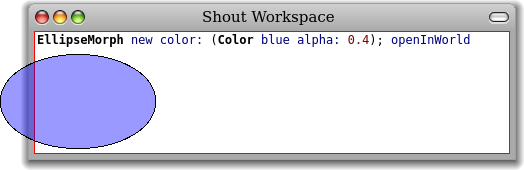
\includegraphics[scale=0.7]{TranslucentEllipse}}}
	{\centerline {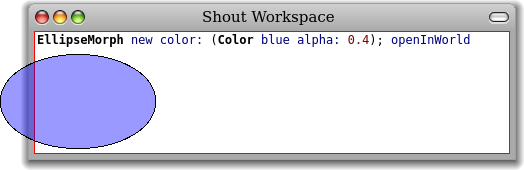
\includegraphics[width=8cm]{TranslucentEllipse}}}
\caption{Une ellipse translucide.\figlabel{translucentEllipse}}
\end{figure}
\end{center}

%%Par la \ruleref{inheritance}, 
D'après la \ruleref{inheritance},
toute classe possède une super-classe.
La super-classe de \clsind{TranslucentColor} est \clsind{Color} et la super-classe de \ct{Color} est \clsind{Object}:
\begin{code}{@TEST}
TranslucentColor superclass --> Color
Color superclass                   --> Object
\end{code}

Comme tout se produit par \subind{message}{envoi} de messages
(\ruleref{message}), nous pouvons en déduire que \mthind{Color
  class}{blue} est un message à destination de \ct{Color};
\mthind{Object}{class} et \mthind{Color}{alpha:} sont des messages à
destination de la couleur bleue; \mthind{Morph}{openInWorld} est un
message à destination d'une ellipse morph et
\mthind{Behavior}{superclass} est un message à destination de
\ct{TranslucentColor} et \ct{Color}. % REVOIR PBE message send ->
                                % sending messages
Dans chaque cas, le receveur est un objet puisque \mantra bien que certains de ces objets soient aussi des classes.

La recherche de méthodes suit la chaîne d'héritage (\ruleref{lookup}), donc quand nous envoyons le message \ct{class} au résultat de 
\ct{Color blue alpha: 0.4}, le message est traité quand la méthode correspondante est trouvée dans la classe \ct{Object}, comme illustré par \figref{classmessage}.

\begin{center}
\begin{figure}[!ht]
\ifluluelse
	{\centerline{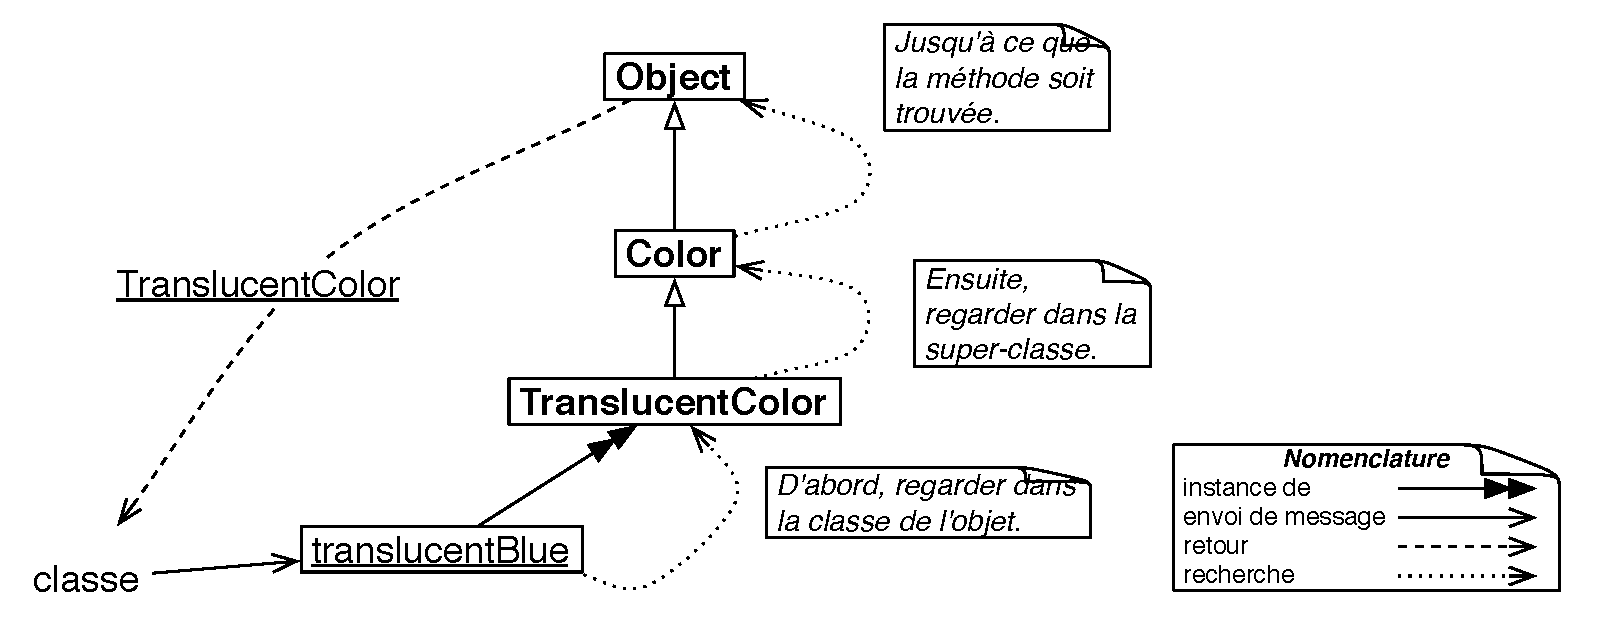
\includegraphics[width=\textwidth]{TranslucentClassMessage}}}
	{\centerline{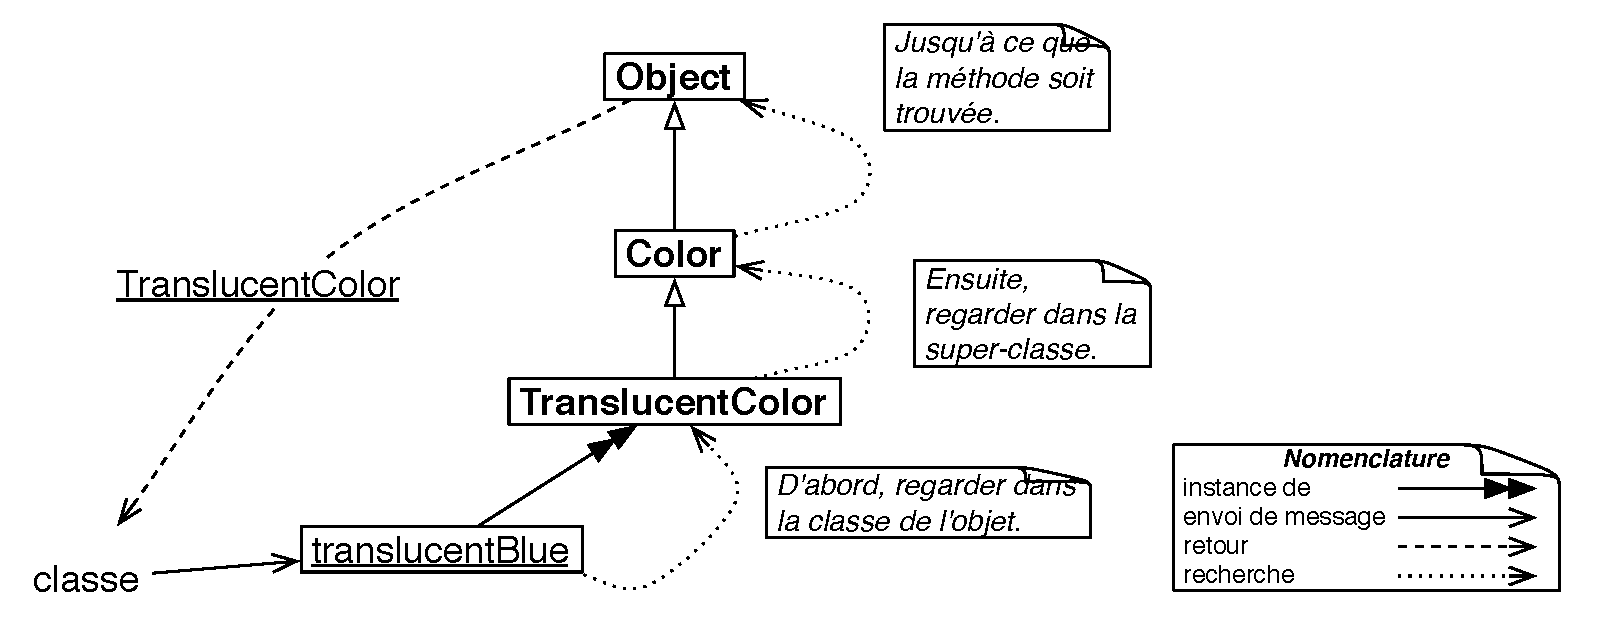
\includegraphics[width=0.8\textwidth]{TranslucentClassMessage}}}
\caption{Envoyer un message à une couleur translucide.\figlabel{classmessage}}
\end{figure}
\end{center}

Cette figure résume l'essence de la relation \emphind{est un}{}(e).
Notre objet bleu translucide \emphind{est un}{}e instance de
\ct{TranslucentColor}, mais nous pouvons aussi dire qu'il
\emph{est un}{}e  \ct{Color} et qu'il \emph{est un} \ct{Object}, puisqu'il répond aux messages définis dans toutes ces classes.
En fait, il y a un message, \mthind{Object}{isKindOf:}, qui peut être envoyé à n'importe quel objet pour déterminer s'il est en relation ``\emph{est un}'' avec une classe donnée:

\needlines{4}
\begin{code}{@TEST | translucentBlue |}
translucentBlue := Color blue alpha: 0.4.
translucentBlue isKindOf: TranslucentColor --> true
translucentBlue isKindOf: Color                    --> true
translucentBlue isKindOf: Object                  --> true
\end{code}

%=================================================================
\section{Toute classe est une instance d'une méta-classe}

% \ruleref{metaclass}

Comme nous l'avons mentionné dans \secref{metaclassIntro}, les classes dont les instances sont aussi des classes sont appelées des \ind{méta-classe}{}s.

\paragraph{Les méta-classes sont implicites.}
Les méta-classes sont automatiquement créées quand une classe est définie.
On dit qu'elles sont \emph{implicites} car en tant que programmeur, vous n'avez jamais à vous en soucier.
Une méta-classe \subind{méta-classe}{implicite} est créée pour chaque classe que vous créez donc chaque méta-classe n'a qu'une seule instance.

Alors que les classes ordinaires sont nommées par des variables globales, les méta-classes sont anonymes.
Cependant, nous pouvons toujours les référencer à travers la classe qui est leur instance.
Par exemple, la classe de \clsind{Color} est \clsind{Color class} et la classe de \ct{Object} est \clsind{Object class}:
\begin{code}{@TEST}
Color class   --> Color class
Object class --> Object class
\end{code}

\noindent
\Figref{translucentmetaclasses} montre que chaque classe est une instance de sa méta-classe (\subind{méta-classe}{anonyme}).

\begin{center}
\begin{figure}[!ht]
\ifluluelse
	{\centerline {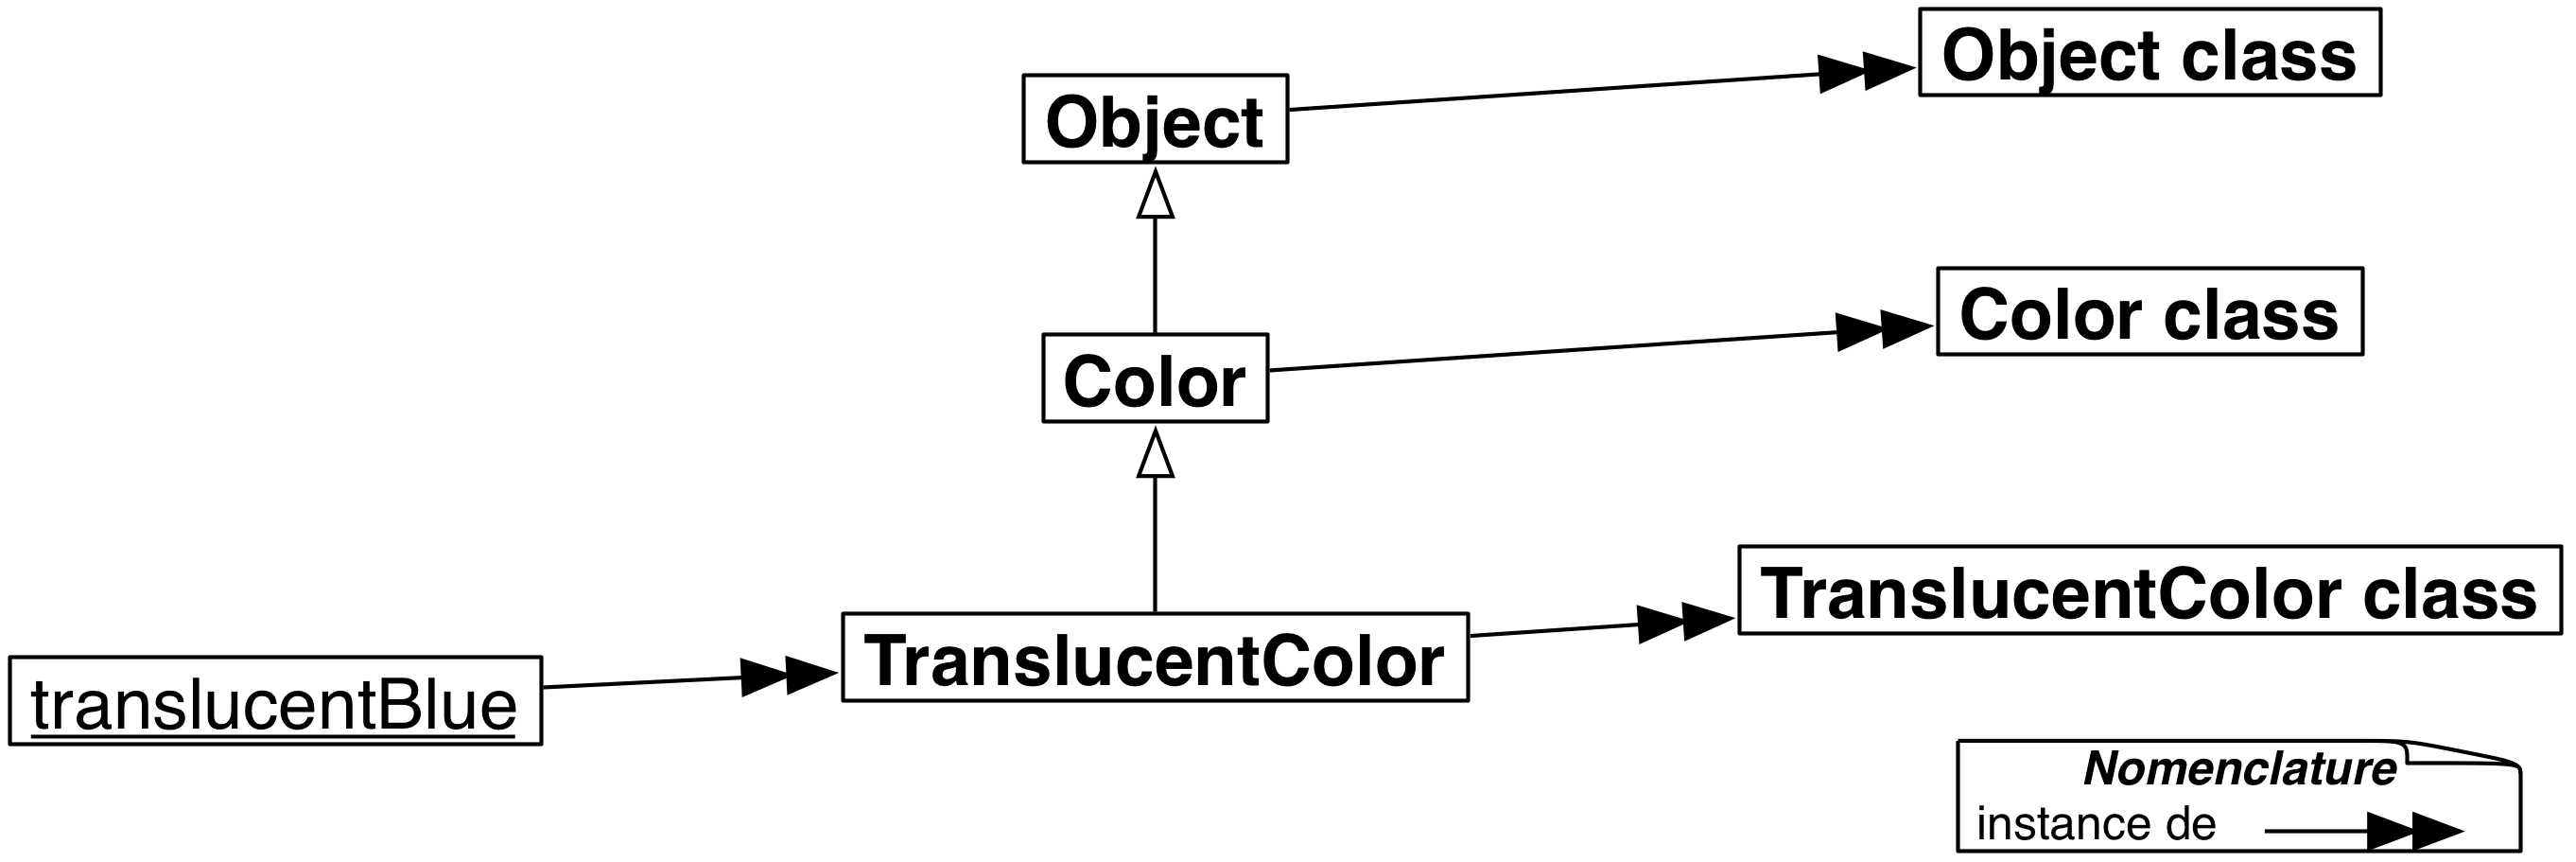
\includegraphics[width=\textwidth]{TranslucentMetaclasses}}}
	{\centerline {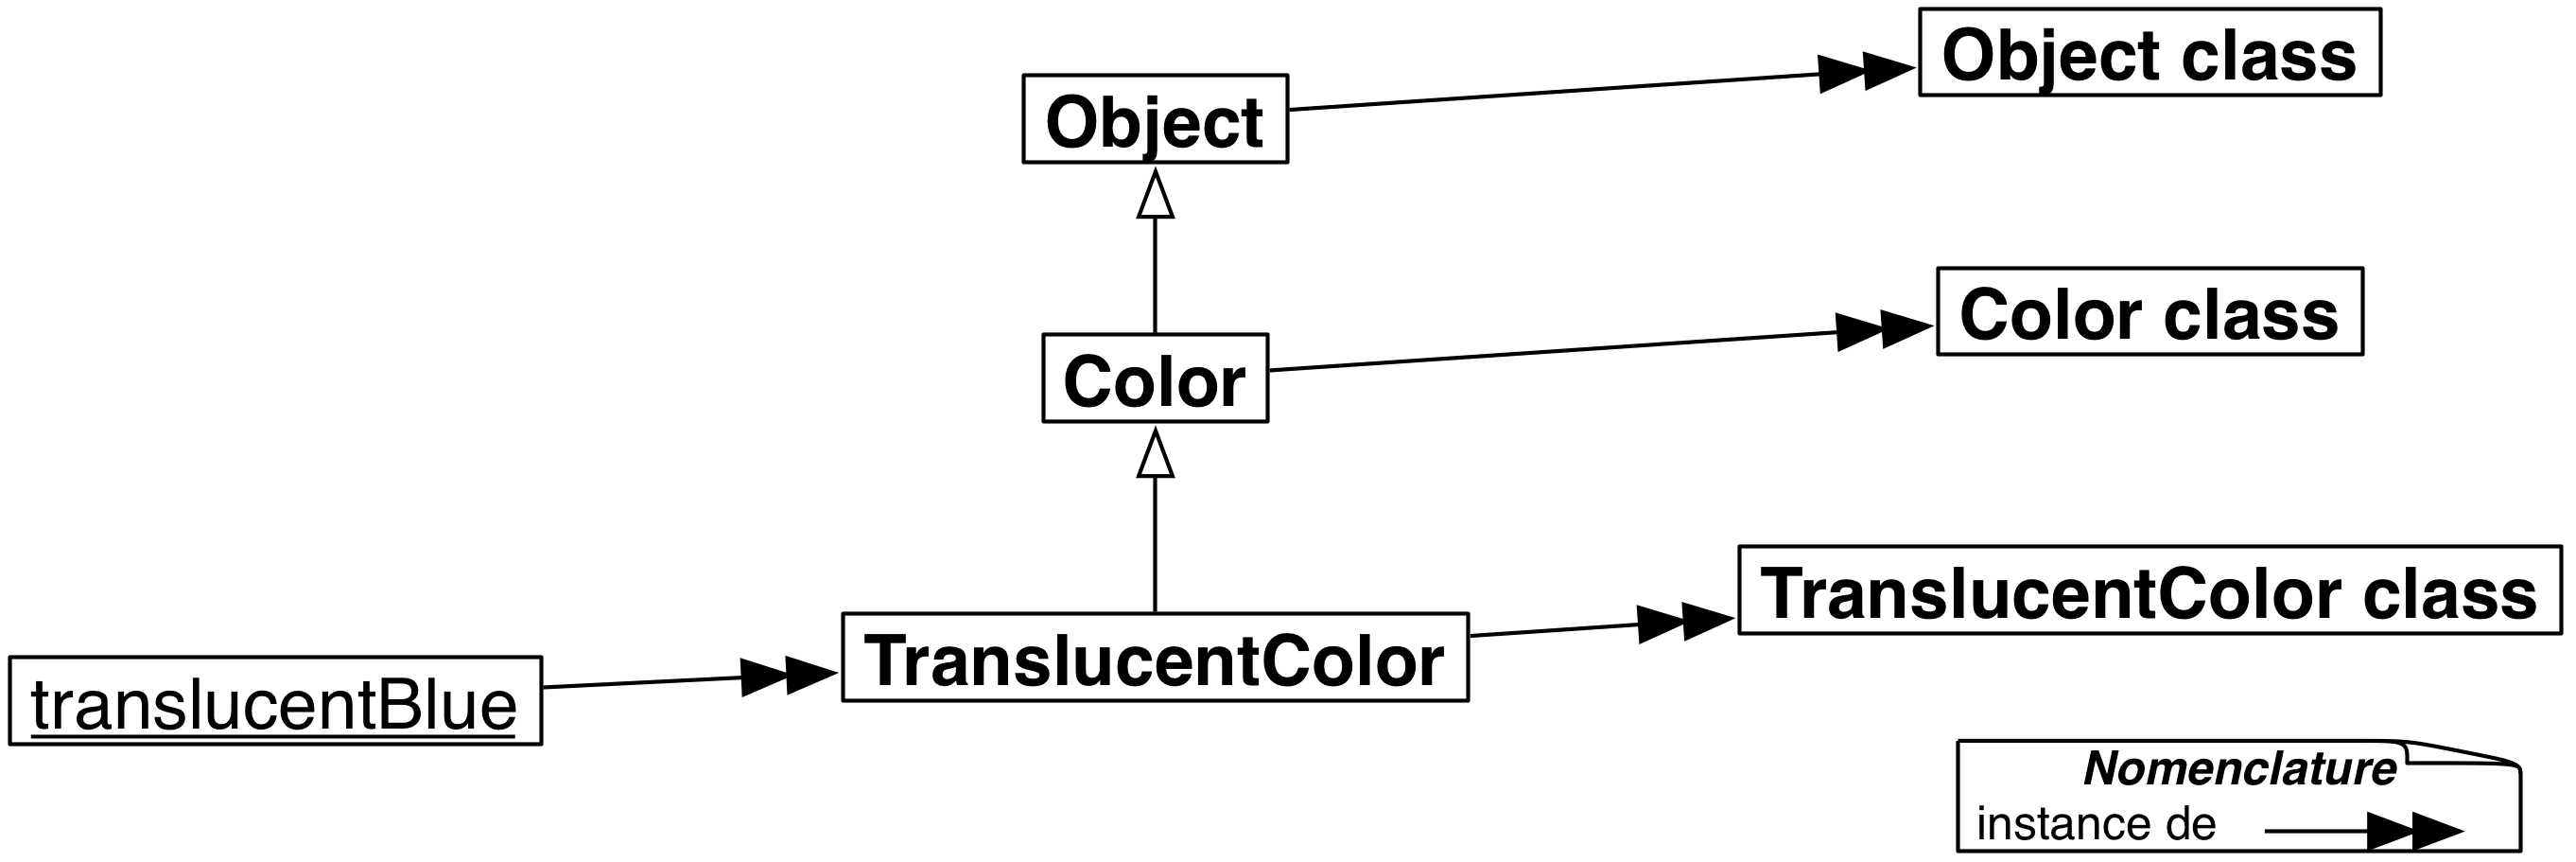
\includegraphics[width=0.8\textwidth]{TranslucentMetaclasses}}}
\caption{Les méta-classes de TranslucentColor et ses super-classes.\figlabel{translucentmetaclasses}}
\end{figure}
\end{center}


Le fait que les classes soient aussi des objets facilite leur interrogation par envoi de messages.
Voyons cela:
\begin{code}{@TEST}
Color subclasses                           --> {TranslucentColor}
TranslucentColor subclasses         --> #()
TranslucentColor allSuperclasses  --> an OrderedCollection(Color Object ProtoObject)
TranslucentColor instVarNames     --> #('alpha')
TranslucentColor allInstVarNames --> #('rgb' 'cachedDepth' 'cachedBitPattern' 'alpha')
TranslucentColor selectors             -->  an IdentitySet(#pixelValueForDepth: #pixelWord32
#convertToCurrentVersion:refStream: #isTransparent #scaledPixelValue32 #bitPatternForDepth: #storeArrayValuesOn: #setRgb:alpha: #alpha #isOpaque #pixelWordForDepth: #isTranslucentColor #hash #isTranslucent #alpha: #storeOn: #asNontranslucentColor #privateAlpha #balancedPatternForDepth:)
\end{code}
\cmindex{Class}{subclasses}
\cmindex{Behavior}{allSuperclasses}
\cmindex{Behavior}{instVarNames}
\cmindex{Behavior}{allInstVarNames}
\cmindex{Behavior}{selectors}


%=================================================================
\section{La hiérarchie des méta-classes est parallèle à celle des classes}
% \ruleref{parallelhierarchy}

La \ruleref{parallelhierarchy} dit que la super-classe d'une méta-classe ne peut pas être une classe arbitraire: elle est contrainte à être la méta-classe de la super-classe de l'unique instance de cette méta-classe.
\begin{code}{@TEST}
TranslucentColor class superclass --> Color class
TranslucentColor superclass class --> Color class
\end{code}

\noindent
C'est ce que nous voulons dire par le fait que la \subindmain{méta-classe}{hiérarchie} des méta-classes est parallèle à la hiérarchie des classes; \figref{parallelHierarchies} montre comment cela fonctionne pour la hiérarchie de \clsind{TranslucentColor}.
 
\begin{center}
\begin{figure}[!ht]
\ifluluelse
	{\centerline {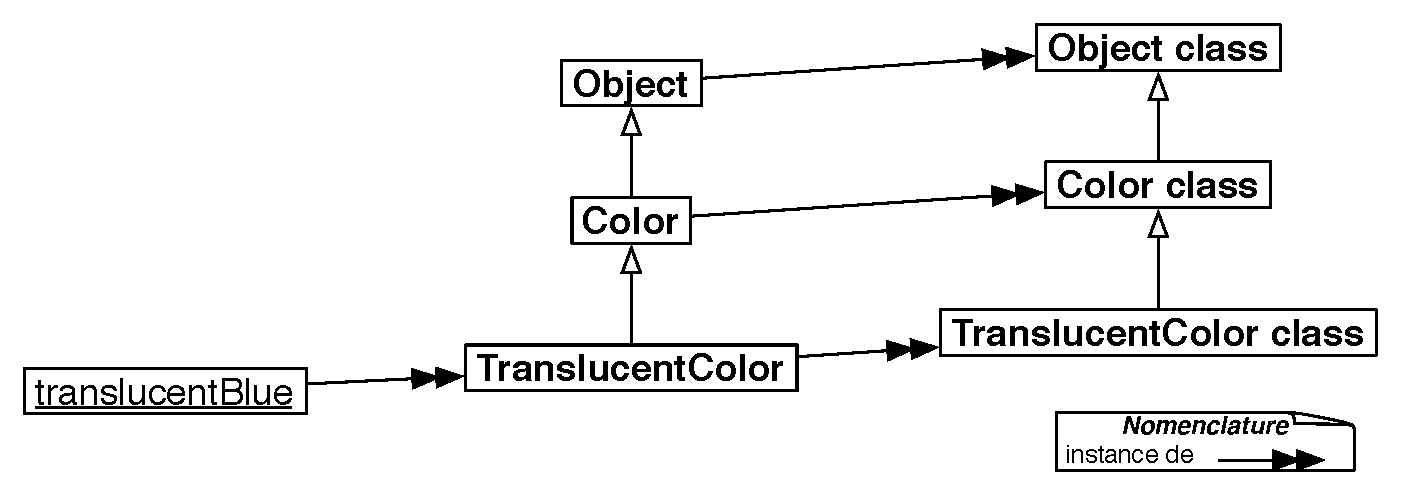
\includegraphics[width=\textwidth]{TranslucentMetaclassHierarchy}}}
	{\centerline {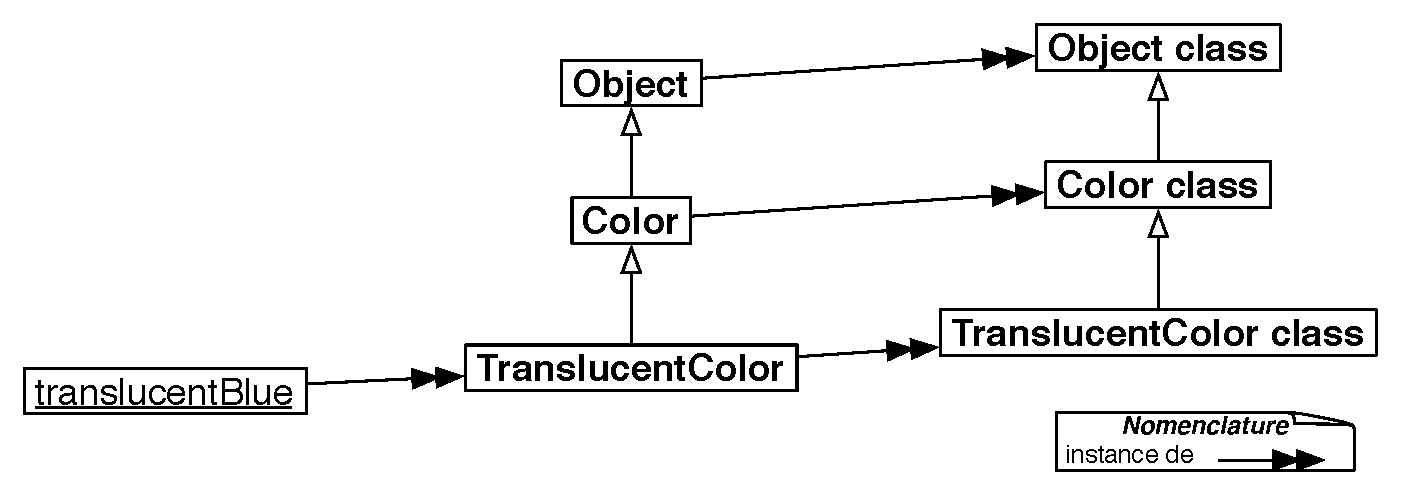
\includegraphics[width=0.8\textwidth]{TranslucentMetaclassHierarchy}}}
\caption{La hiérarchie des méta-classes est parallèle à la hiérarchie des classes.\figlabel{parallelHierarchies}}
\end{figure}
\end{center}

\begin{code}{@TEST}
TranslucentColor class                                     --> TranslucentColor class
TranslucentColor class superclass                   --> Color class
TranslucentColor class superclass superclass --> Object class
\end{code}

\paragraph{L'uniformité entre les classes et les objets.}
Il est intéressant de revenir en arrière un moment et de réaliser qu'il n'y a pas de différence entre envoyer un message à un objet et à une classe.
Dans les deux cas, la recherche de la méthode correspondante commence dans la classe du receveur et chemine le long de le chaîne d'héritage.

Ainsi, les messages envoyés à des classes doivent suivre la chaîne d'héritage des méta-classes. 
Considérons, par exemple, la méthode \mthind{Color class}{blue} qui est implémentée du \subind{Browser}{côté classe} de \ct{Color}.
Si nous envoyons le message \ct{blue} à \ct{TranslucentColor}, alors il sera traité de la même façon que les autres messages.
La recherche commence dans \ct{TranslucentColor class} et continue dans la hiérarchie des méta-classes jusqu'à trouver dans  \ct{Color class} (voir \figref{metaclasslookup}).

\begin{code}{@TEST}
TranslucentColor blue --> Color blue
\end{code}
\noindent
Notons que l'on obtient comme résultat un \ct{Color blue}  ordinaire, et non pas un translucide\,---\,il n'y a pas de magie!

\begin{center}
\begin{figure}[!ht]
\ifluluelse
	{\centerline {\includegraphics[width=\textwidth]{TranslucentColorBlue}}}
	{\centerline {\includegraphics[width=0.8\textwidth]{TranslucentColorBlue}}}
\caption{Le traitement des messages pour les classes est le même que pour les objets ordinaires.\figlabel{metaclasslookup}}
\end{figure}
\end{center}

Nous voyons donc qu'il y a une \subind{méthode}{recherche} de méthode uniforme en \st.
Les classes sont juste des objets et se comportent comme tous les autres objets.
Les classes ont le pouvoir de créer de nouvelles instances uniquement parce qu'elles répondent au message \ct{new} et que la méthode pour \ct{new} sait créer de nouvelles instances.
Normalement, les objets qui ne sont pas des classes ne comprennent pas
ce message, mais si vous avez une bonne raison pour faire cela, il n'y a rien qui vous empêche d'ajouter une méthode \ct{new} à une classe qui n'est pas une méta-classe.

Comme les classes sont des objets, nous pouvons aussi les inspecter.
\index{inspecteur}

\dothis{Inspectez \ct{Color blue} et \ct{Color}.}

%martial: la tournure reste lourde: Tue Dec 25 20:50:20 CET 2007
\noindent
Notons que vous inspectez, dans un cas, une instance de \ct{Color} et
dans l'autre cas, la classe \ct{Color} elle-même.
Cela peut prêter à confusion parce que la barre de titre de l'inspecteur contient le nom de la \emph{classe} de l'objet en cours d'inspection.
L'inspecteur sur \ct{Color} vous permet de voir 
%% ajout
entre autre la super-classe, les variables d'instances, le \subind{méthode}{dictionnaire} des méthodes 
%% etc.
de  la classe \ct{Color}, comme indiqué dans \figref{inspectingColor}.

\begin{center}
\begin{figure}[!ht]
\ifluluelse
	{\centerline{\includegraphics[width=\textwidth]{InspectingColor}}}
	{\centerline{\includegraphics[width=10cm]{InspectingColor}}}
\caption{Les classes sont aussi des objets.\figlabel{inspectingColor}}
\end{figure}
\end{center}


%=================================================================
\section{Toute m{é}ta-classe h{é}rite de \ct{Class} et de \ct{Behavior}}
% \ruleref{behavior}

Toute \ind{méta-classe} \emphind{est un}{}e classe, donc hérite de \clsind{Class}.
À son tour, \ct{Class} hérite de ses super-classes, \clsind{ClassDescription} et \clsind{Behavior}.
En \st, puisque tout \emph{est un} objet, ces classes héritent finalement toutes de \ct{Object}.
Nous pouvons voir le schéma complet dans \figref{inheritbehavior}.

\begin{center}
\begin{figure}
\ifluluelse
	{\centerline{\includegraphics[width=\textwidth]{TranslucentBehavior}}}
	{\centerline{\includegraphics[width=0.8\textwidth]{TranslucentBehavior}}}
\caption{Les méta-classes héritent de \ct{Class} et de \ct{Behavior}.\figlabel{inheritbehavior}}
\end{figure}
\end{center}


\paragraph{Où est défini \ct{new}?}
Pour comprendre l'importance du fait que les méta-classes héritent de \ct{Class} et de \ct{Behavior}, 
%% cela aide de demander 
demandons-nous
où est défini \ct{new} et comment cette définition est trouvée.
Quand le message \ct{new} est envoyé à une classe, il est recherché dans sa chaîne de méta-classes et finalement dans ses super-classes \ct{Class}, \ct{ClassDescription} et \ct{Behavior} comme montré dans \figref{sendingnew}.

La question ``\emph{Où est défini \ct{new}?}'' est cruciale.
La méthode \mthind{Behavior}{new} est définie en premier dans la classe \ct{Behavior} et peut être redéfinie dans ses sous-classes, ce qui inclut toutes les méta-classes des classes que nous avons définies, si cela est nécessaire.
Maintenant, quand un message \ct{new} est envoyé à une classe, il est recherché, comme d'habitude, dans la méta-classe de cette classe, en continuant le long de la chaîne de super-classes jusqu'à la classe \ct{Behavior} si aucune redéfinition n'a été rencontrée sur le chemin.

Notons que le résultat de l'envoi de message \ct{TranslucentColor new} est une instance de  \clsind{TranslucentColor}  et \emph{non} de \ct{Behavior}, même si la méthode est trouvée dans la classe \ct{Behavior}!  \ct{new} retourne toujours une instance de \self, la classe qui a reçu le message, même si cela est implémenté dans une autre classe.

\begin{code}{@TEST}
TranslucentColor new class --> TranslucentColor    "et non pas Behavior!"
\end{code}

\begin{center}
\begin{figure}
\ifluluelse
	{\centerline{\includegraphics[width=\textwidth]{TranslucentSendingNew}}}
	{\centerline{\includegraphics[width=0.8\textwidth]{TranslucentSendingNew}}}
\caption{\ct{new} est un message ordinaire recherché dans la chaîne des méta-classes.\figlabel{sendingnew}}
\end{figure}
\end{center}

Une erreur courante est de rechercher \ct{new} dans la super-classe de la classe du receveur.
La même chose se produit pour \ct{new:}, le message standard pour créer un objet d'une taille donnée.
Par exemple, \ct{Array new: 4} crée un tableau de 4 éléments.
Vous ne trouverez pas la définition de cette méthode dans \ct{Array} ni 
%% ajout
dans aucune de ses super-classes. À la place, vous devriez regarder dans \ct{Array class} et ses super-classes puisque c'est là que la recherche commence.

\on{The text below needs more details and convincing examples ...}

\paragraph{Les responsabilités de \ct{Behavior}, \ct{ClassDescription} et \ct{Class}.}
\clsind{Behavior} fournit l'état minimum et nécessaire à des objets possédant des instances: cela inclut un lien super-classe, un dictionnaire de méthodes et une description des instances (\ie représentation et nombre).
\on{not sure I understand the last point}% LF same for me...
\ct{Behavior} hérite de \ct{Object}, donc elle, ainsi que toutes ses sous-classes peuvent se comporter comme des objets. 

\ct{Behavior} est aussi l'interface basique pour le compilateur.
Elle fournit des méthodes pour créer un dictionnaire de méthodes, compiler des méthodes, créer des instances (\ie \mthind{Behavior}{new}, \mthind{Behavior}{basicNew}, \mthind{Behavior}{new:}, et \mthind{Behavior}{basicNew:}),
manipuler la hiérarchie de classes (\ie
\mthindex{Behavior}{superclass:} \lct{superclass:}, % CHANGE
 \mthind{Behavior}{addSubclass:}), 
accéder aux méthodes (\ie \mthind{Behavior}{selectors}, \lmthind{Behavior}{allSelectors}, \mthind{Behavior}{compiledMethodAt:}),
accéder aux instances et aux variables (\ie \mthind{Behavior}{allInstances}, \mthind{Behavior}{instVarNames}\ldots),
accéder à la hiérarchie de classes (\ie \mthind{Behavior}{superclass}, \mthind{Behavior}{subclasses})
et interroger  (\ie \mthind{Behavior}{hasMethods}, \mthind{Behavior}{includesSelector}, \mthind{Behavior}{canUnderstand:}, \mthind{Behavior}{inheritsFrom:}, \mthind{Behavior}{isVariable}).

\clsind{ClassDescription} est une classe abstraite qui fournit des facilités utilisées par ses deux sous-classes directes,  \clsind{Class} et \clsind{Metaclass}.
\clsind{ClassDescription} ajoute des facilités fournies à la base par \ct{Behavior}:
des variables d'instances nommées,
la catégorisation des méthodes dans des protocoles,
la notion de nom (abstrait),
la maintenance de \changesets, la journalisation des changements
et la plupart des mécanismes requis pour l'exportation de \changesets.


\clsind{Class} représente le comportement commun de toutes les classes.
Elle fournit un nom de classe, des méthodes de compilation, des méthodes de stockage et des variables d'instance.
Elle fournit aussi  une représentation concrète pour les noms des variables de classe et des variables de pool (\mthind{Class}{addClassVarName:}, \mthind{Class}{addSharedPool:}, \mthind{Class}{initialize}).
\ct{Class} sait comment créer des instances donc toutes les méta-classes doivent finalement hériter de \ct{Class}.


%=================================================================
\section{Toute méta-classe est une instance de \ct{Metaclass}}
% \ruleref{metaclassclass}

Les méta-classes sont aussi des objets; elles sont des instances de la classe \clsind{Metaclass} comme montré dans \figref{metaclassclass}.
Les instances de la classe \ct{Metaclass} sont les méta-classes anonymes; chacune ayant exactement une unique instance qui est une classe.

\begin{center}
\begin{figure}
\ifluluelse
	{\centerline{\includegraphics[width=\textwidth]{TranslucentMetaclassClass}}}
	{\centerline{\includegraphics[width=0.8\textwidth]{TranslucentMetaclassClass}}}
\caption{Toute méta-classe est une \ct{Metaclass}.\figlabel{metaclassclass}}
\end{figure}
\end{center}


\ct{Metaclass} représente le comportement commun des méta-classes.
Elle fournit des méthodes pour la création d'instances (\ct{sub\-class\-Of:}) permettant de créer des instances initialisées de l'unique instance \ct{Metaclass} pour l'initialisation des variables de classe, la compilation de méthodes et l'obtention d'informations à propos des classes (liens d'héritage, variables d'instance, \etc).

% It provides methods for instance creation (\ct{sub\-class\-Of:})
% creating initialized instances of the metaclass's sole instance,
% initialization of class variables,
% metaclass instance, % LF "metaclass instance," non traduit car non compris dans la phrase anglaise ...
% % (\ct{name:inEnvironment:subclassOf:})
% % Actually, this is in ClassBuilder, it seems!
% method compilation, % (different semantics can be introduced)
% and class information (inheritance links, instance variables, \etc).
% \ab{This is too cryptic for me.} % LF for me too !

%=================================================================
\section{La méta-classe de \ct{Metaclass} est une instance de \ct{Metaclass}}
% \ruleref{metaclassmetaclass}

La dernière question à laquelle il faut répondre est: quelle est la classe de \clsind{Metaclass class}?
La réponse est simple: il s'agit d'une méta-classe, donc forcément une instance de \ct{Metaclass}, exactement comme toutes les autres méta-classes dans le système (voir \figref{metaclassclassclass}).


\begin{center}
\begin{figure}
\ifluluelse
	{\centerline{\includegraphics[width=\textwidth]{TranslucentMetaclassClassClass}}}
	{\centerline{\includegraphics[width=0.8\textwidth]{TranslucentMetaclassClassClass}}}
\caption{Toutes les méta-classes sont des instances de la classe \ct{Metaclass},  même la méta-classe de \ct{Metaclass}. \figlabel{metaclassclassclass}}
\end{figure}
\end{center}

La figure montre que toutes les méta-classes sont des instances de \ct{Metaclass}, ce qui inclut aussi la méta-classe de \ct{Metaclass}.
Si vous comparez les figures \ref{fig:metaclassclass} et \ref{fig:metaclassclassclass}, vous verrez comment la \subind{méta-classe}{hiérarchie} des méta-classes reflète parfaitement la hiérarchie des classes, tout le long du chemin jusqu'à \ct{Object class}.


Les exemples suivants montrent comment il est possible d'interroger la hiérarchie de classes afin de démontrer que \figref{metaclassclassclass} est correcte.
%martial: j'ai enleve les parentheses
En réalité, vous verrez que nous avons dit un pieux mensonge\,---\,\ct{Object class superclass -->} {\clsind{ProtoObject class}, et non \ct{Class}. En \pharo, il faut aller une super-classe plus haut dans la hiérarchie pour atteindre \ct{Class}.

\needlines{2}
\begin{example}{La hiérarchie des classes}{@TEST}
TranslucentColor superclass			--> Color
Color superclass			        --> Object
\end{example}

\needlines{4}
% Martial: trouver mieux que "saute". Les ! sont nécessaires pour l'espace avant le : 
\begin{example}{La hi{é}rarchie parall{è}le des méta-classes}{@TEST}
TranslucentColor class superclass          --> Color class
Color class superclass                     --> Object class
Object class superclass superclass         --> Class    "!Attention: saute ProtoObject class!"
Class superclass                           --> ClassDescription
ClassDescription superclass                --> Behavior
Behavior superclass                        --> Object
\end{example}

\begin{example}{Les instances de \ct{Metaclass}}{@TEST}
TranslucentColor class class        --> Metaclass
Color class class                   --> Metaclass
Object class class                  --> Metaclass
Behavior class class                --> Metaclass
\end{example}

\begin{example}{\ct{Metaclass class} est une \ct{Metaclass}}{@TEST}
Metaclass class class --> Metaclass
Metaclass superclass --> ClassDescription
\end{example}

%=================================================================
\section{Résumé du chapitre}

Maintenant, vous devriez mieux comprendre la façon dont les classes sont organisées et l'impact de l'uniformité du modèle objet.
Si vous vous perdez ou que vous vous embrouillez, vous devez toujours vous rappeler que l'envoi de messages est la clé: cherchez alors la méthode dans la classe du receveur.
Cela fonctionne pour \emph{tous} les receveurs.
Si une méthode n'est pas trouvée dans la classe du receveur, elle est recherchée dans ses super-classes.


\begin{enumerate}

\item Toute classe est une instance d'une méta-classe.
Les méta-classes sont implicites.
Une méta-classe est créée automatiquement à chaque fois que vous créez une classe; cette dernière étant sa seule instance.


\item La \subind{méta-classe}{hiérarchie} des méta-classes est parallèle à celle des classes.
La recherche de méthodes pour les classes est analogue à la recherche de méthodes pour les objets ordinaires et suit la chaîne des super-classes entre méta-classes.


\item Toute méta-classe hérite de \clsind{Class} et de \clsind{Behavior}.
Toute classe \emph{est un}{}e \ct{Class}.
Puisque les méta-classes sont aussi des classes, elles doivent hériter de  \ct{Class}.
	\ct{Behavior} fournit un comportement commun à toutes les entités ayant des instances.

\item Toute méta-classe est une instance de \clsind{Metaclass}.
	\ct{ClassDescription} fournit tout ce qui est commun à \ct{Class} et à \ct{Metaclass}.
	

\item La méta-classe de \ct{Metaclass} est une instance de \ct{Metaclass}.
	La relation \emph{instance-de} forme une boucle fermée, donc \ct{Metaclass class class --> Metaclass}.
\end{enumerate}

%=================================================================
\ifx\wholebook\relax\else\end{document}\fi
%=================================================================

%-----------------------------------------------------------------
